\chapter{Results and Conclusions}
\label{chap:results}

This chapter outlines the results of the experiments performed using the methods outlined in the preceding chapter. This section is split into two sections. The first section examines the effect of mapping the higher dimensional feature space to a lower dimensional representation using the methods described in section \ref{sec:experiment-features}. The second section presents an investigation into the quality of each of the mappings produced in the first section.

\section{Comparison of Real and Synthetic Datasets}

For each of the experiments in this section the full set of 360 real images of both left, right and mediolateral oblique and craniocaudal views. The set of phantom mammograms used in this project consisted of 60 images but each image corresponds to only a single ``case". Because of this limitation a single breast phantom from each case was selected at random to be included in the data used for the experiments, brining the total number of images used in all experiments to 366.

Features extracted from both sets of images are compared using a two sample Kolmogorov-Smirnov (KS) test and are reported in the relevant section. Three dimensionality reduction algorithms were tested with each of the different feature sets and visualisation of the feature space in both 2 and 3 dimensions are shown for each.

\subsection{Blob features} 
The results for the two sample KS test between the real and synthetic datasets for blob features detected over 10 scales are shown in table \ref{table:blob_features_ks}. An explanation of what each type of feature means can be found in section \ref{subsubsec:implementation-blob-features}. 2D projections of the blob feature space as produced by t-SNE, Isomap and locally linear embedding are shown in figures \ref{fig:blob_SNE_mapping}, \ref{fig:blob_iso_mapping}, and \ref{fig:blob_LLE_mapping} respectively. 

In each of the figures the real mammograms are shown as coloured dots and the breast phantoms are shown as coloured triangles. The labels corresponding to the colours used in each visualisations are the the image's BIRADS class (in the case of real mammograms) or the volumetric breast density (VBD) (in the case of breast phantoms).

Generally speaking the phantom mammograms are shown to be very different from the real mammograms features used. The distribution of blobs detected in the phantom mammograms are generally larger and contain much less small scale structure when compare to real mammograms. This is reflected in the projections for the feature space. In the t-SNE projections it can be seen that all of the phantoms blobs, regardless of VBD, are grouped towards clusters of containing a relatively high proportion of BIRADS risk class 2 \& 3 images. The projections produced by Isomap and LLE move the phantom mammograms much more clearly separate the phantoms from the real mammographic data. In the 3D LLE projection a clear banding can be seen with outliers being shown far out in the right of the image. This more clearly shows that the major underlying separating factor at work in the data is relative number of smaller and larger blobs detected. 

\begin{table}[H]
\label{table:blob_features_ks}
\centering
\primitiveinput{tables/blob_features_ks}
\caption{Comparison of the Kolmogorov-Smirnov test results for each feature generated from the radii of blobs detected in an image between real and phantom mammograms.}
\end{table}

\clearpage

\begin{figure}[H]
	\centering
	\subfigure{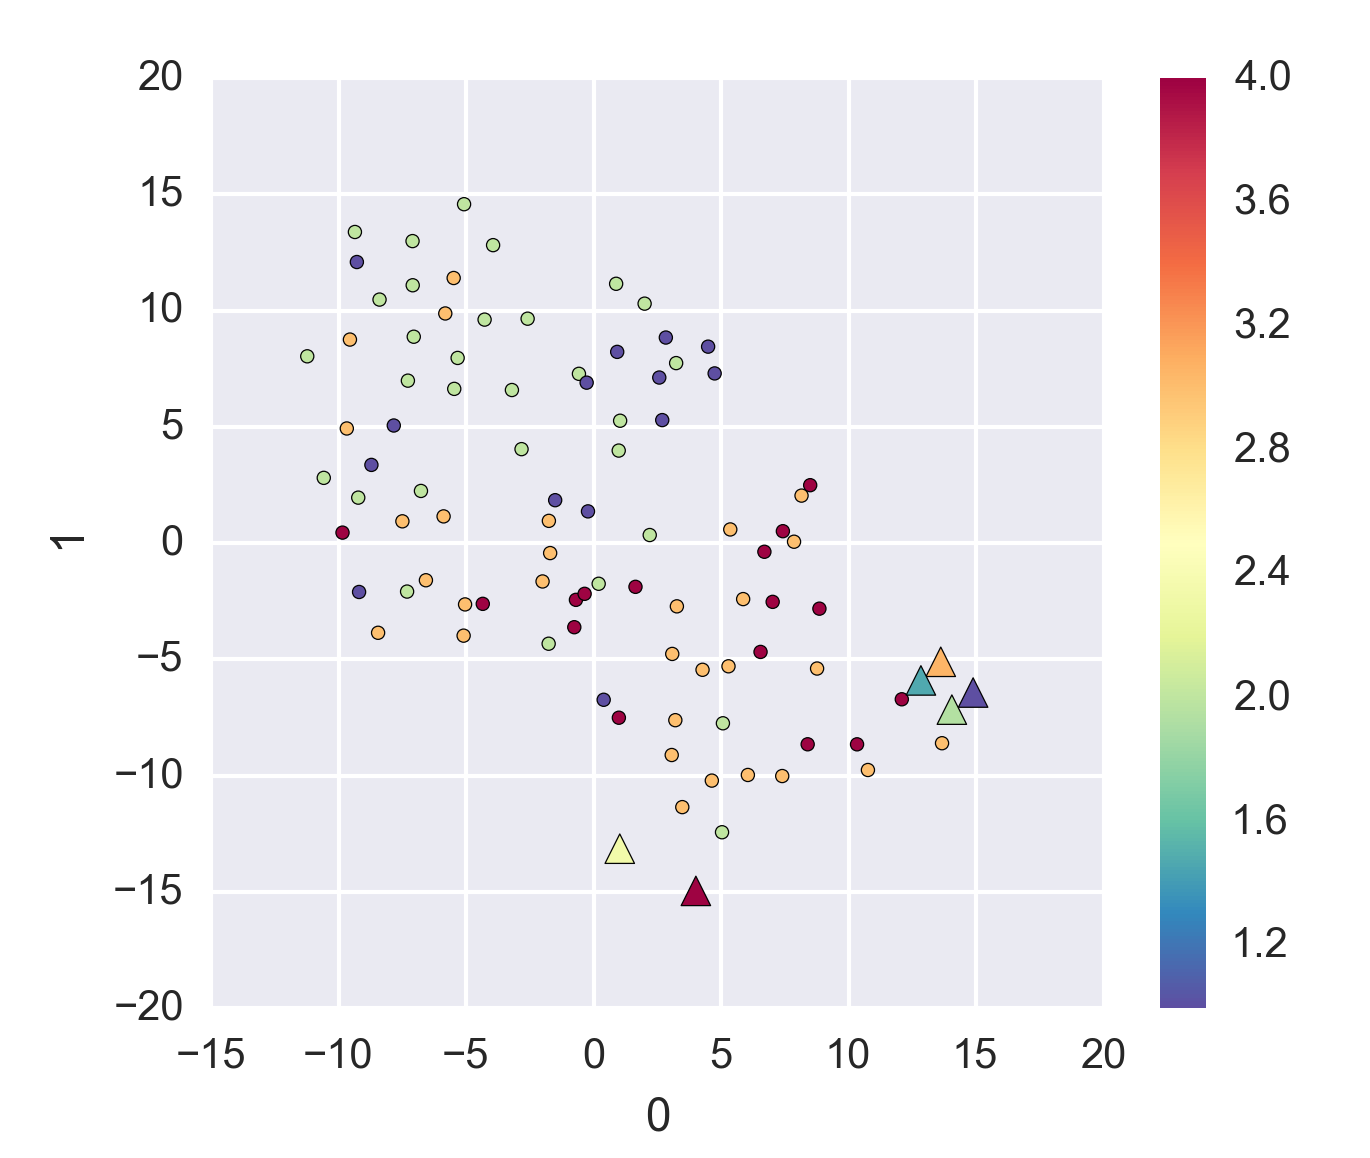
\includegraphics[width=0.49\textwidth]{figures/mappings/blob_SNE_mapping_2d.png}}
	\subfigure{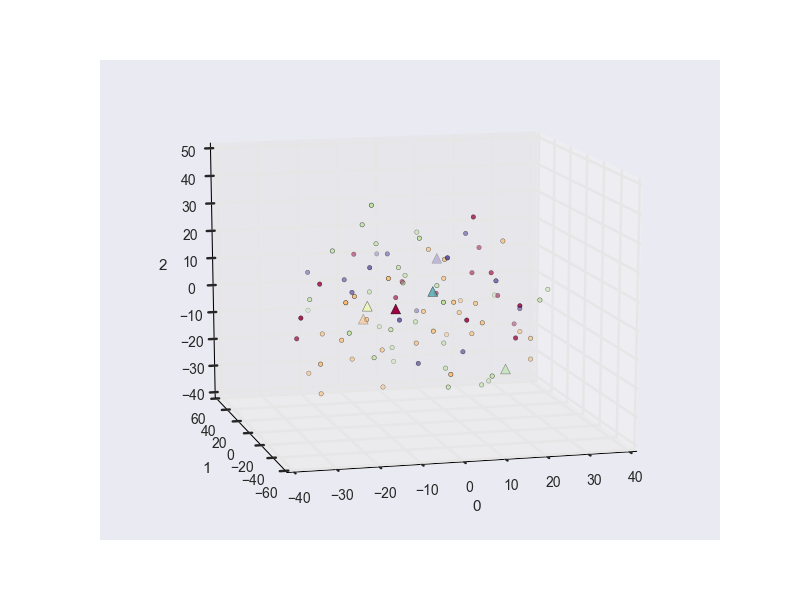
\includegraphics[width=0.49\textwidth]{figures/mappings/blob_SNE_mapping_3d.png}}
	\caption{2D \& 3D projections of the blob feature space produced by the t-SNE algorithm with a learning rate of 300 and perplexity of 30.}\label{fig:blob_SNE_mapping}
\end{figure}

\begin{figure}[H]
	\centering
	\subfigure{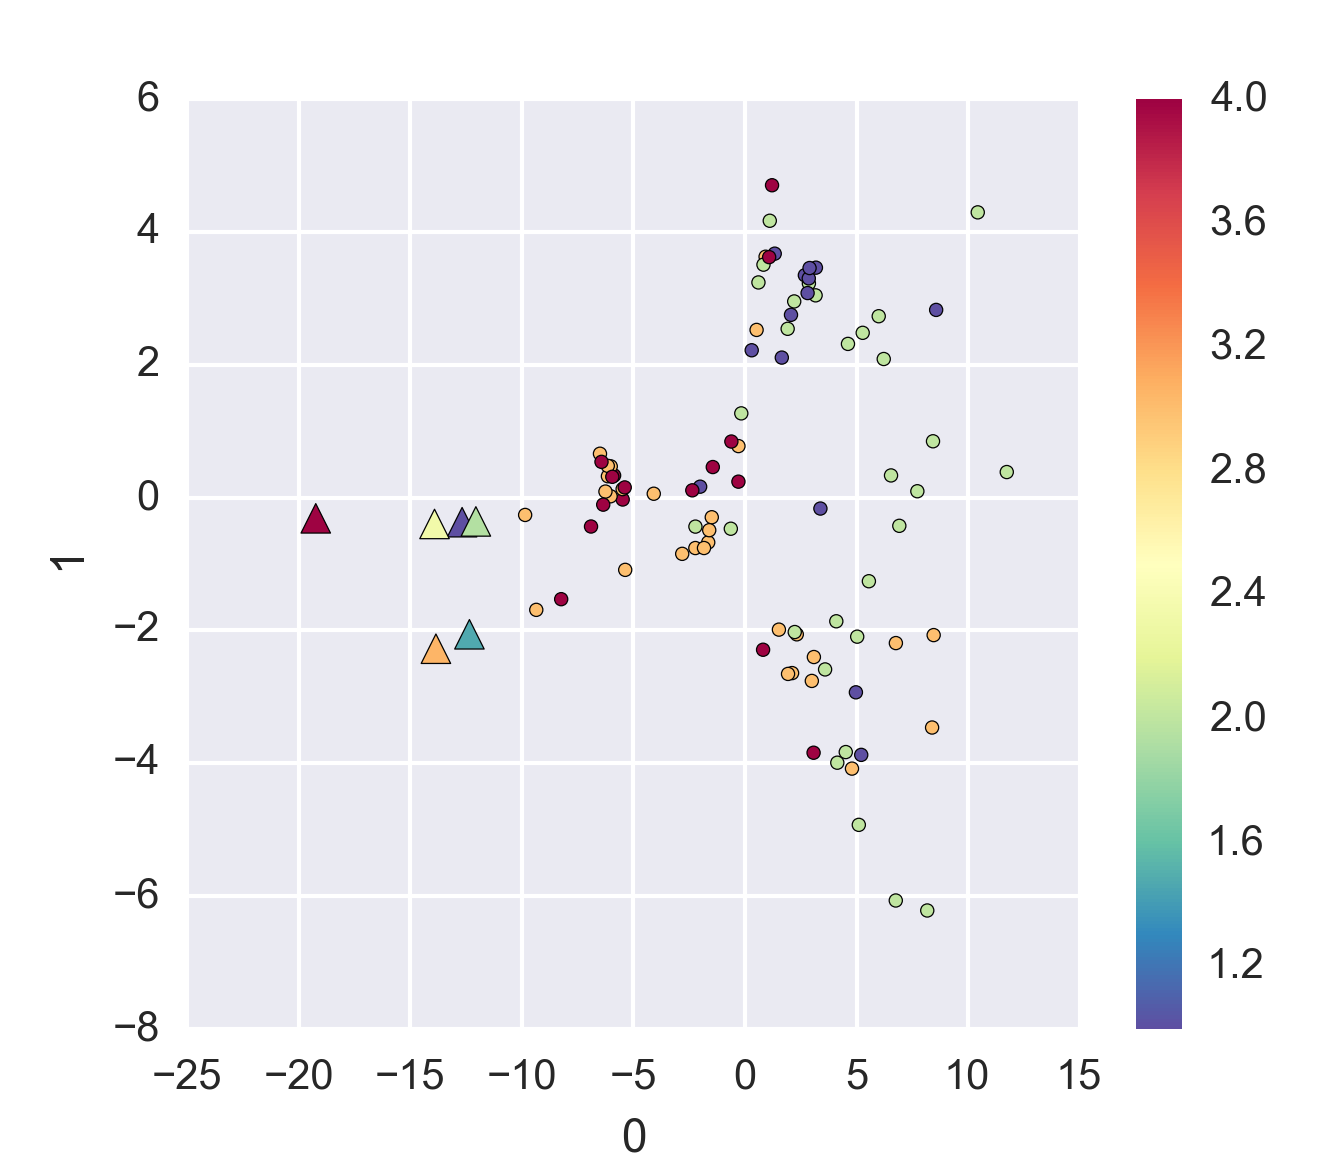
\includegraphics[width=0.49\textwidth]{figures/mappings/blob_iso_mapping_2d.png}}
	\subfigure{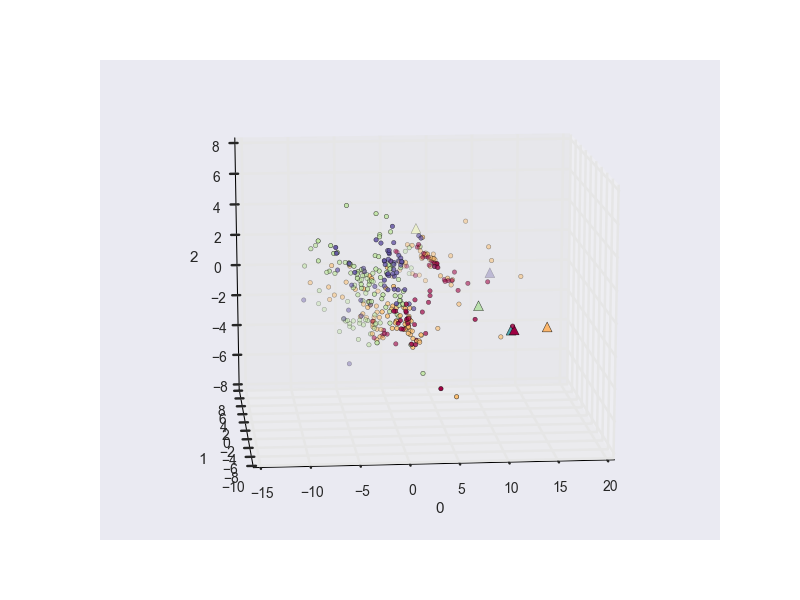
\includegraphics[width=0.49\textwidth]{figures/mappings/blob_iso_mapping_3d.png}}
	\caption{2D \& 3D projections of the blob feature space  produced by the Isomap algorithm with 50 neighbours.}\label{fig:blob_iso_mapping}
\end{figure}

\begin{figure}[H]
	\centering
	\subfigure{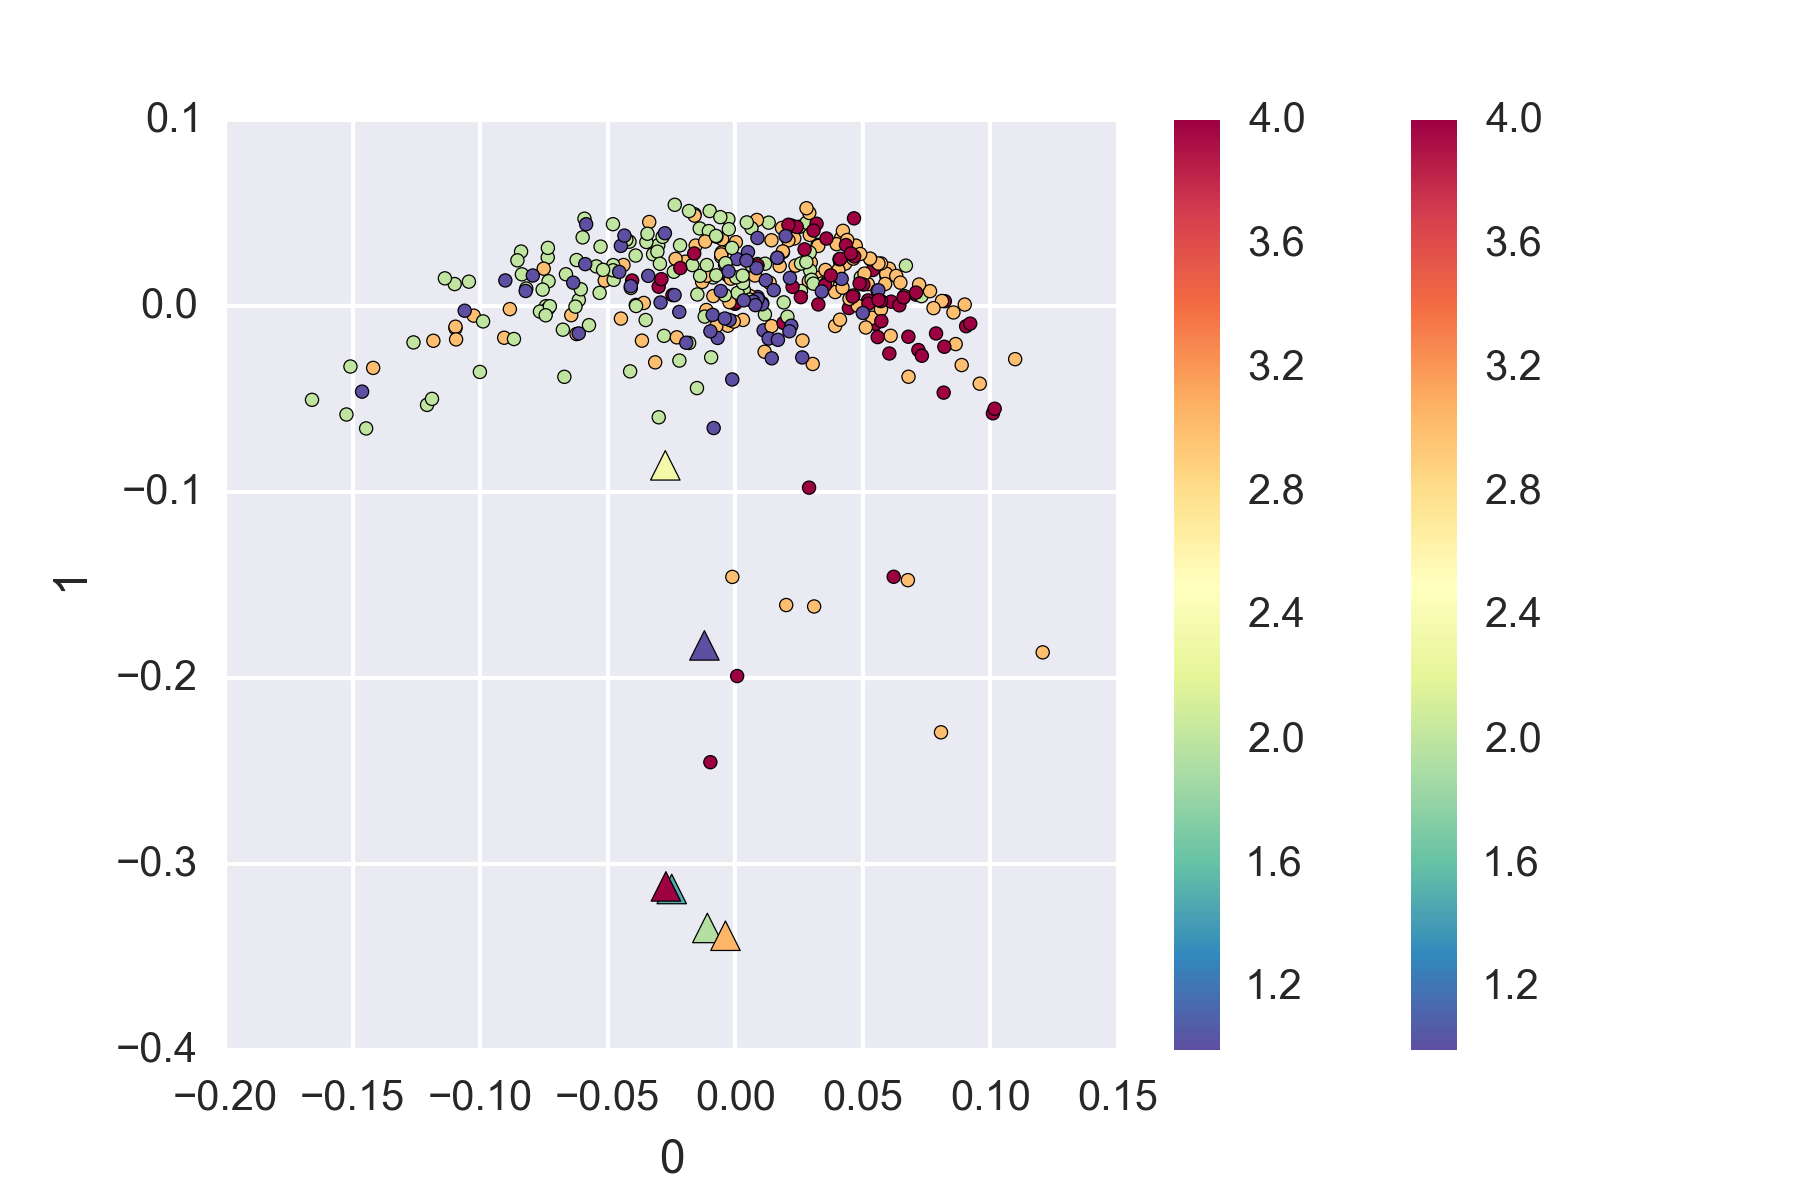
\includegraphics[width=0.49\textwidth]{figures/mappings/blob_lle_mapping_2d.png}}
	\subfigure{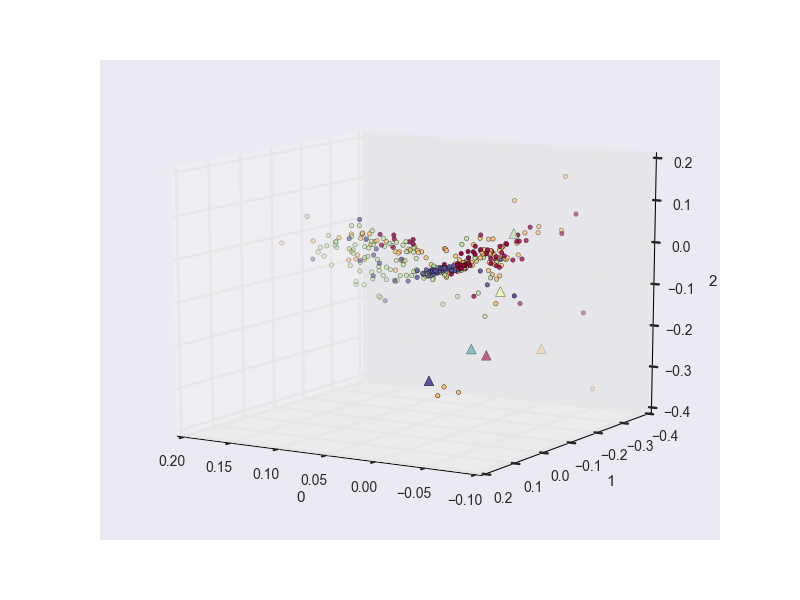
\includegraphics[width=0.49\textwidth]{figures/mappings/blob_lle_mapping_3d.png}}
	\caption{2D \& 3D projections of the blob feature space produced by the LLE algorithm with 50 neighbours.}\label{fig:blob_LLE_mapping}
\end{figure}

\clearpage

\subsection{Line features}
Results for the KS two sample test between the two feature spaces can be seen in table \ref{table:line_features_ks}. Again, as with blobs, the distributions for real and synthetic mammograms are not in particularly good agreement according to the test. 2D and 3D Projections for the line feature space for each of the three different dimensionality reduction algorithms are shown in figures \ref{fig:line_SNE_mapping}, \ref{fig:line_iso_mapping}, and \ref{fig:line_LLE_mapping} respectively.
 
\begin{table}[H]
\label{table:line_features_ks}
\centering
\primitiveinput{tables/line_features_ks}
\caption{Comparison of the Kolmogorov-Smirnov test results for each feature generated from the area of lines detected in an image between real and phantom mammograms.}
\end{table}

All of the line space projections show the same general relationship across the data. It can be seen that there is a general transition from images which contain a high mean area of linear structure on the left towards images which have a lower mean area on the right. In terms of BIRADS risk it can be seen that very low and very high risk classes are grouped towards the left, reflecting that less liner structure is detected using the orientated bins method in low risk class (because there's very little dense structure present) and high risk classes (because dense areas are mostly large, homogenous blobs not linear structure). As can be clearly seen from the visualisation the synthetic images are grouped towards the lower end reflecting the smaller size of the linear structures detected. 

The small cluster present in both the 2D and 3D projections in t-SNE and in the projections produced by LLE are caused by the min area. The cases inside the cluster contain a much larger min area compared with those present in the main cluster. This is most likely caused by a thresholding issue causing some unwanted smaller areas to be retained.


\clearpage
\begin{figure}[H]
	\centering
	\subfigure{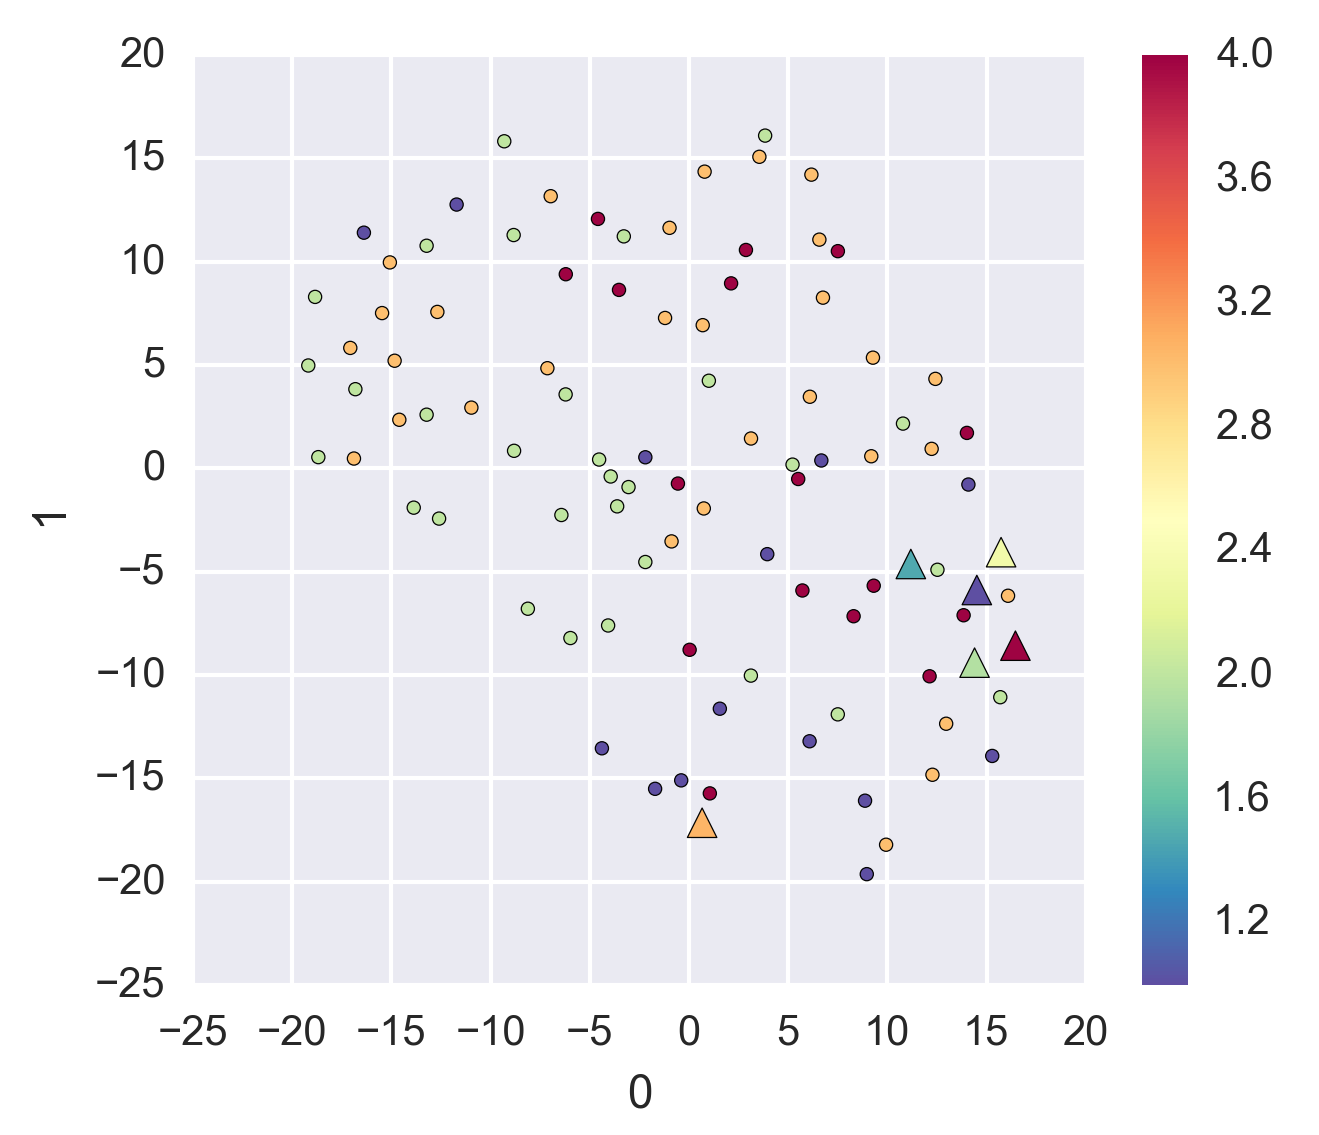
\includegraphics[width=0.49\textwidth]{figures/mappings/line_SNE_mapping_2d.png}}
	\subfigure{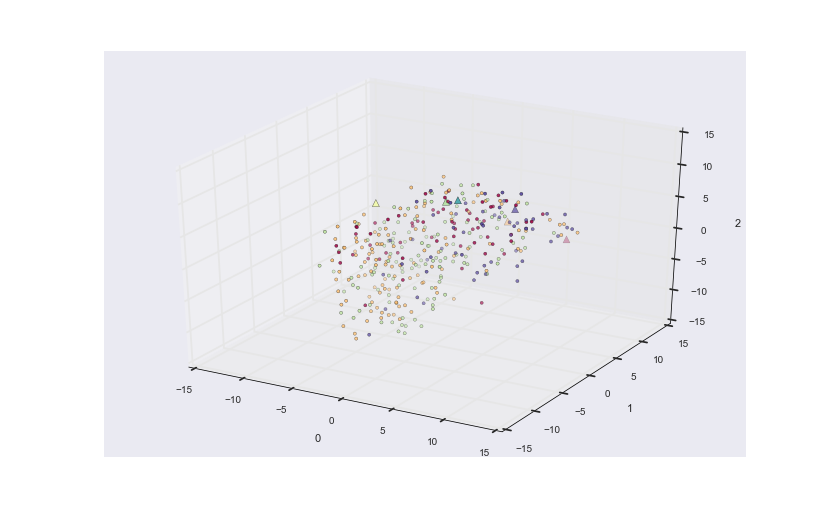
\includegraphics[width=0.49\textwidth]{figures/mappings/line_SNE_mapping_3d.png}}
	\caption{2D \& 3D projections of the line feature space produced by the t-SNE algorithm with a learning rate of 300 and perplexity of 30.}\label{fig:line_SNE_mapping}
\end{figure}

\begin{figure}[H]
	\centering
	\subfigure{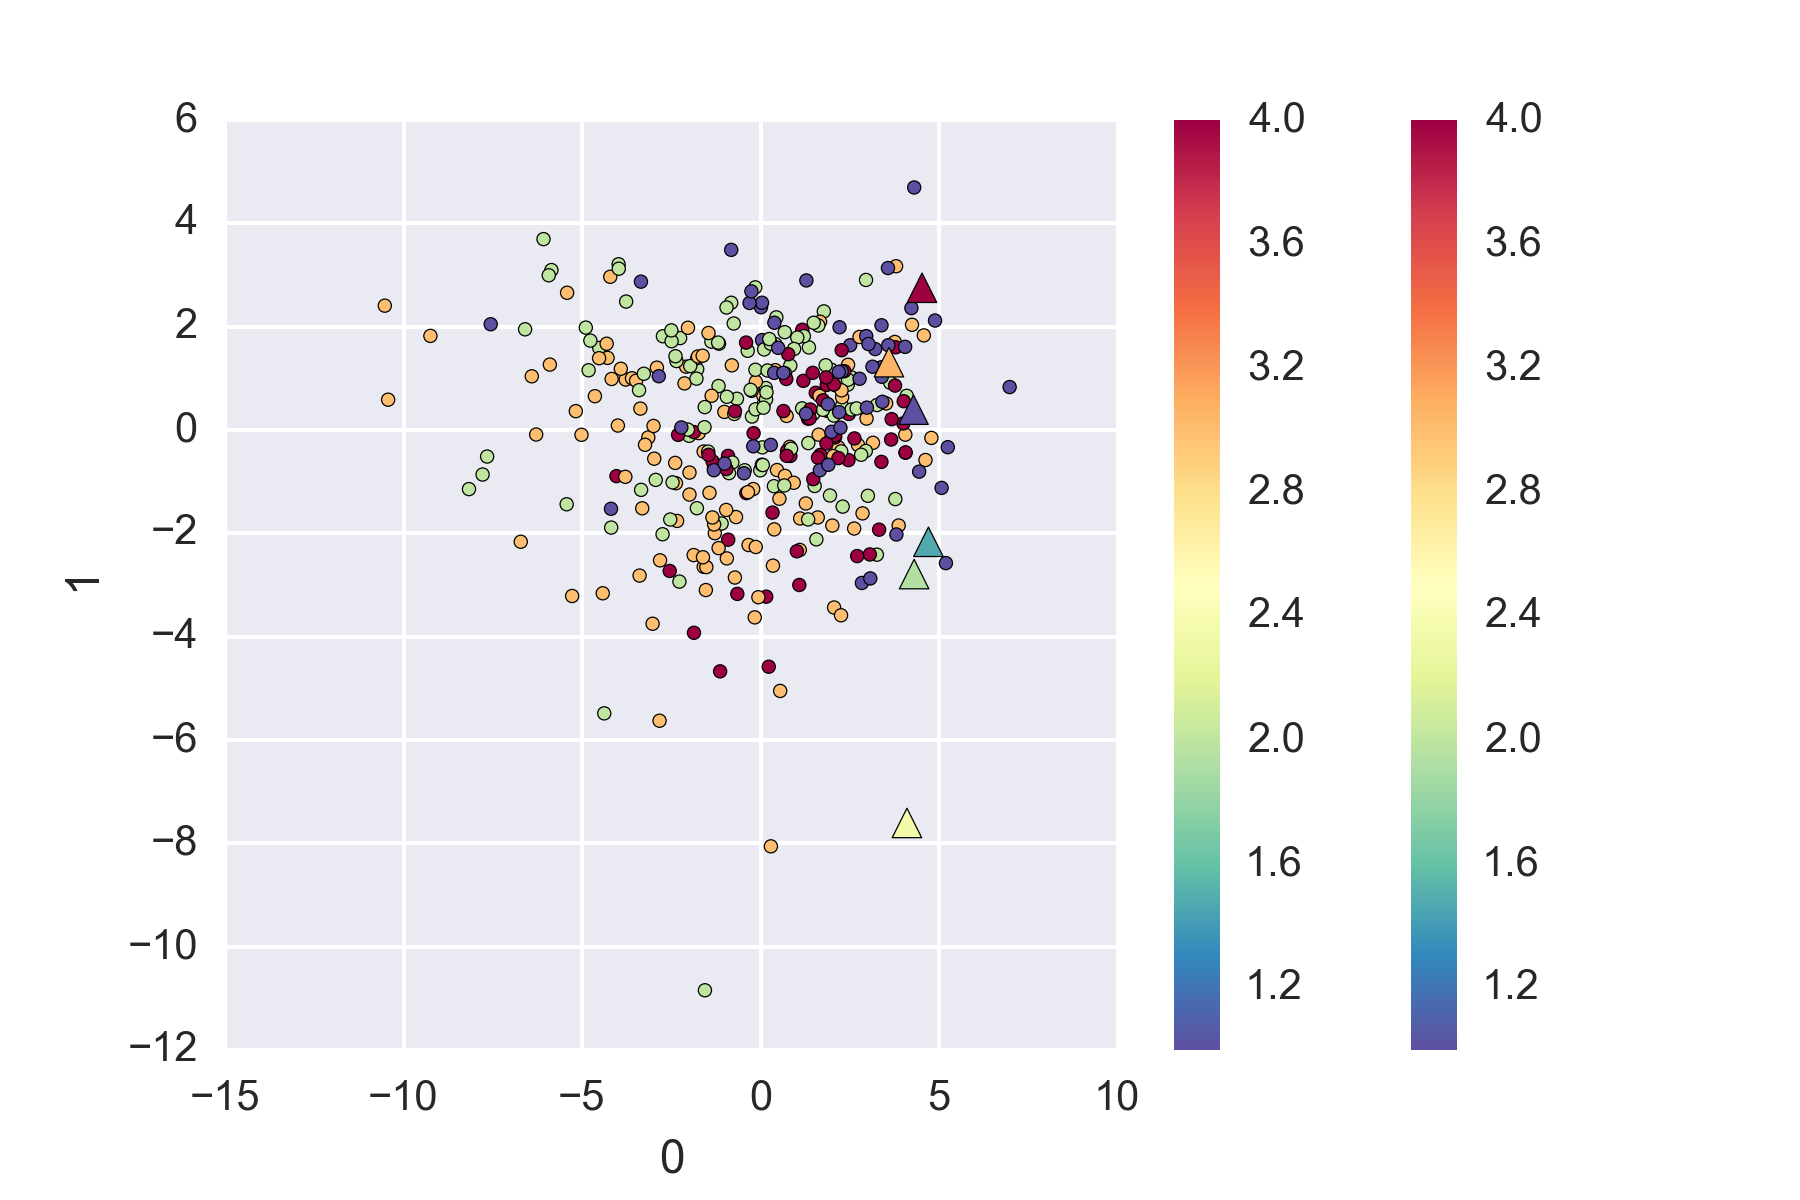
\includegraphics[width=0.49\textwidth]{figures/mappings/line_iso_mapping_2d.png}}
	\subfigure{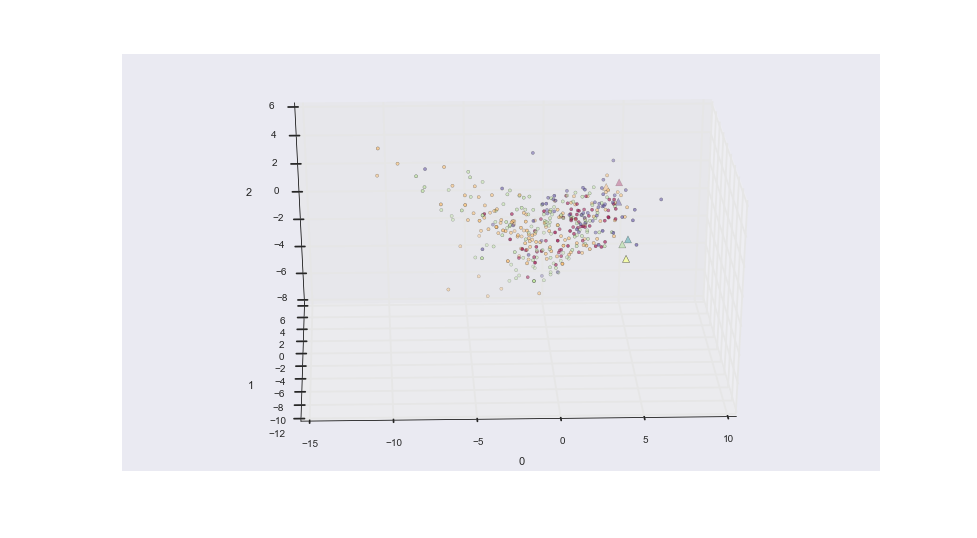
\includegraphics[width=0.49\textwidth]{figures/mappings/line_iso_mapping_3d.png}}
	\caption{2D \& 3D projections of the line feature space  produced by the Isomap algorithm with 50 neighbours.}\label{fig:line_iso_mapping}
\end{figure}

\begin{figure}[H]
	\centering
	\subfigure{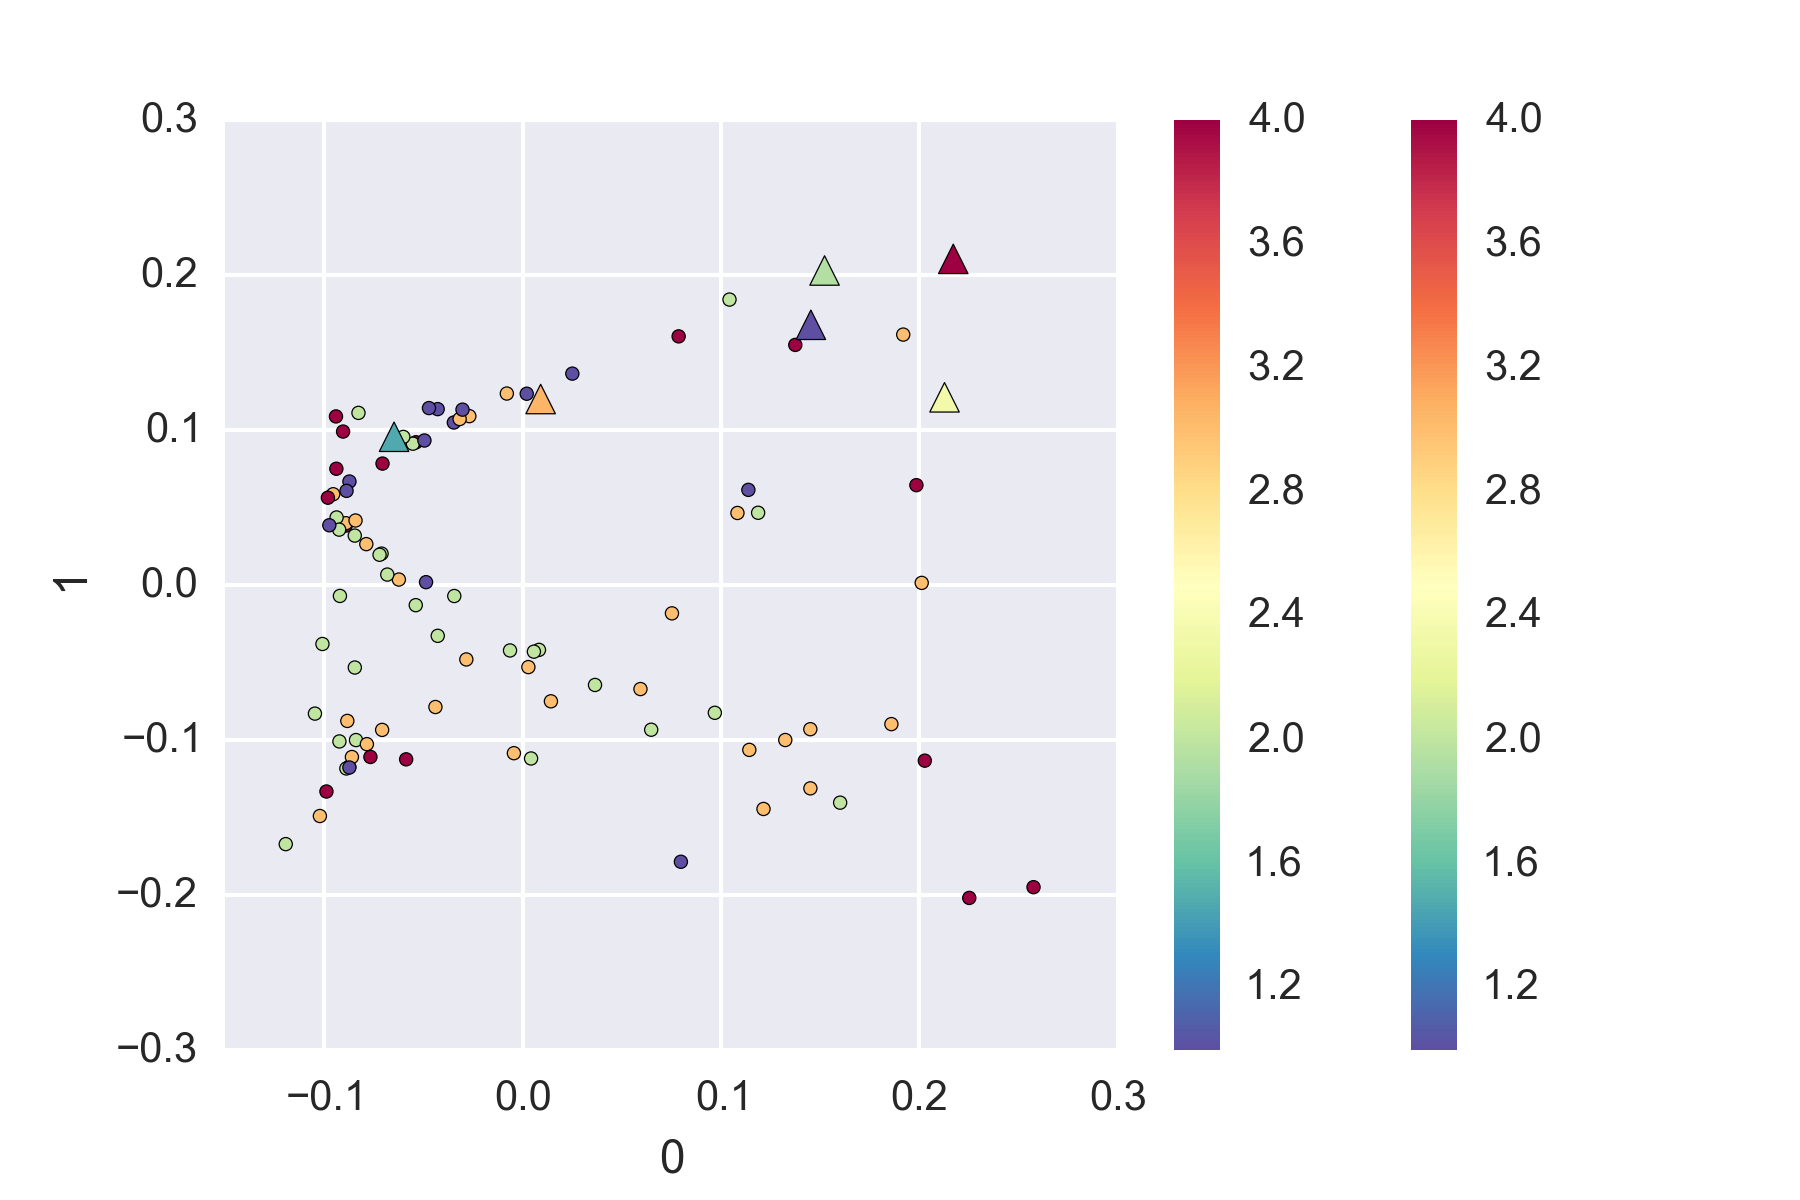
\includegraphics[width=0.49\textwidth]{figures/mappings/line_lle_mapping_2d.png}}
	\subfigure{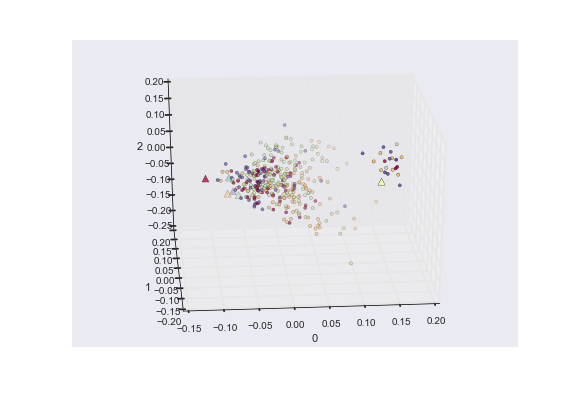
\includegraphics[width=0.49\textwidth]{figures/mappings/line_lle_mapping_3d.png}}
	\caption{2D \& 3D projections of the line feature space produced by the LLE algorithm with 50 neighbours.}\label{fig:line_LLE_mapping}
\end{figure}
\clearpage

\subsection{Intensity \& Texture Features}
\label{subsec:results-texture}
Intensity and texture features proved proved the least successful for the comparison of the real and phantom datasets. As can be seen in figure \ref{fig:mammogram-histogram} the intensity distribution of the phantom mammograms are nothing like a real mammogram. Because of this difference the results show that the they are clearly in different spaces. The results of the KS two sample test showed that the two distributions generated for both intensity and texture features are completely different. 

Due to this large difference only the results of texture features for the blob feature space are presented here. The projections for the texture features derived from the line feature space are much the same as the results shown here but are much nosier. It is suggested that the difference the results of the texture feature space derived from blobs and lines is due to the fact of that blob feature make use of scale space which allows for better risk class separation.

The results of performing dimensionality reduction on both of these feature spaces is that in all cases the synthetic mammograms are separated from the real mammograms into an isolated cluster on there own. This is because the values for both types of feature are on average much higher for the breast phantoms than the real mammograms.

It can be seen that between the real mammograms there is a trend visible in both intensity and textural features which causes some transition between high to low risk. This is particularly visible for intensity features in the 2D plot produced by t-SNE shown in figure \ref{fig:intensity_SNE_mapping} and in the 2D plot in figure \ref{fig:texture_SNE_mapping} for texture features. In the case of intensity features this transition is caused by blobs that are composed of blobs which are of higher intensity. For texture features the trend across the data is explained by a transition for blobs with low contrast and dissimilarity and high homogeneity and energy corresponding to high risk blobs transitioning through to low risk blobs where the reverse is true.

\begin{figure}
	\label{fig:mammogram-histogram}
	\centering
	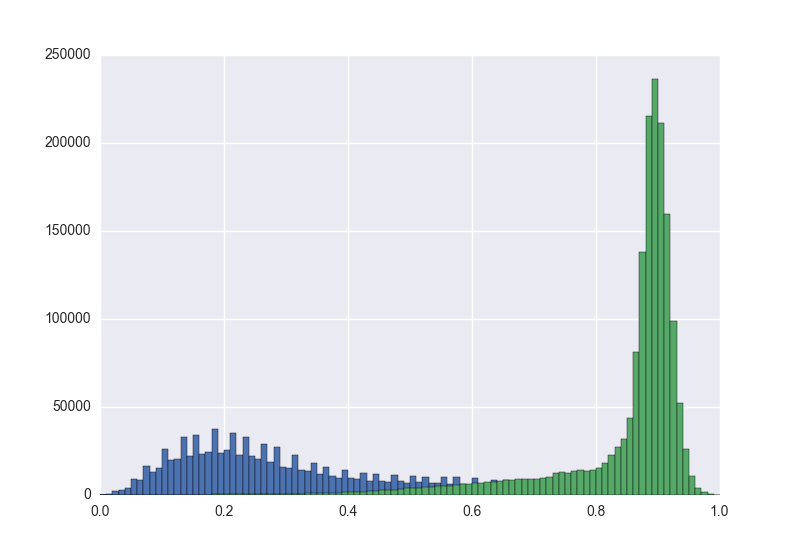
\includegraphics[width=0.8\textwidth]{Images/inverted_hist.png}	
	\caption{Comparison of the histogram of a real mammogram (blue) against a synthetic mammogram (green). The distribution of intensities are radically different from one another.}
\end{figure}

\clearpage
\begin{figure}[H]
	\centering
	\subfigure{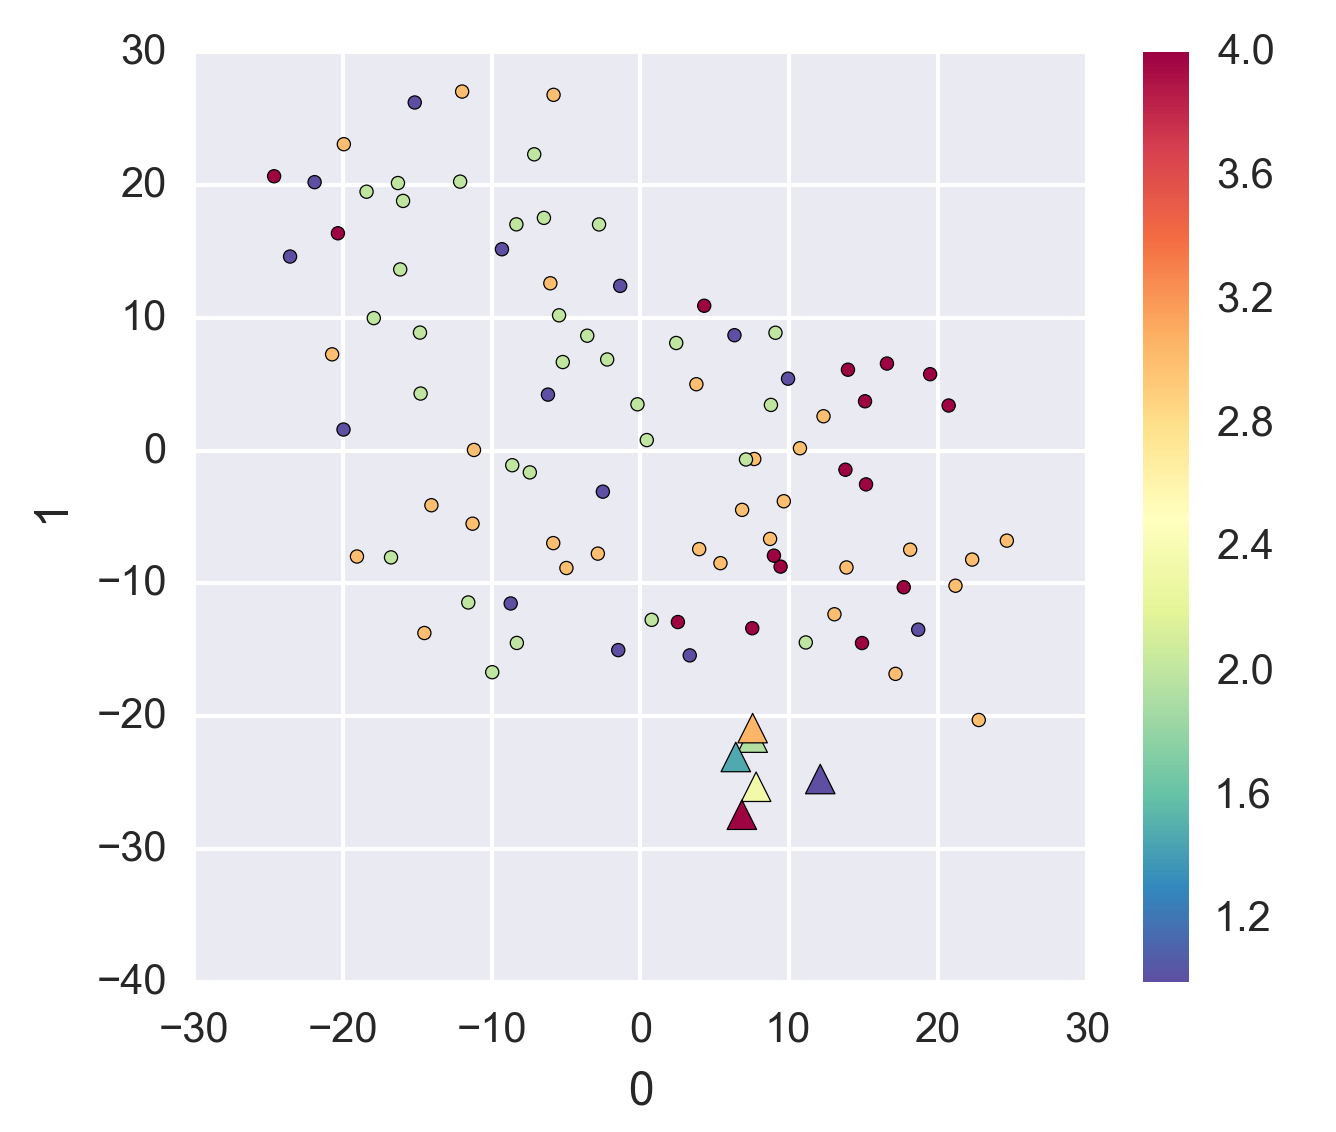
\includegraphics[width=0.49\textwidth]{figures/mappings/intensity_SNE_mapping_2d.png}}
	\subfigure{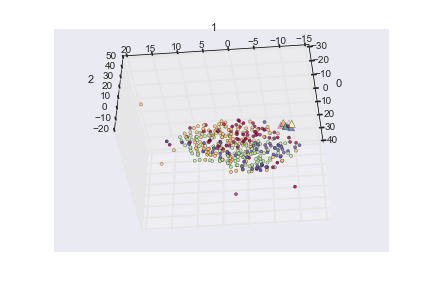
\includegraphics[width=0.49\textwidth]{figures/mappings/intensity_SNE_mapping_3d.png}}
	\caption{2D \& 3D projections of the intensity feature space produced by the t-SNE algorithm with a learning rate of 300 and perplexity of 30.}\label{fig:intensity_SNE_mapping}
\end{figure}

\begin{figure}[H]
	\centering
	\subfigure{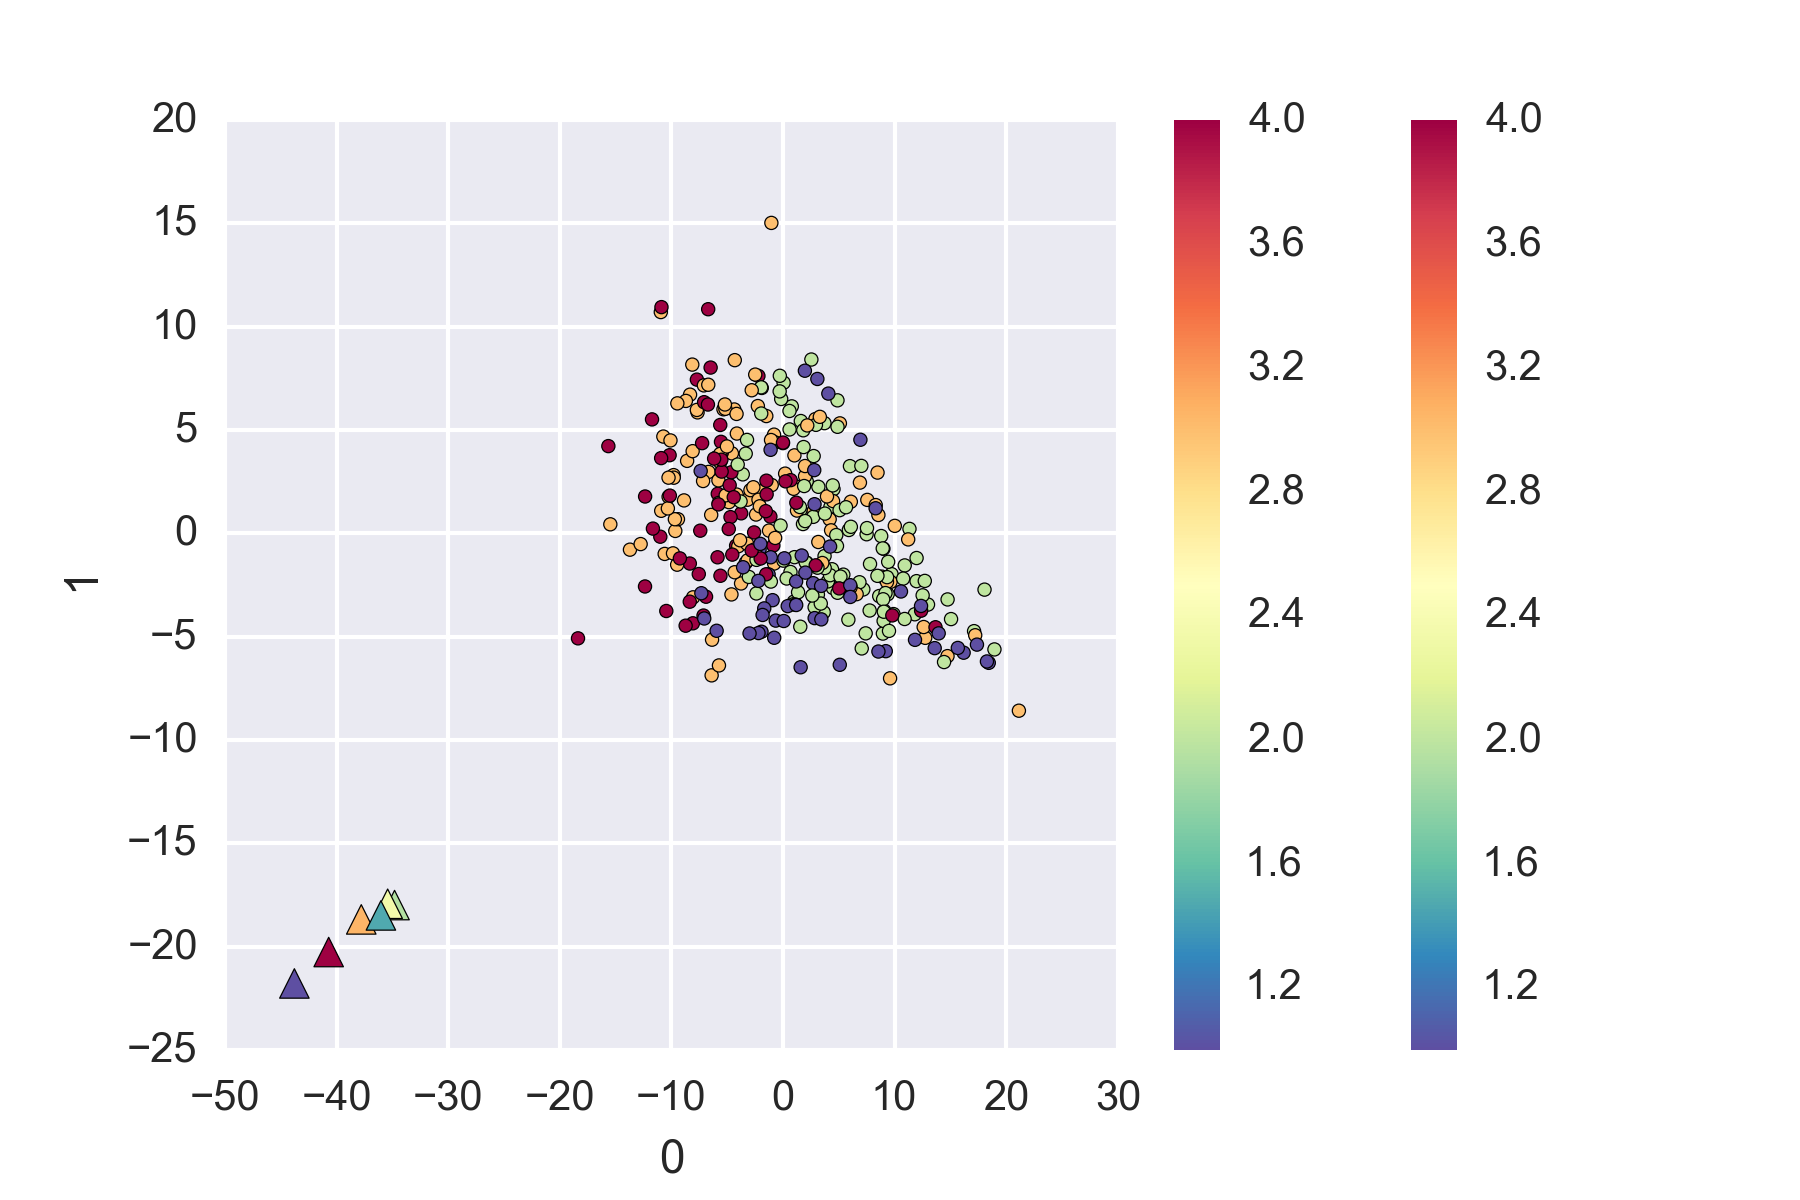
\includegraphics[width=0.49\textwidth]{figures/mappings/intensity_iso_mapping_2d.png}}
	\subfigure{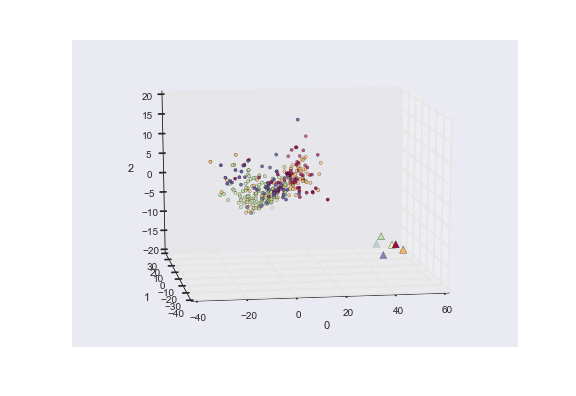
\includegraphics[width=0.49\textwidth]{figures/mappings/intensity_iso_mapping_3d.png}}
	\caption{2D \& 3D projections of the intensity feature space generated from blobs produced by the Isomap algorithm with 50 neighbours.}\label{fig:intensity_iso_mapping}
\end{figure}

\begin{figure}[H]
	\centering
	\subfigure{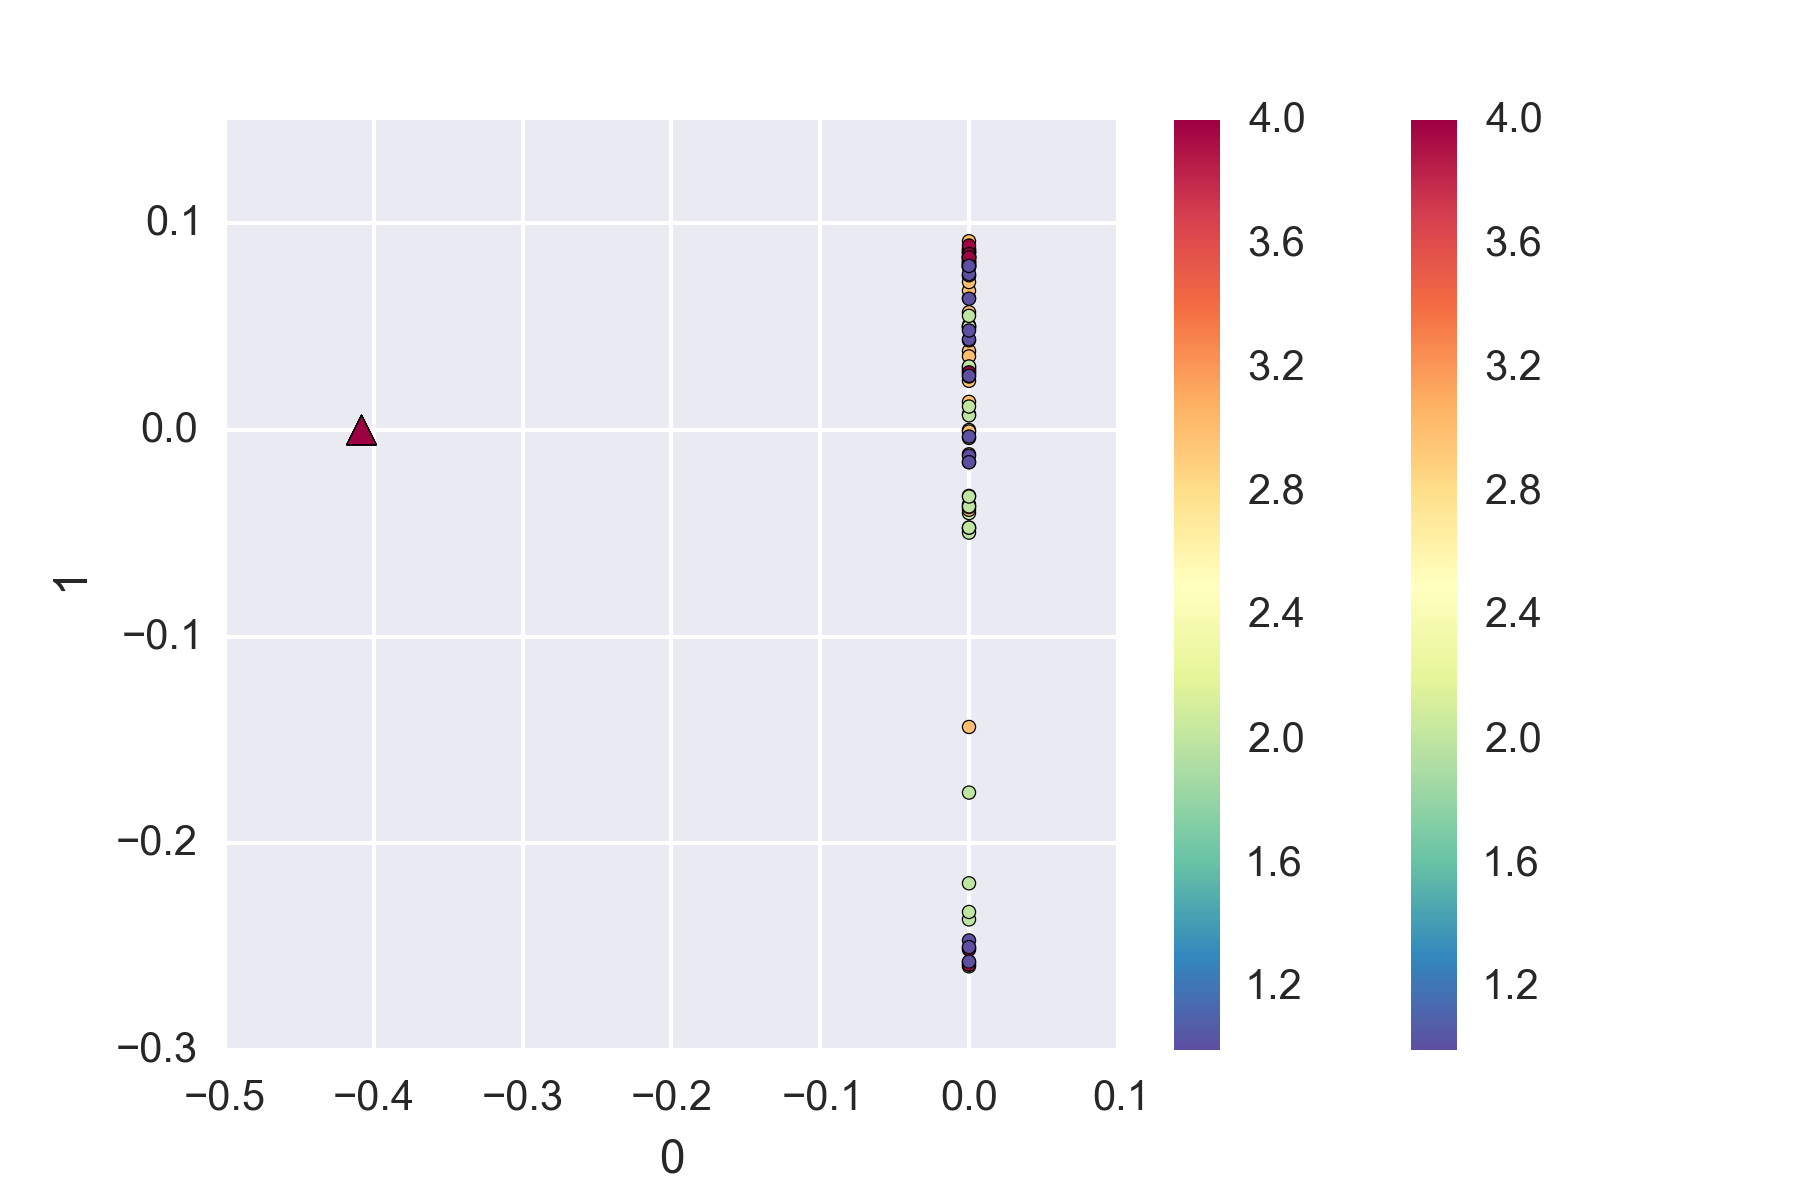
\includegraphics[width=0.49\textwidth]{figures/mappings/intensity_lle_mapping_2d.png}}
	\subfigure{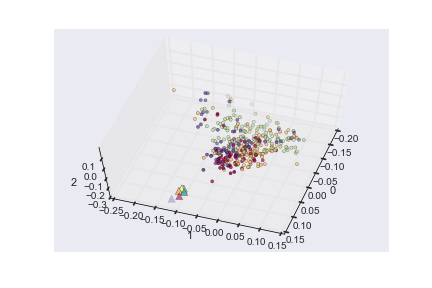
\includegraphics[width=0.49\textwidth]{figures/mappings/intensity_lle_mapping_3d.png}}
	\caption{2D \& 3D projections of the intensity feature space generated from blobs produced by the LLE algorithm with 50 neighbours.}\label{fig:intensity_LLE_mapping}
\end{figure}
\clearpage

\clearpage
\begin{figure}[H]
	\centering
	\subfigure{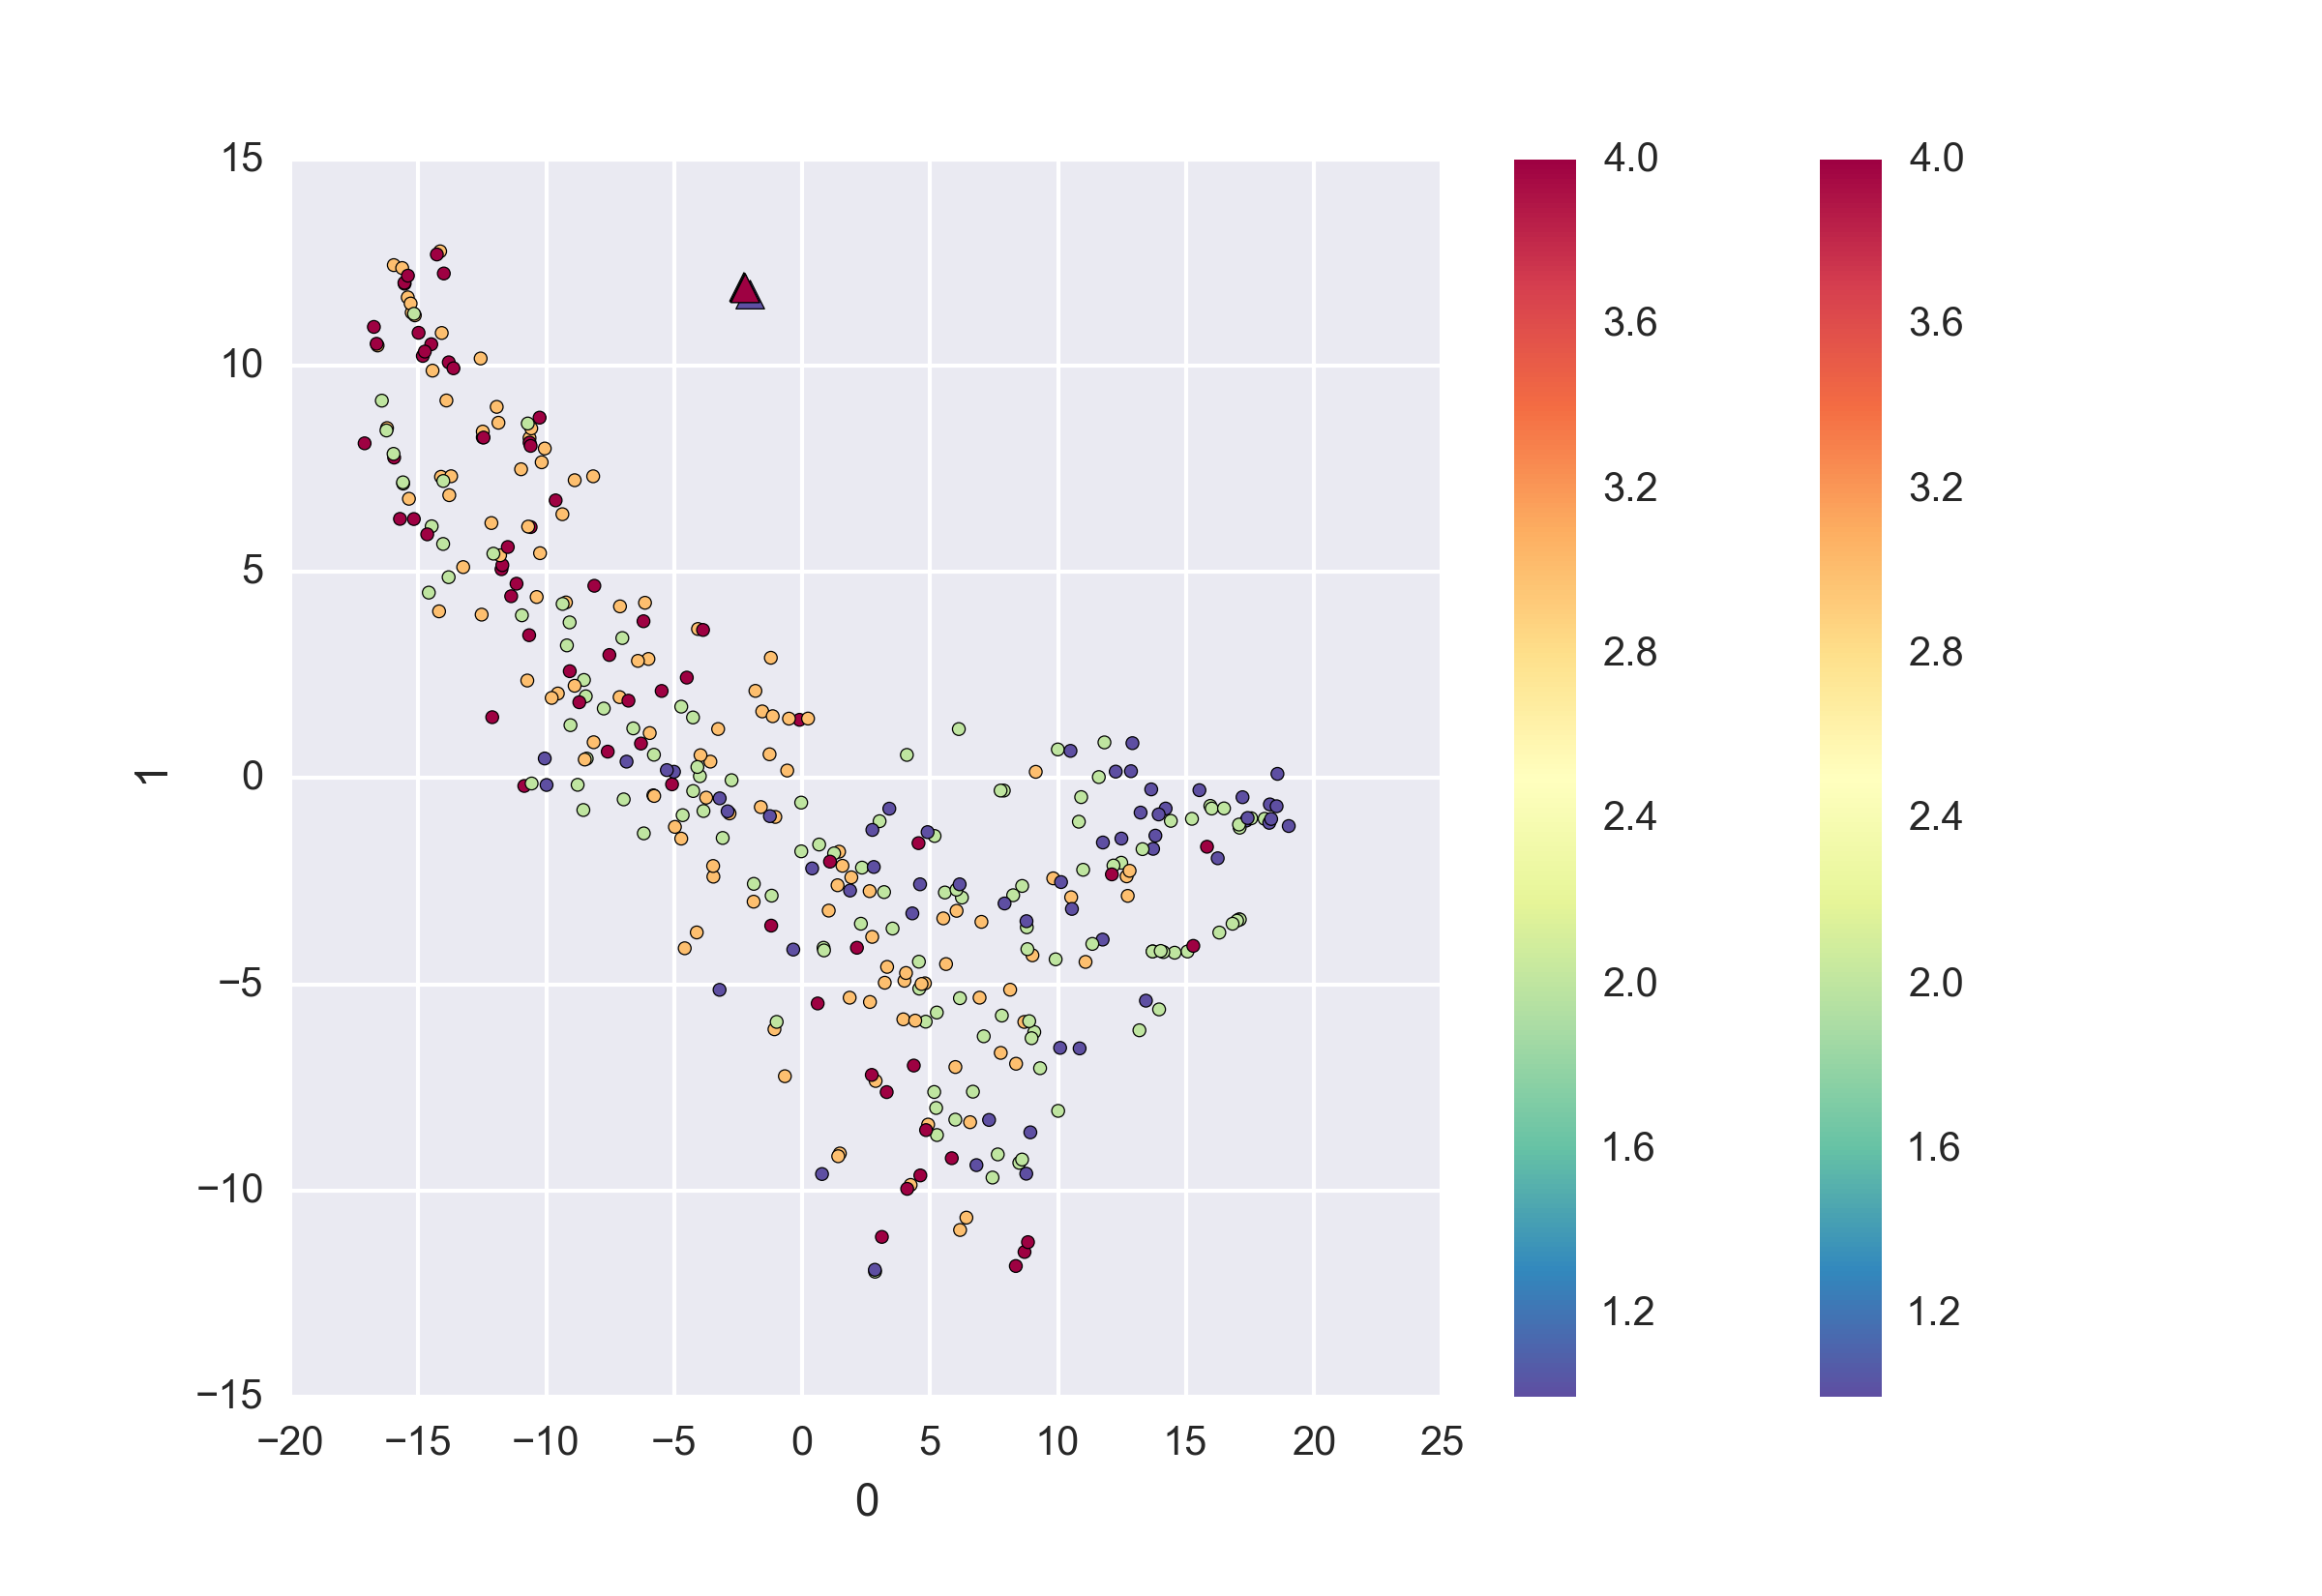
\includegraphics[width=0.49\textwidth]{figures/mappings/texture_SNE_mapping_2d.png}}
	\subfigure{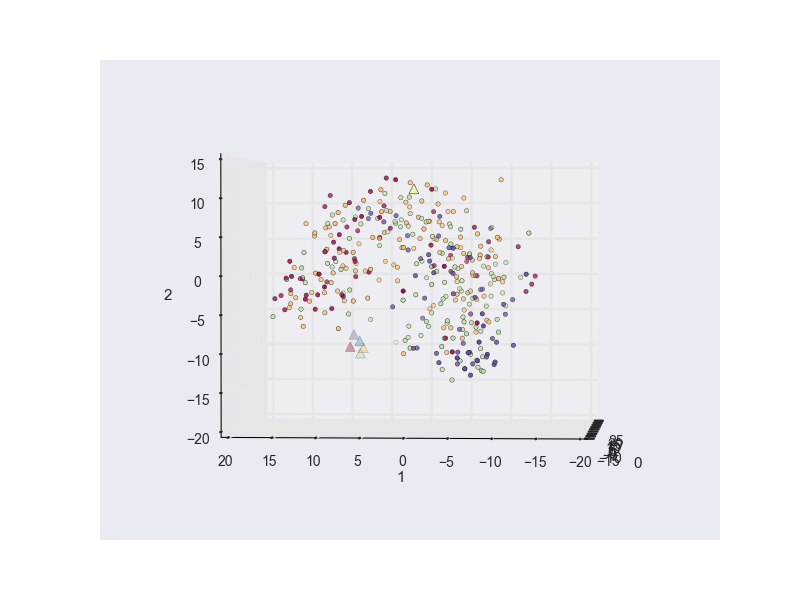
\includegraphics[width=0.49\textwidth]{figures/mappings/texture_SNE_mapping_3d.png}}
	\caption{2D \& 3D projections of the texture feature space generated from blobs generated from blobs produced by the t-SNE algorithm with a learning rate of 300 and perplexity of 30.}\label{fig:texture_SNE_mapping}
\end{figure}

\begin{figure}[H]
	\centering
	\subfigure{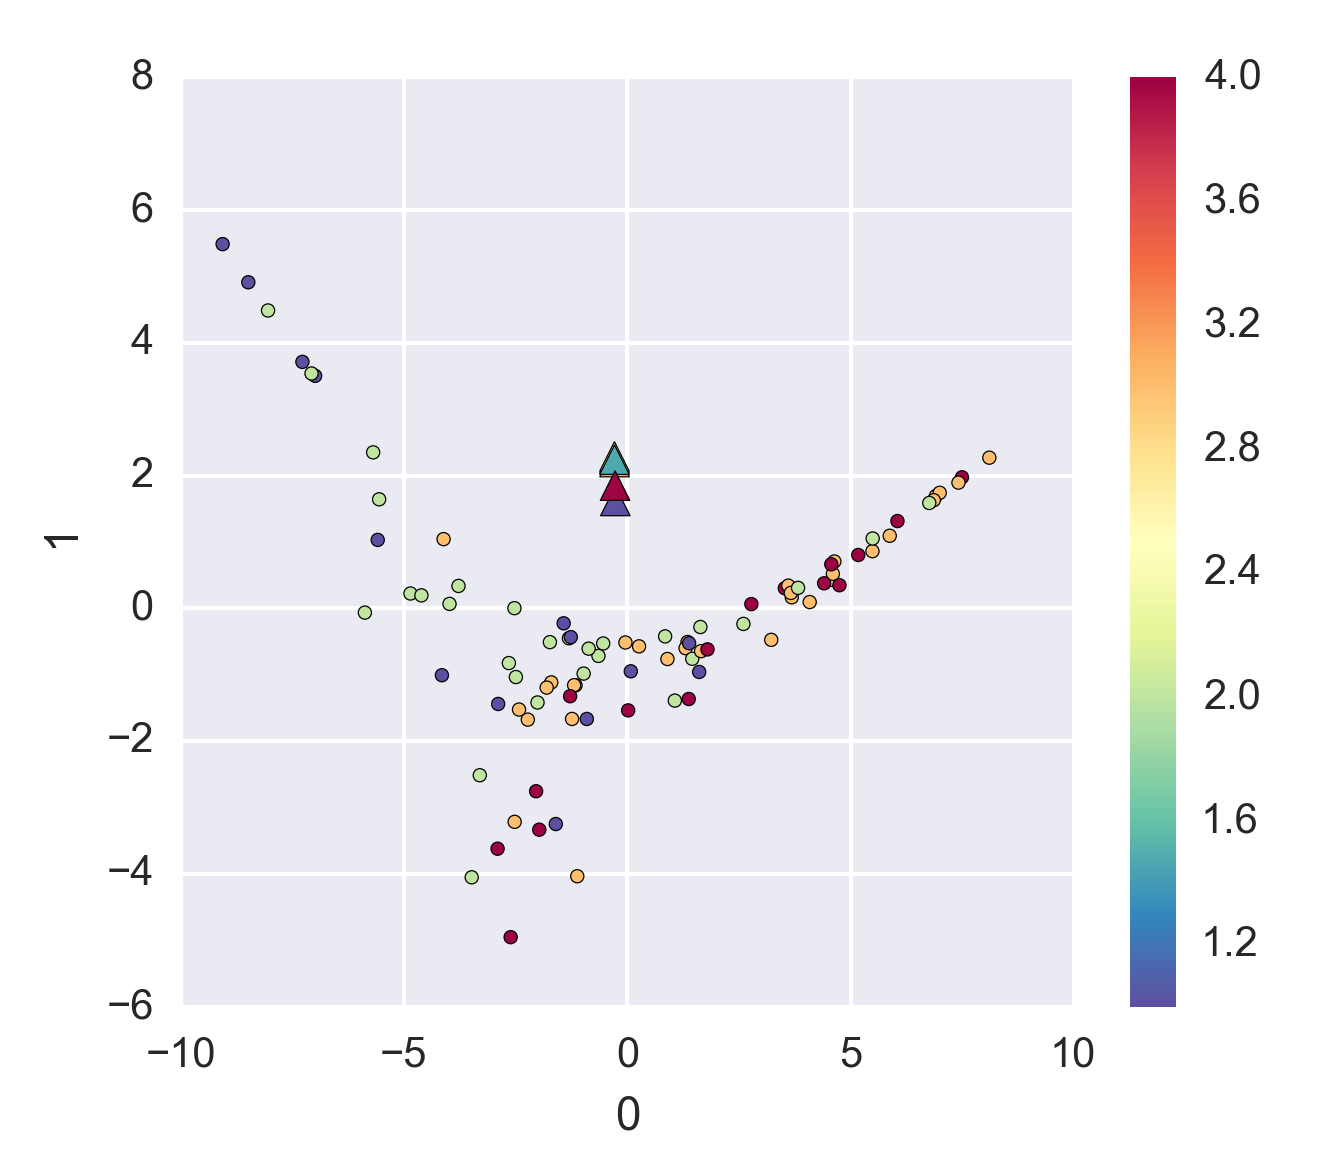
\includegraphics[width=0.49\textwidth]{figures/mappings/texture_iso_mapping_2d.png}}
	\subfigure{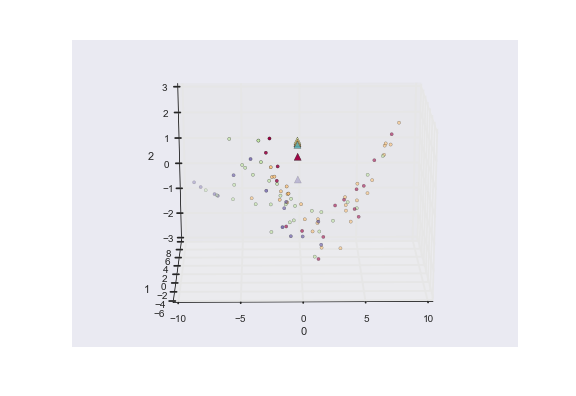
\includegraphics[width=0.49\textwidth]{figures/mappings/texture_iso_mapping_3d.png}}
	\caption{2D \& 3D projections of the texture feature space generated from blobs produced by the Isomap algorithm with 50 neighbours.}\label{fig:texture_iso_mapping}
\end{figure}

\begin{figure}[H]
	\centering
	\subfigure{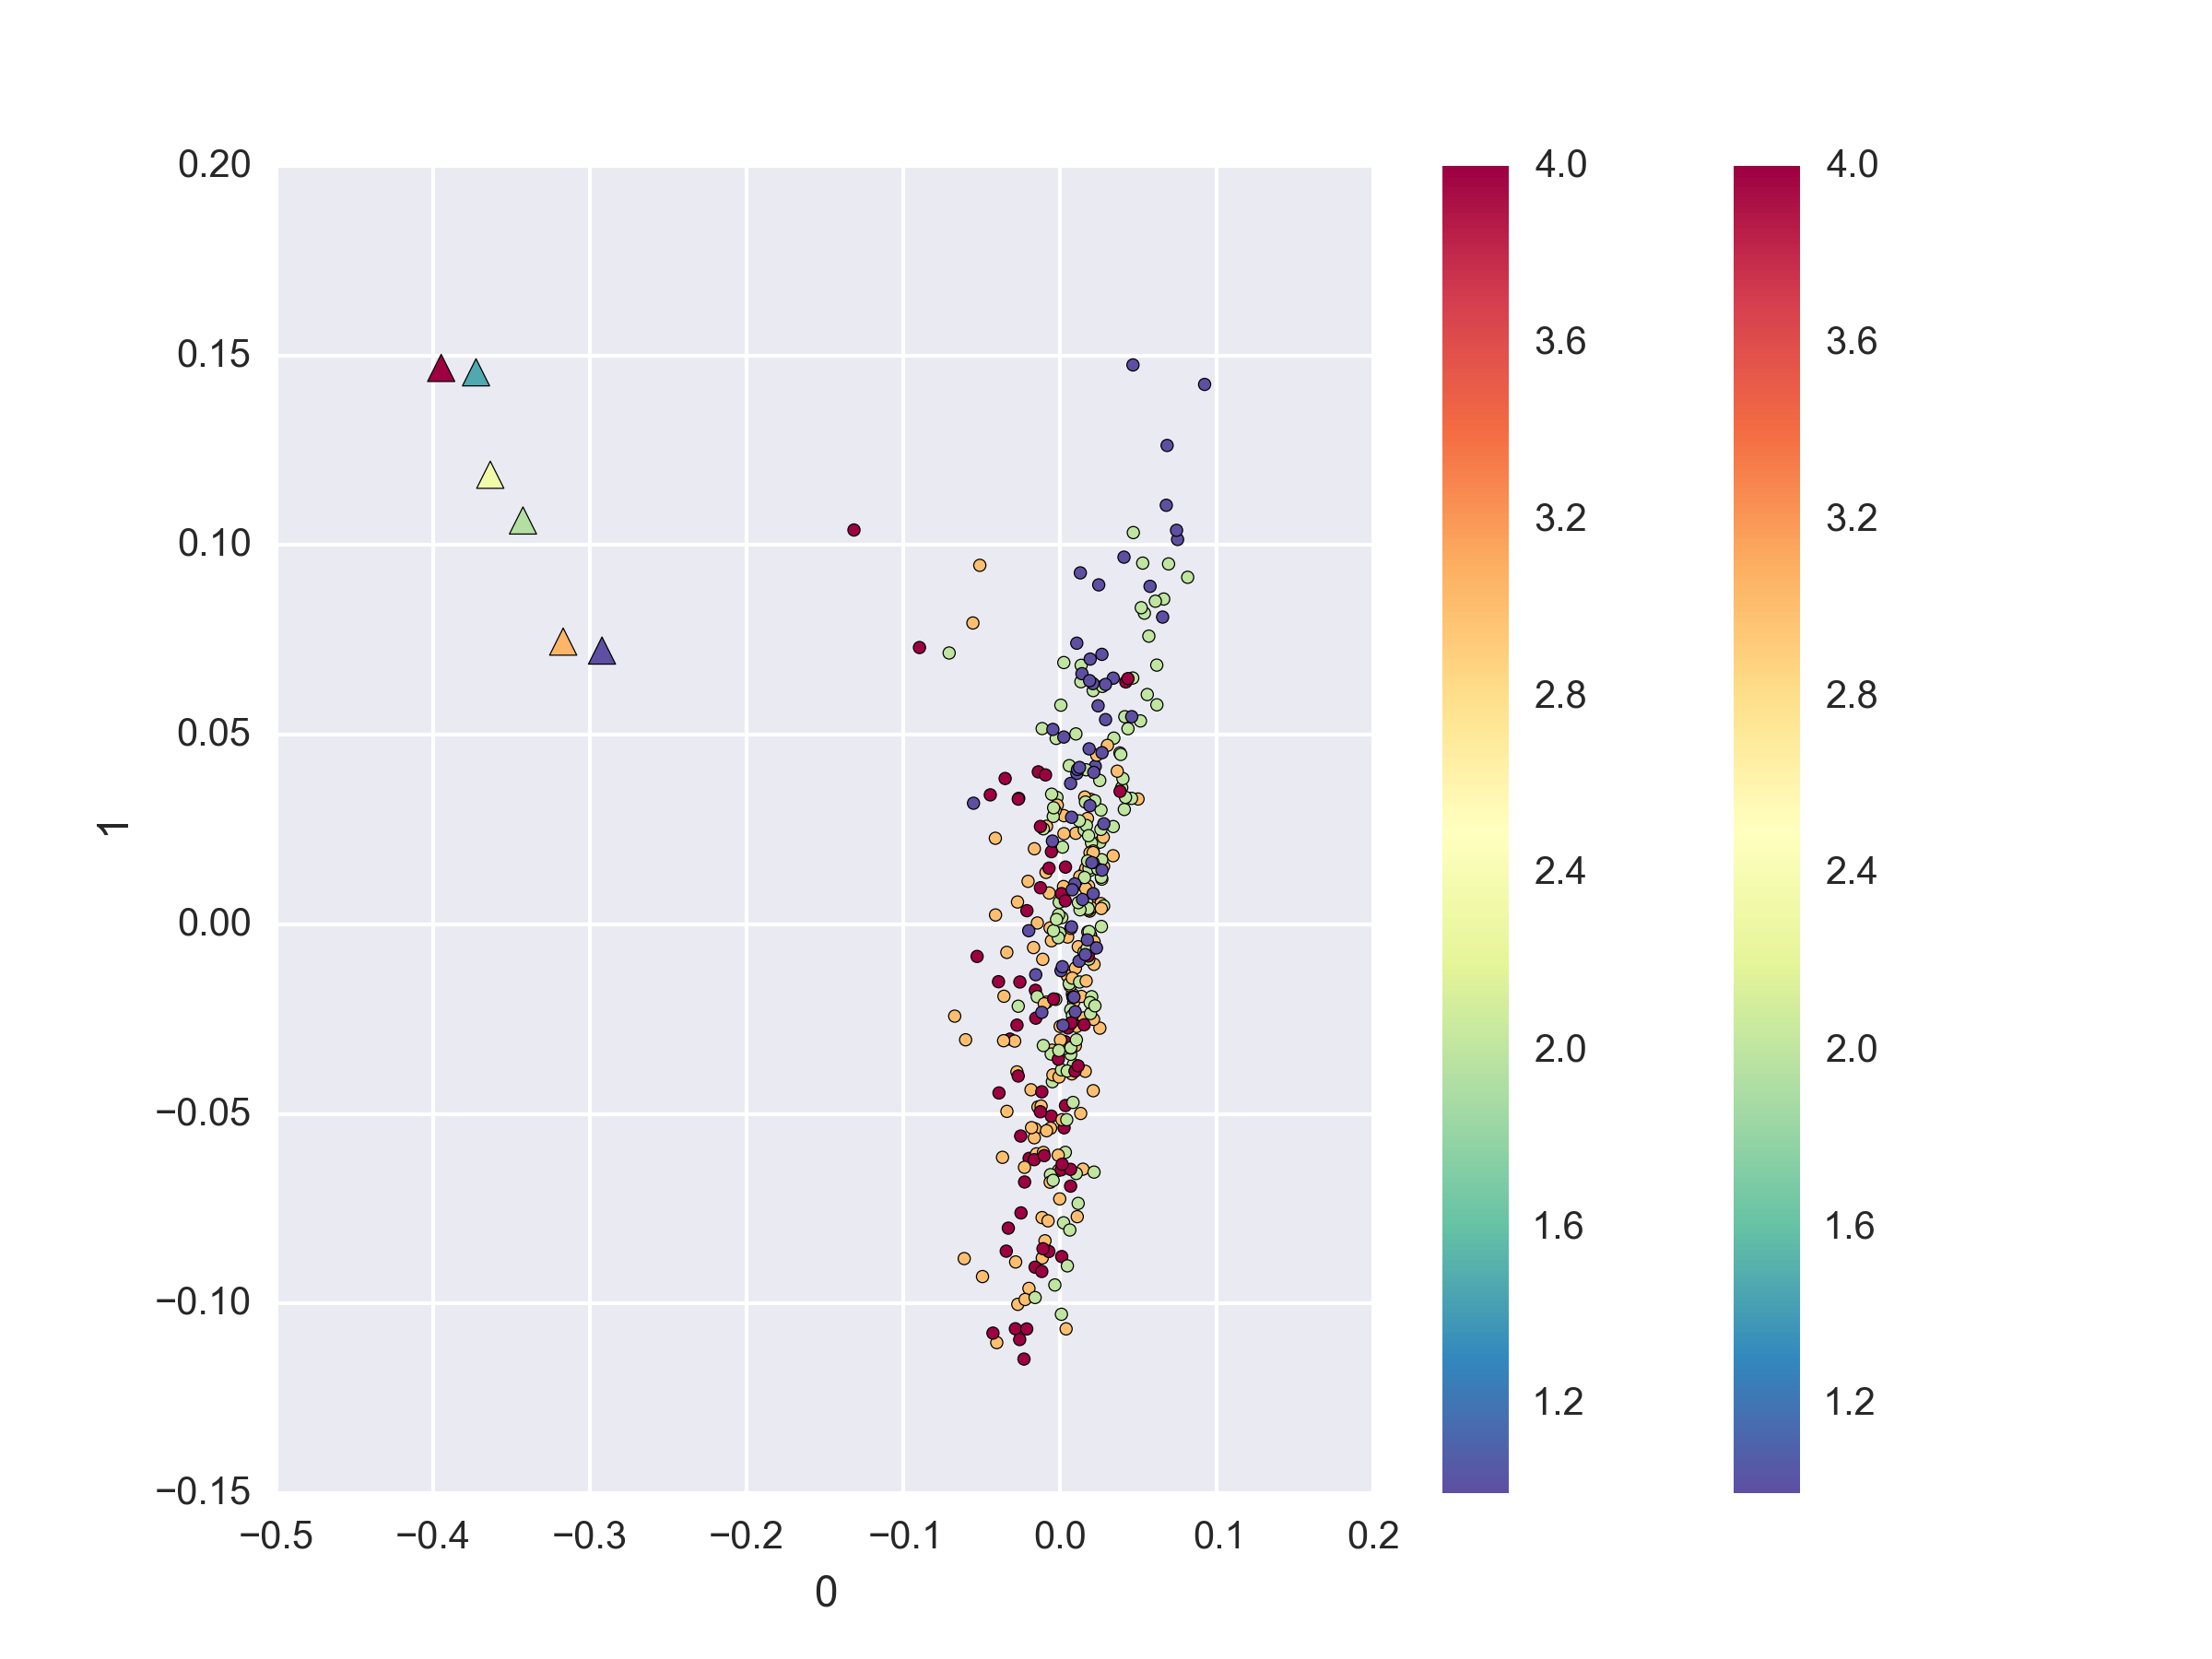
\includegraphics[width=0.49\textwidth]{figures/mappings/texture_lle_mapping_2d.png}}
	\subfigure{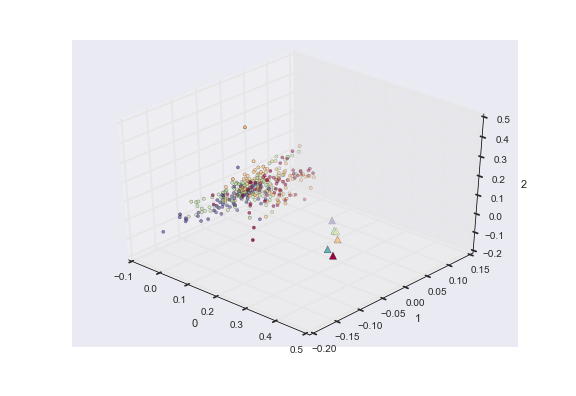
\includegraphics[width=0.49\textwidth]{figures/mappings/texture_lle_mapping_3d.png}}
	\caption{2D \& 3D projections of the texture feature space generated from blobs produced by the LLE algorithm with 50 neighbours.}\label{fig:texture_LLE_mapping}
\end{figure}
\clearpage

\section{Quality Assessment of Visualisations}
Two different kinds of quality measure derived from the co-ranking matrix were computed for each of the visualisations shown in the preceding section of this document. These quality metrics were Trustworthiness \& continuity and the local continuity meta-criteria.


\clearpage
\begin{figure}[H]
	\centering
	\subfigure{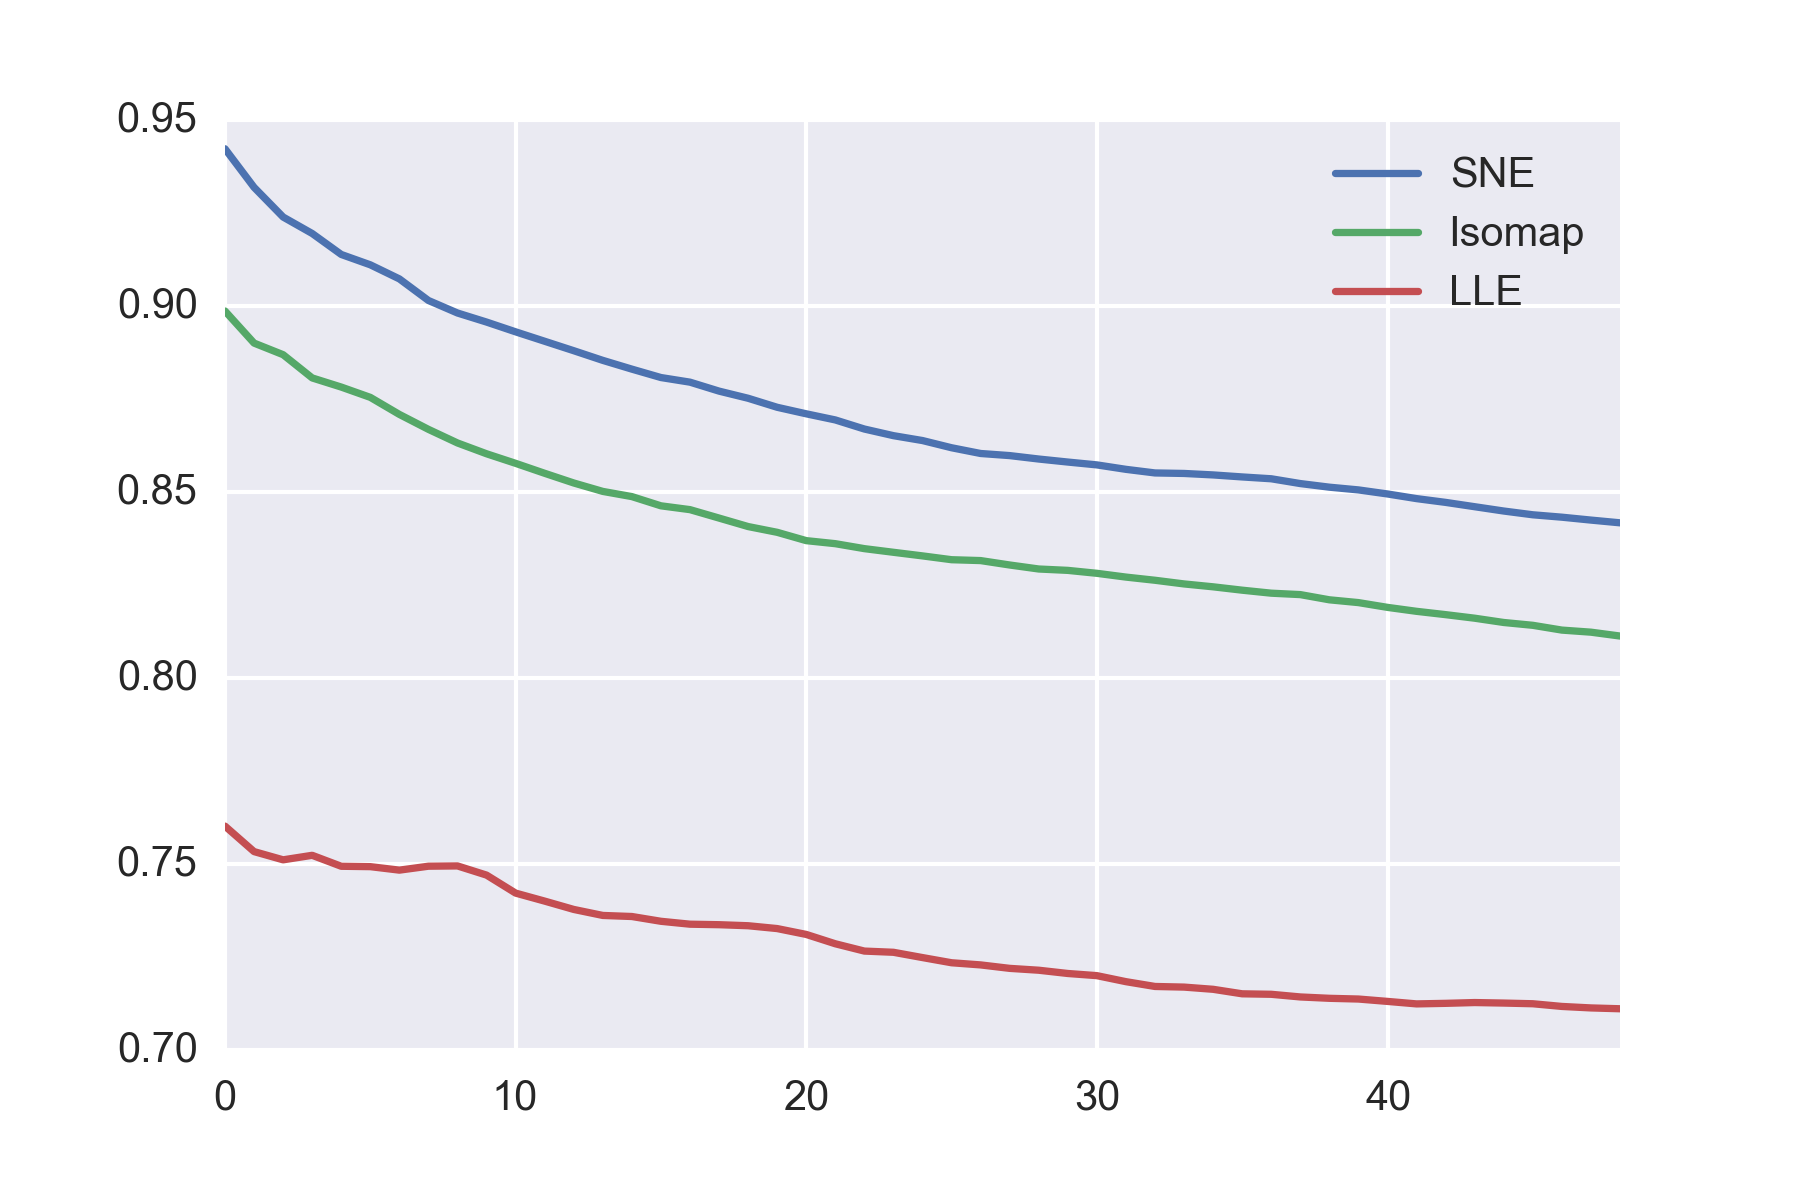
\includegraphics[width=0.49\textwidth]{figures/quality_measures/blob_trustworthiness_2d.png}}
	\subfigure{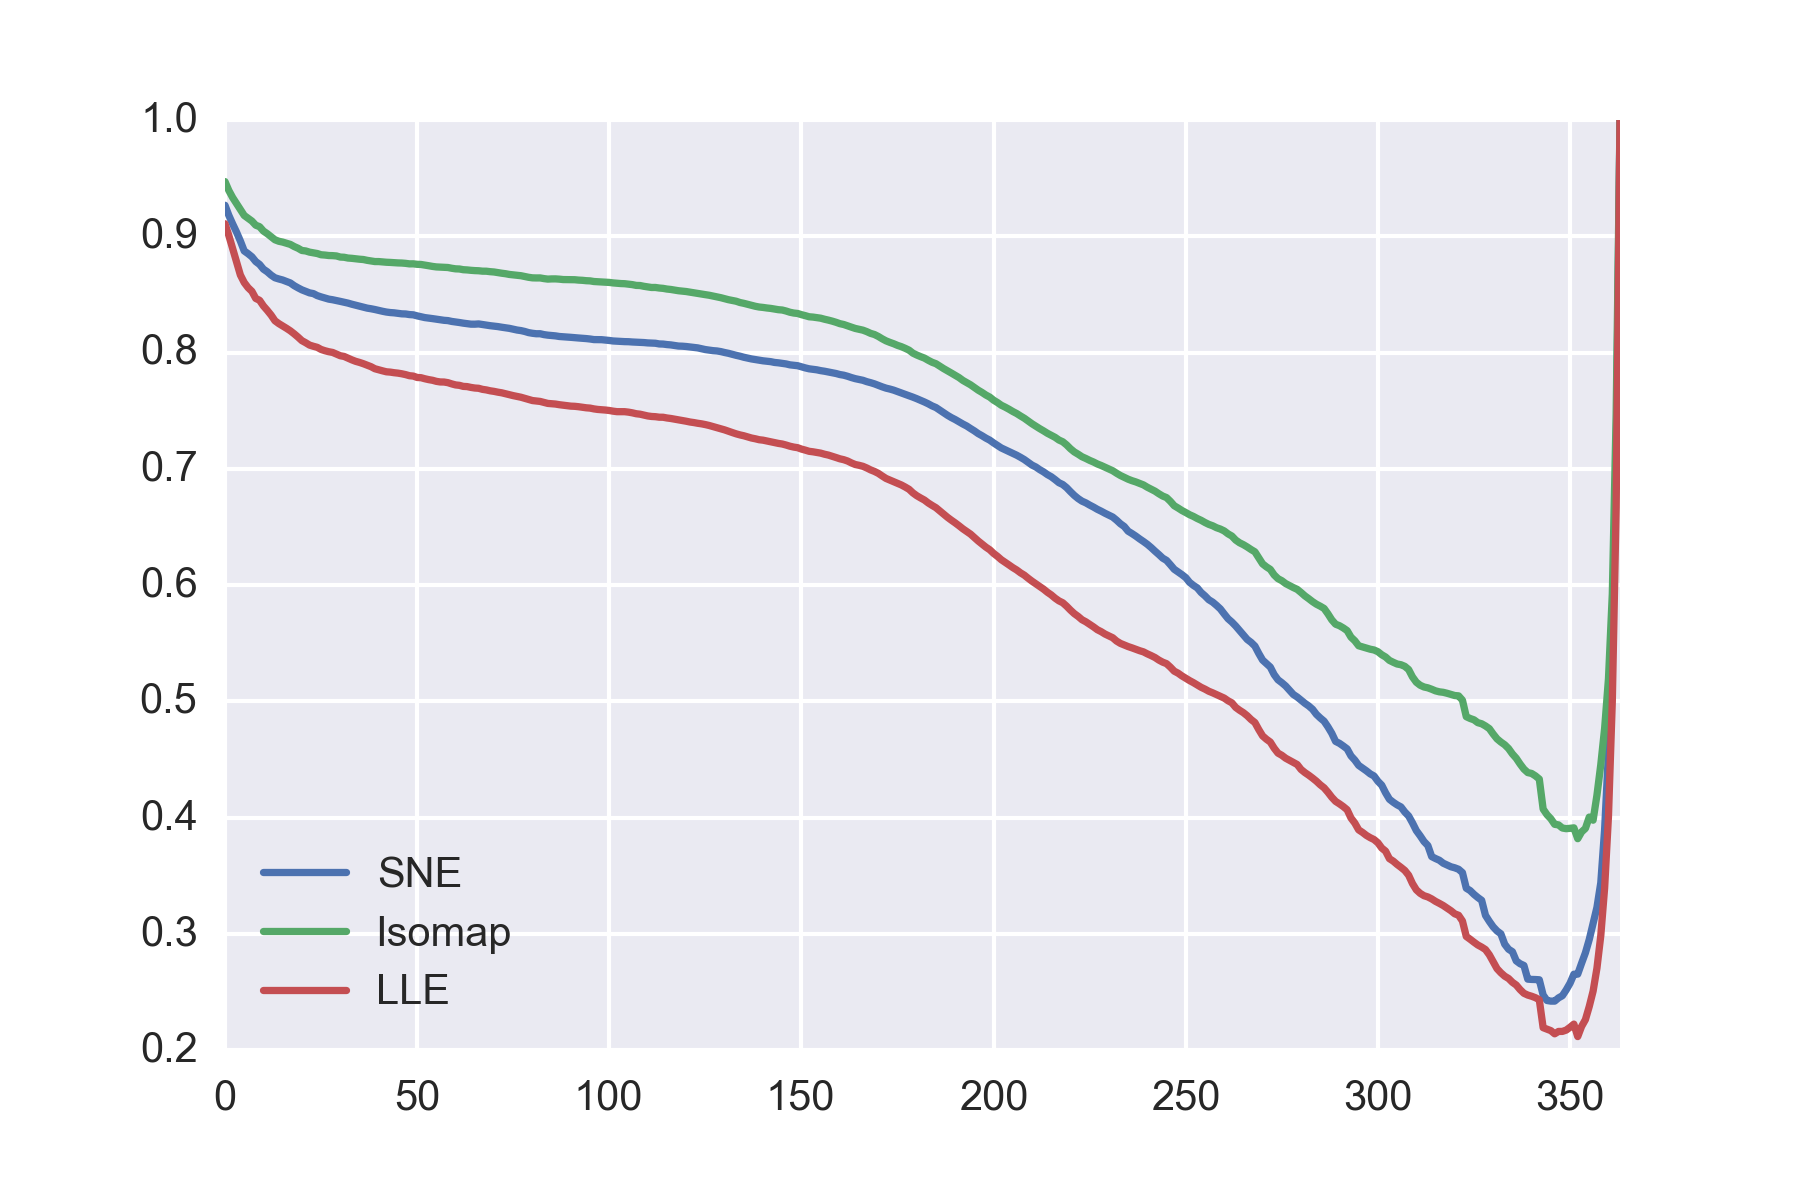
\includegraphics[width=0.49\textwidth]{figures/quality_measures/blob_continuity_2d.png}}
	\caption{Trustworthiness and continuity of the 2D projections produced from blob features.}\label{fig:TC_2d_blobs}
\end{figure}

\begin{figure}[H]
	\centering
	\subfigure{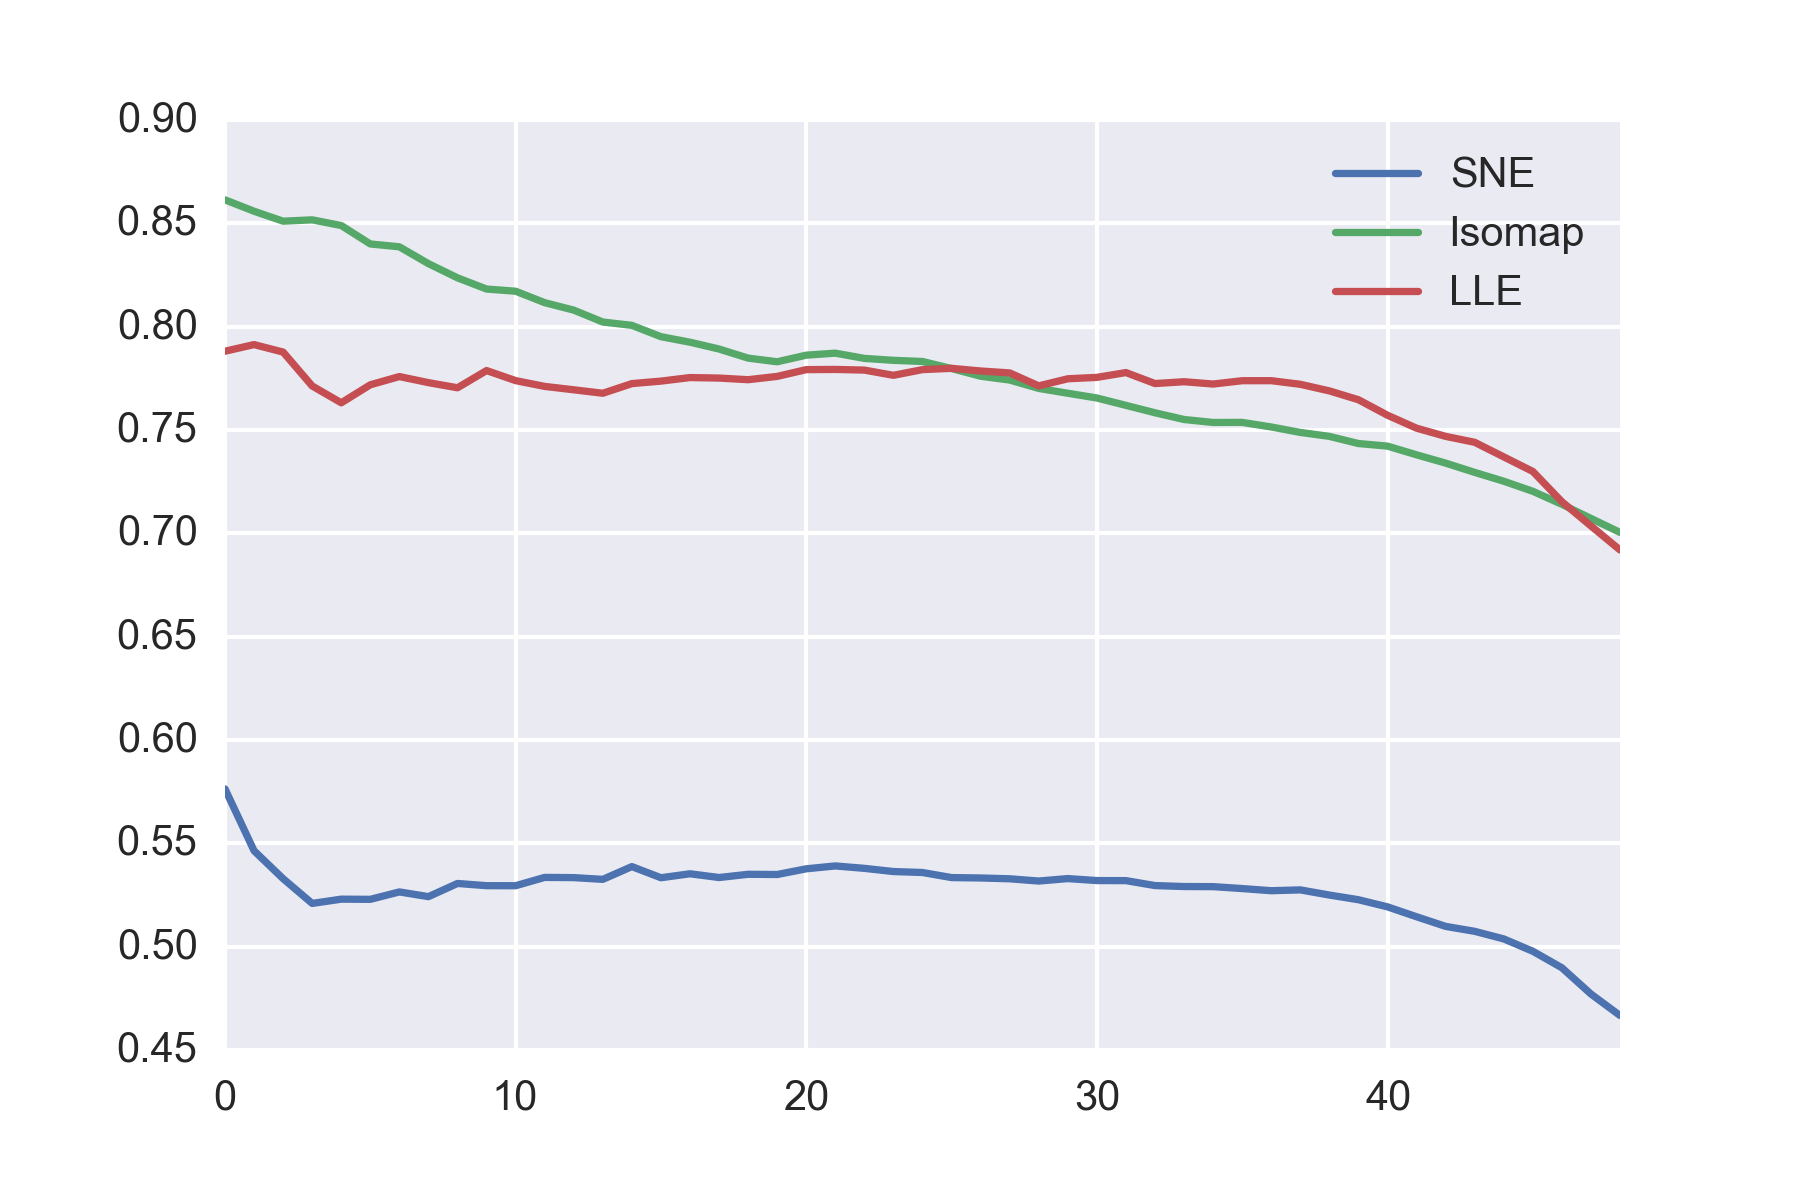
\includegraphics[width=0.49\textwidth]{figures/quality_measures/blob_trustworthiness_3d.png}}
	\subfigure{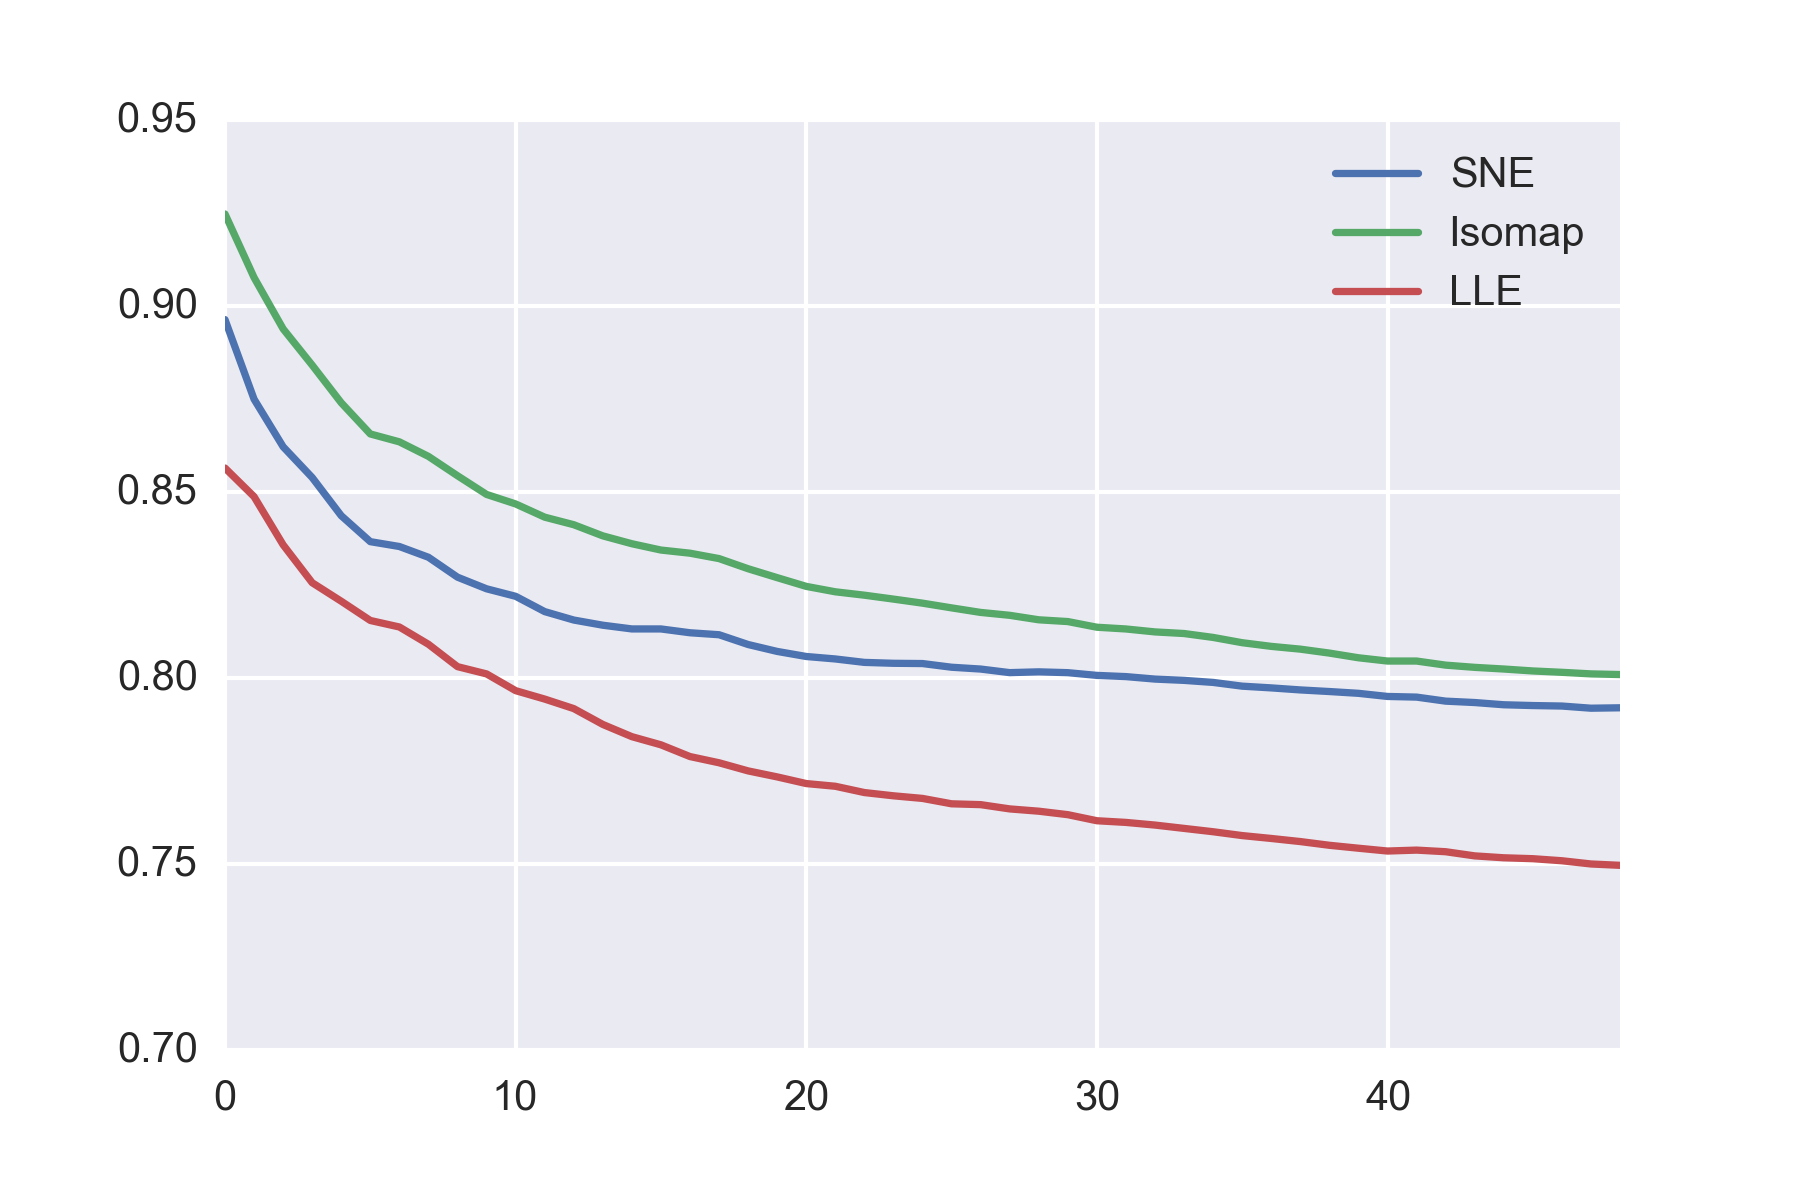
\includegraphics[width=0.49\textwidth]{figures/quality_measures/blob_continuity_3d.png}}
	\caption{Trustworthiness and continuity of the 3D projections produced from blob features.}\label{fig:TC_3d_blobs}
\end{figure}

\begin{figure}[H]
	\centering
	\subfigure{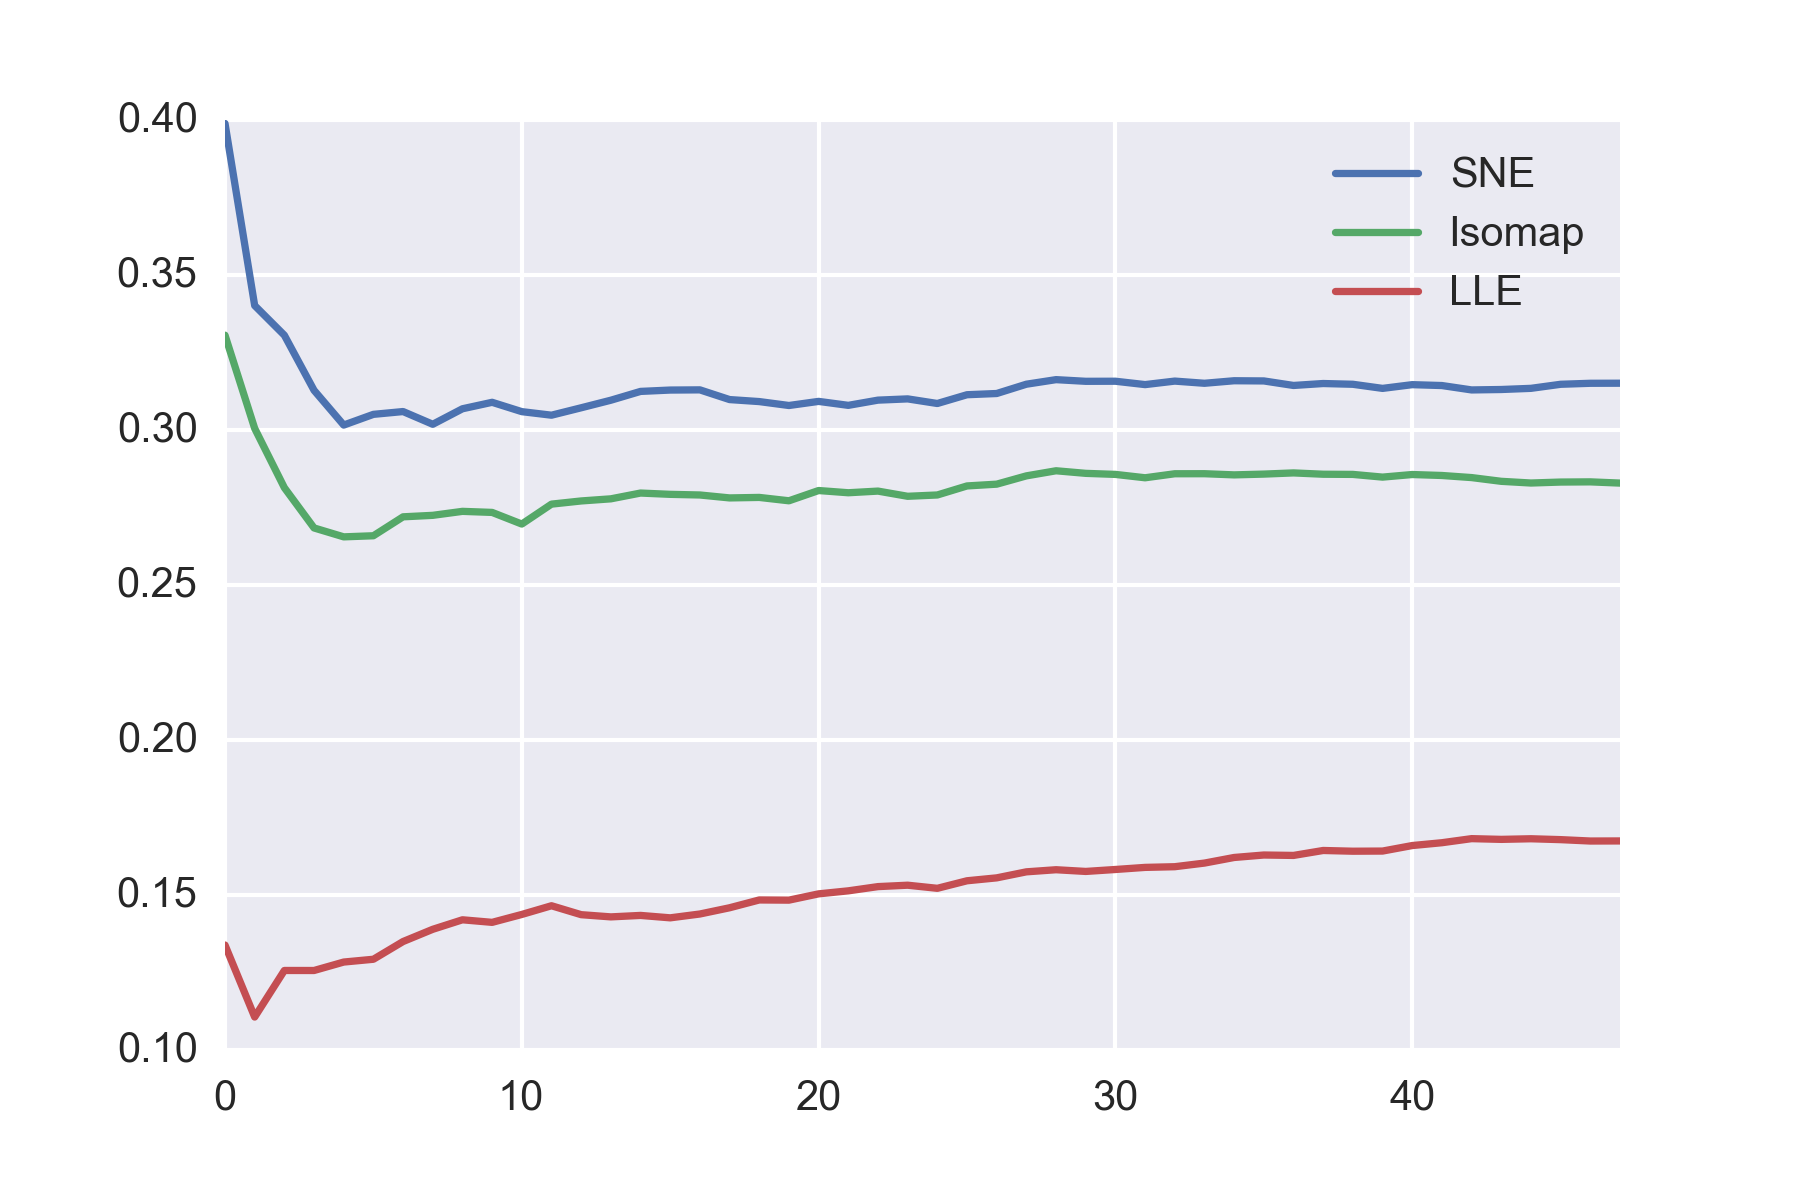
\includegraphics[width=0.49\textwidth]{figures/quality_measures/blob_lcmc_2d.png}}
	\subfigure{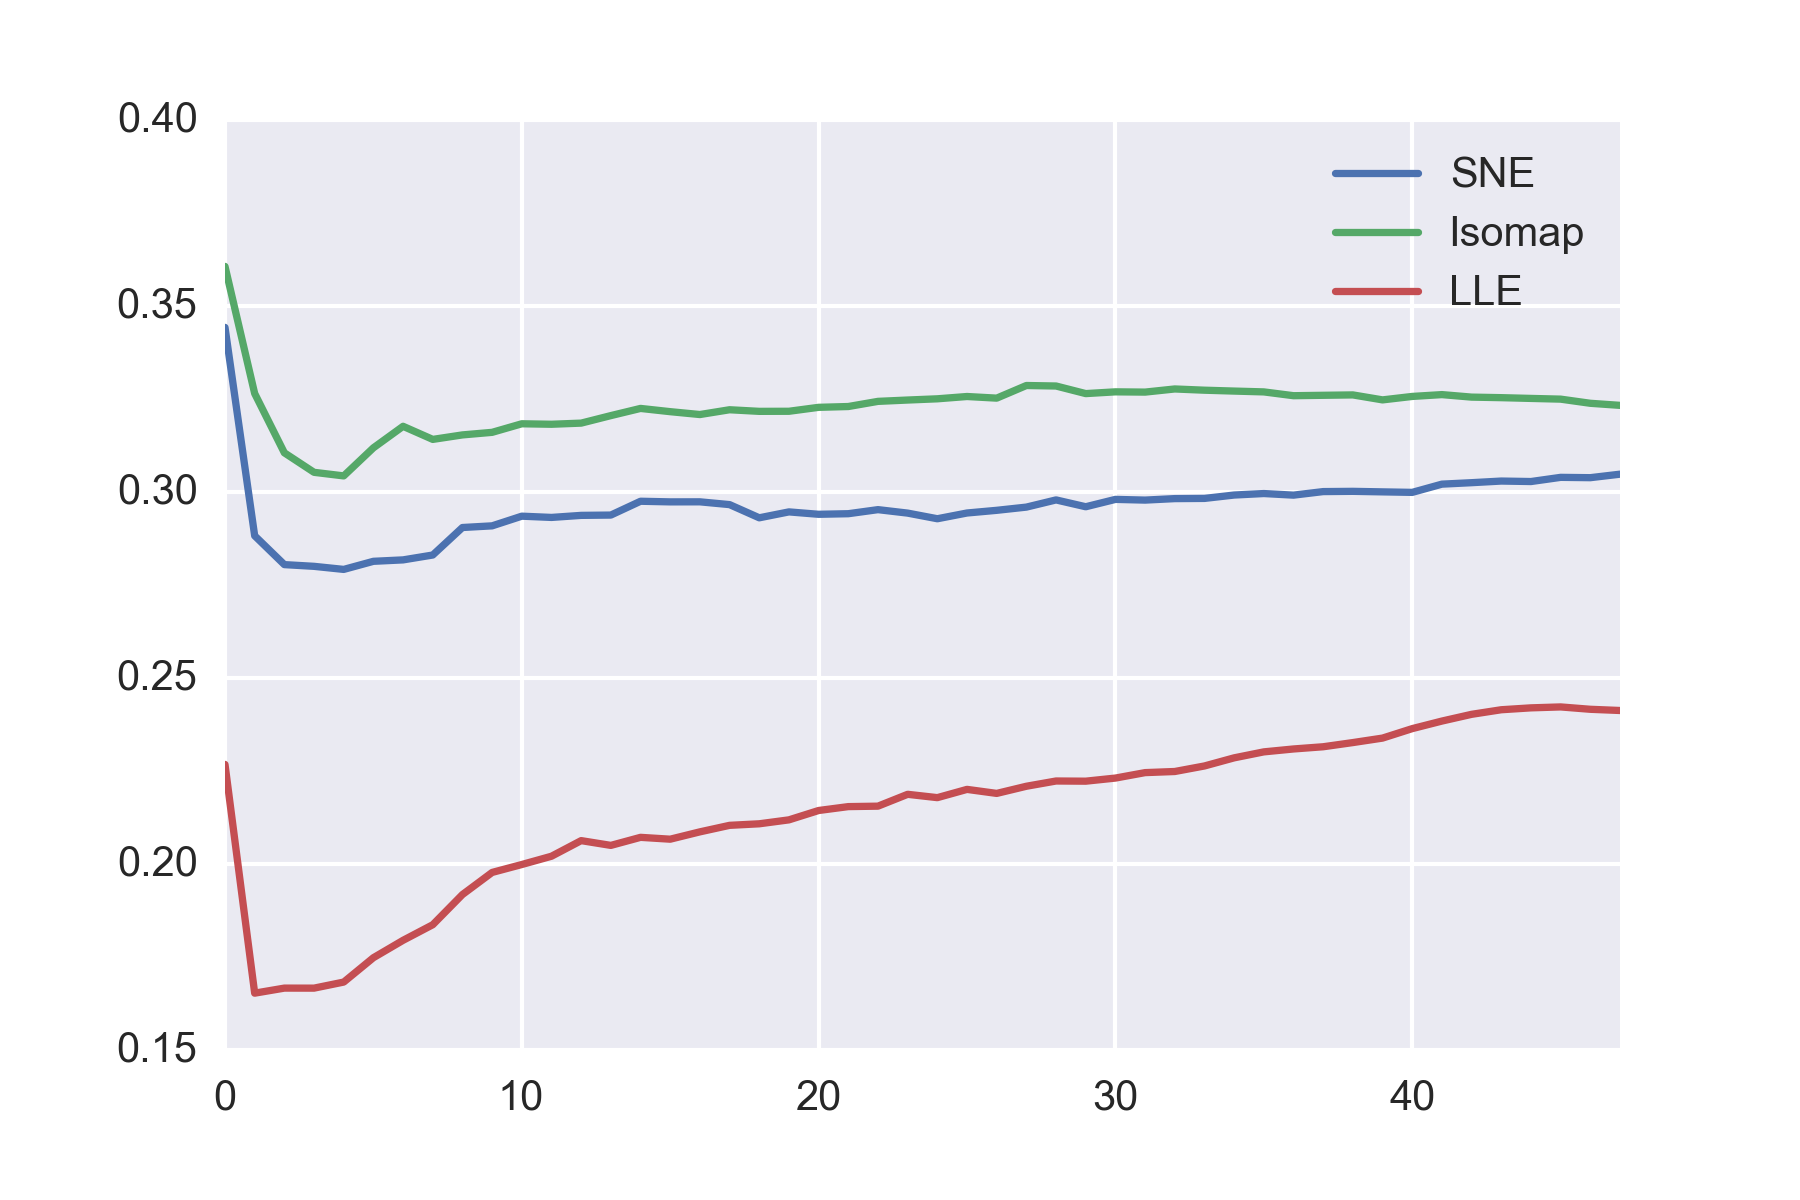
\includegraphics[width=0.49\textwidth]{figures/quality_measures/blob_lcmc_3d.png}}
	\caption{LCMC of both the 2D projection (left) and 3D projection (right) of the feature space for blobs.}\label{fig:LCMC_blobs}
\end{figure}

\clearpage
\begin{figure}[H]
	\centering
	\subfigure{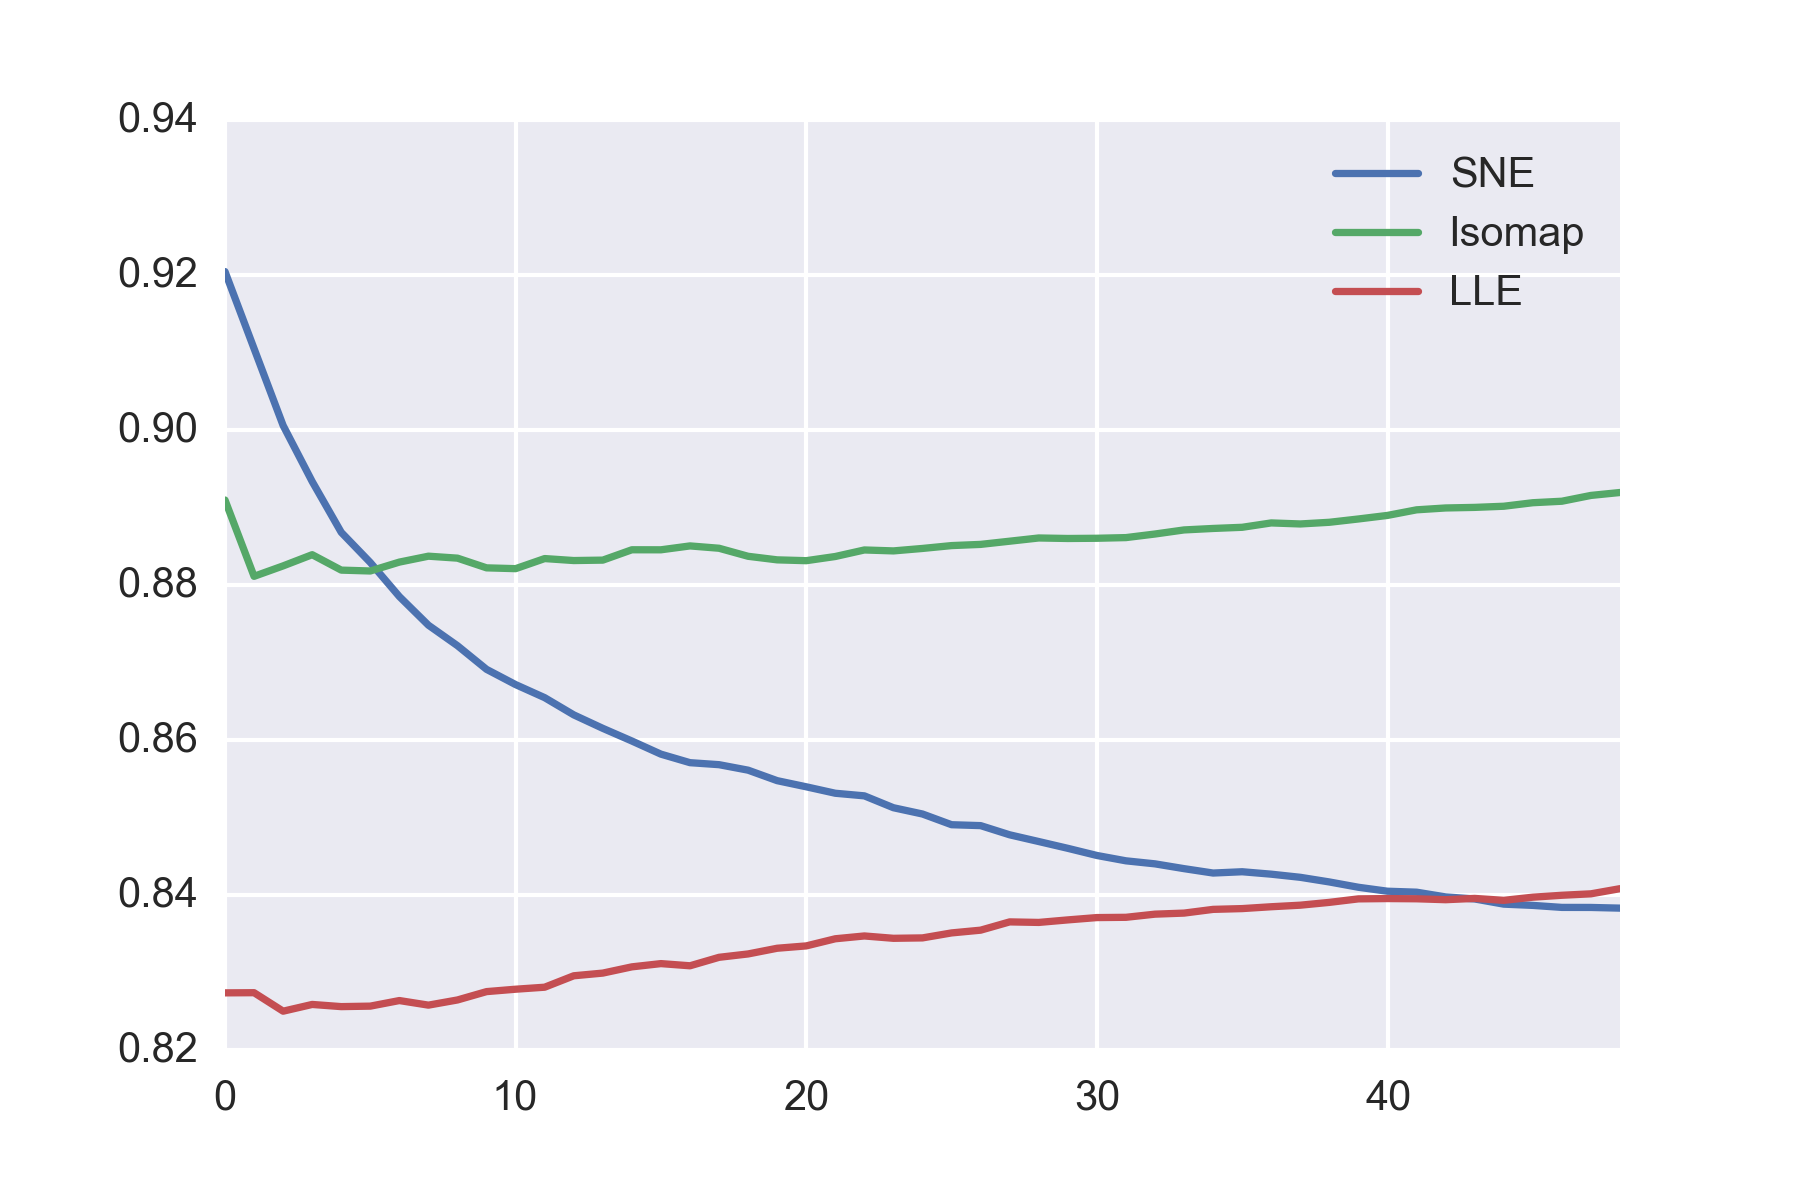
\includegraphics[width=0.49\textwidth]{figures/quality_measures/line_trustworthiness_2d.png}}
	\subfigure{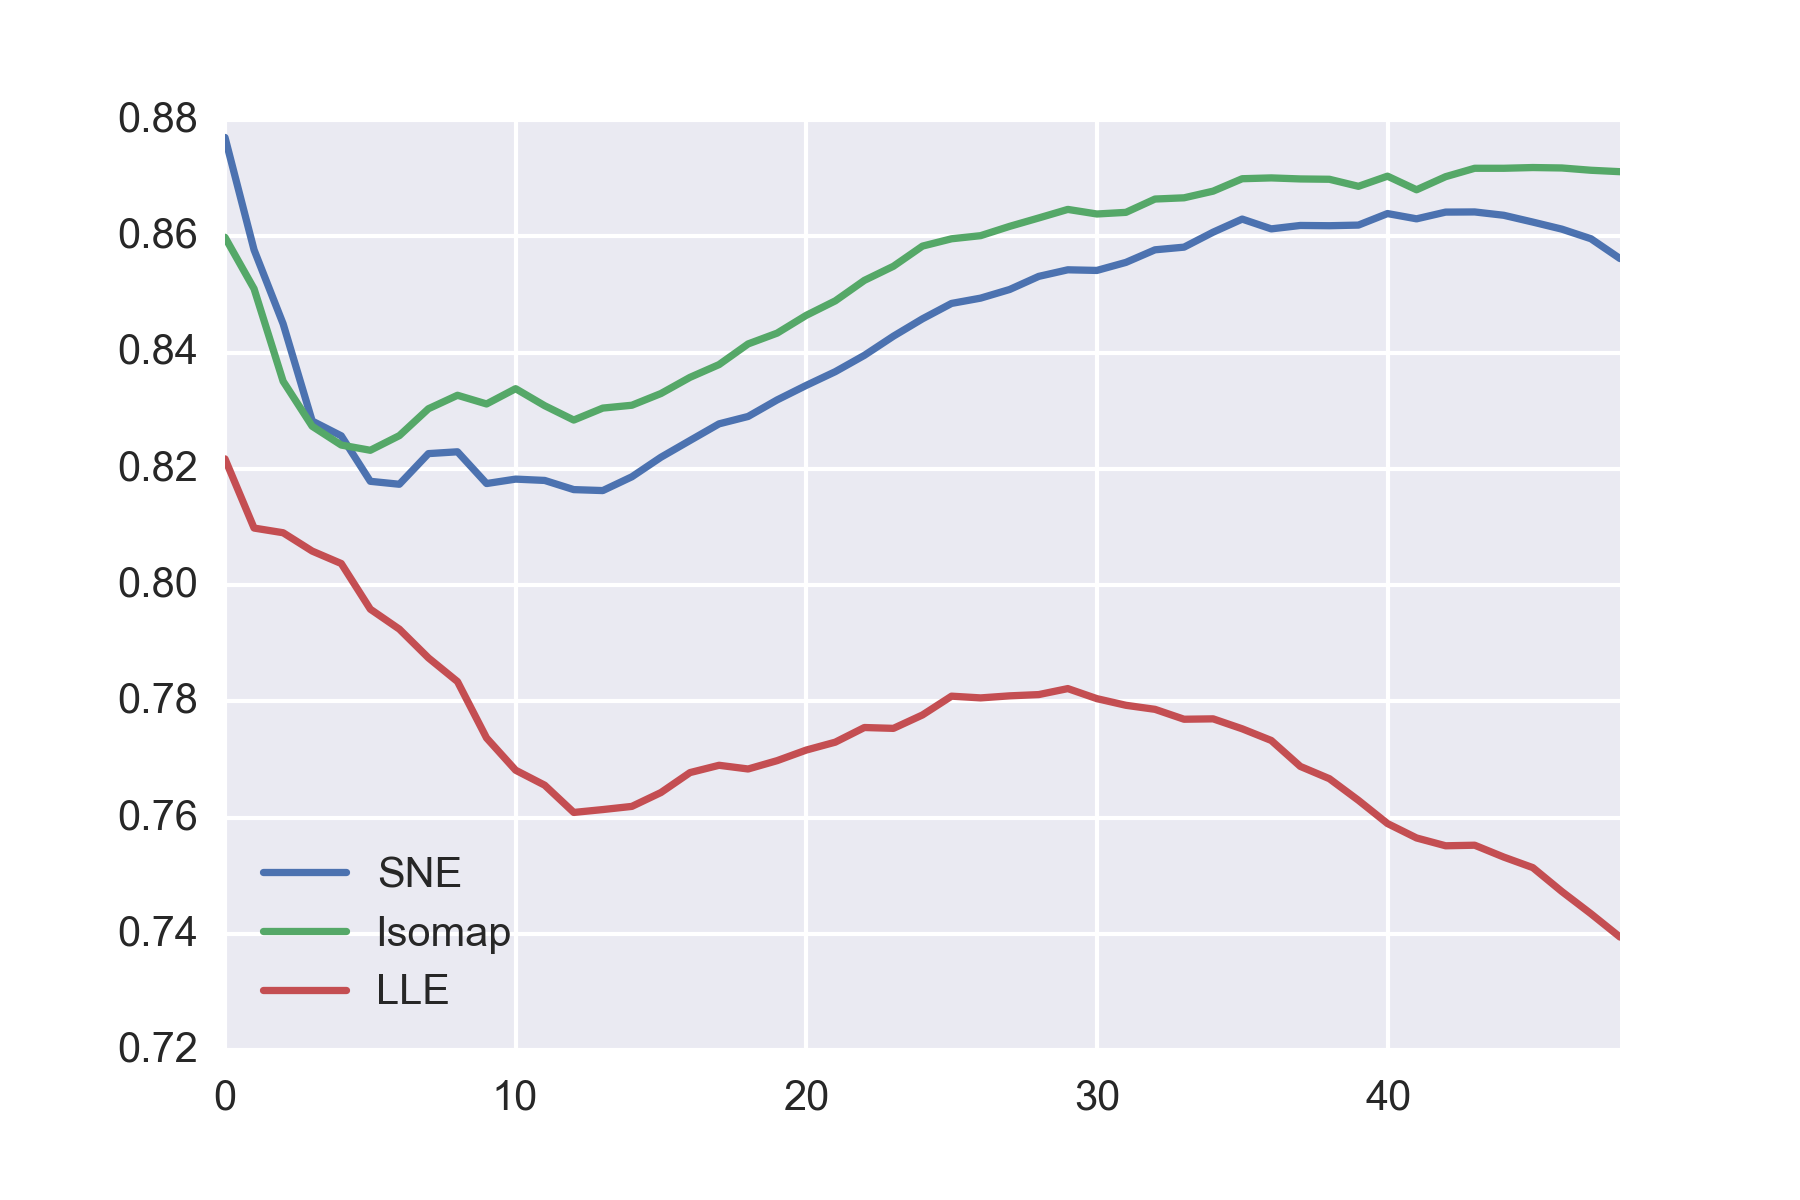
\includegraphics[width=0.49\textwidth]{figures/quality_measures/line_continuity_2d.png}}
	\caption{Trustworthiness and continuity of the 2D projections produced from line features.}\label{fig:TC_2d_blobs}
\end{figure}

\begin{figure}[H]
	\centering
	\subfigure{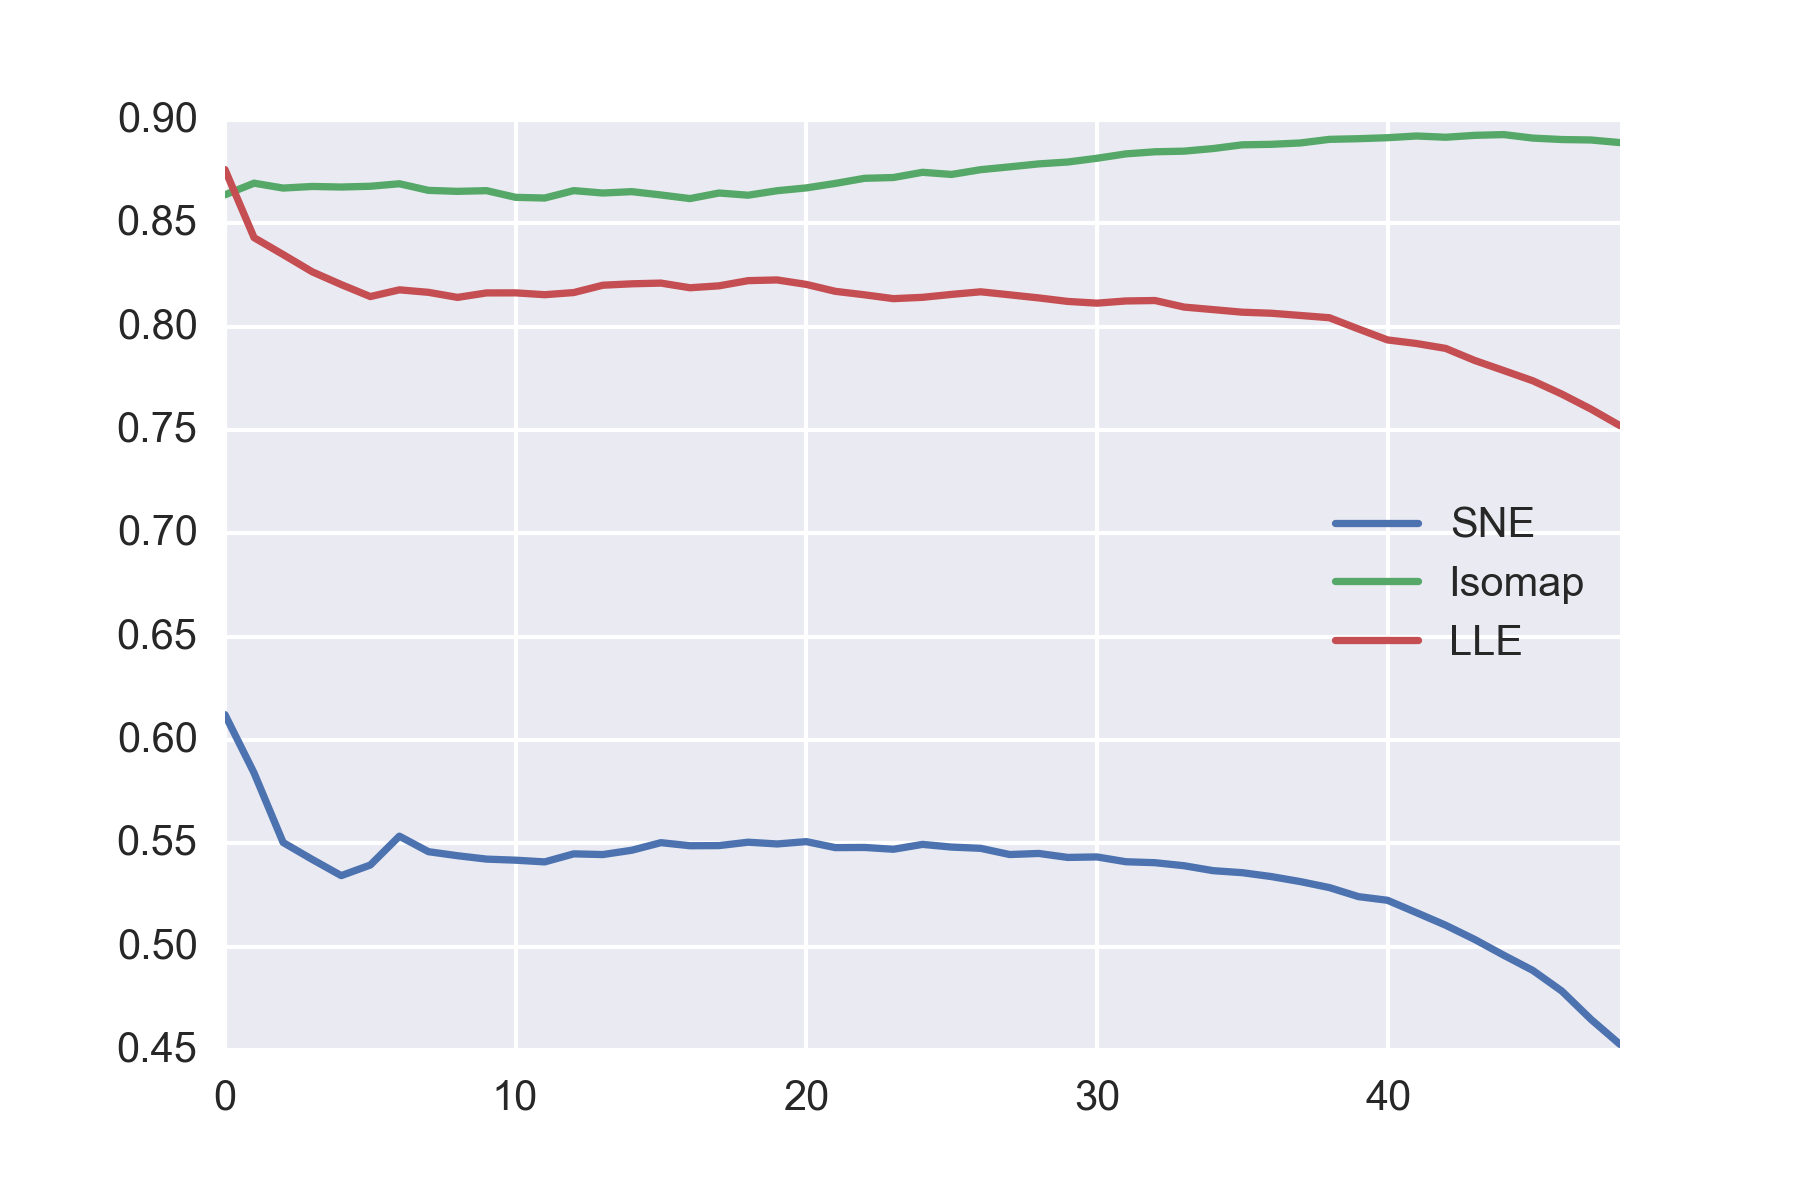
\includegraphics[width=0.49\textwidth]{figures/quality_measures/line_trustworthiness_3d.png}}
	\subfigure{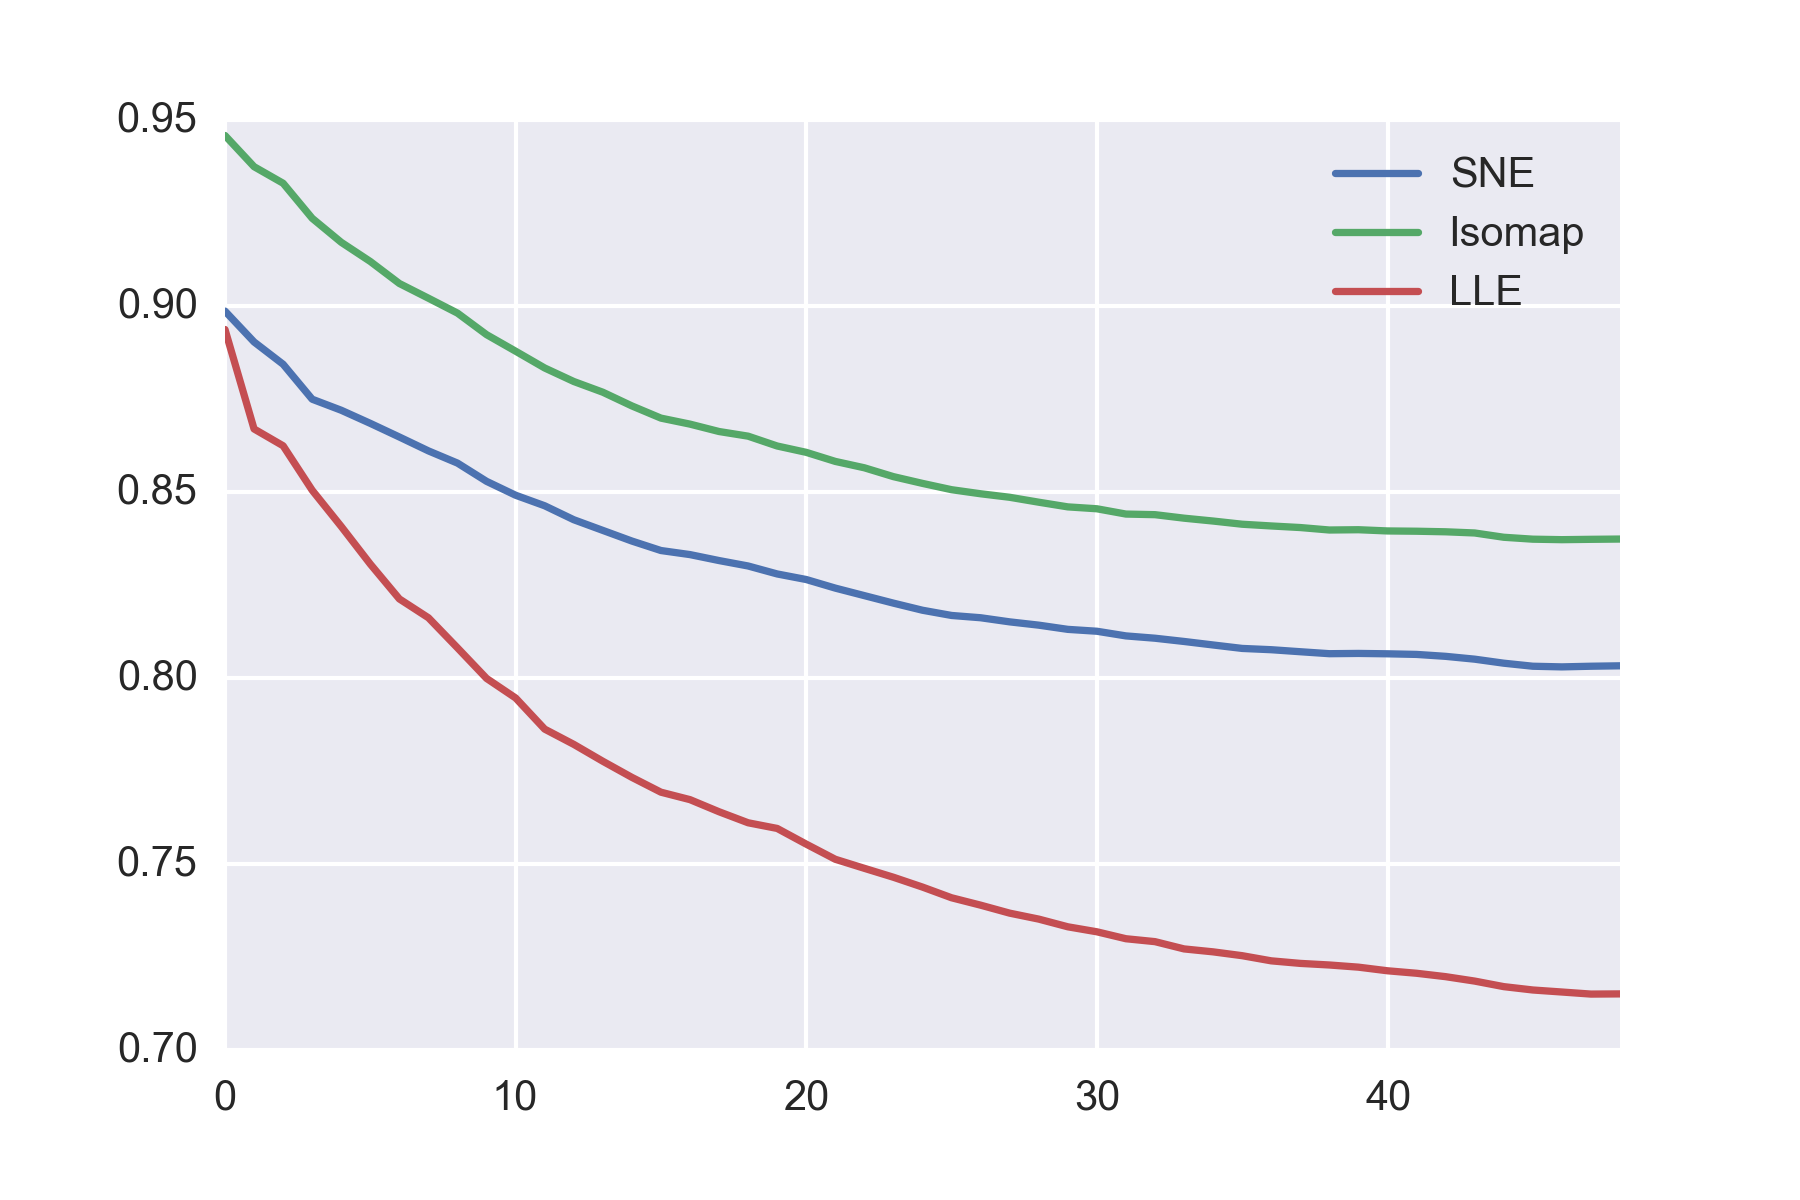
\includegraphics[width=0.49\textwidth]{figures/quality_measures/line_continuity_3d.png}}
	\caption{Trustworthiness and continuity of the 3D projections produced from line features.}\label{fig:TC_3d_blobs}
\end{figure}

\begin{figure}[H]
	\centering
	\subfigure{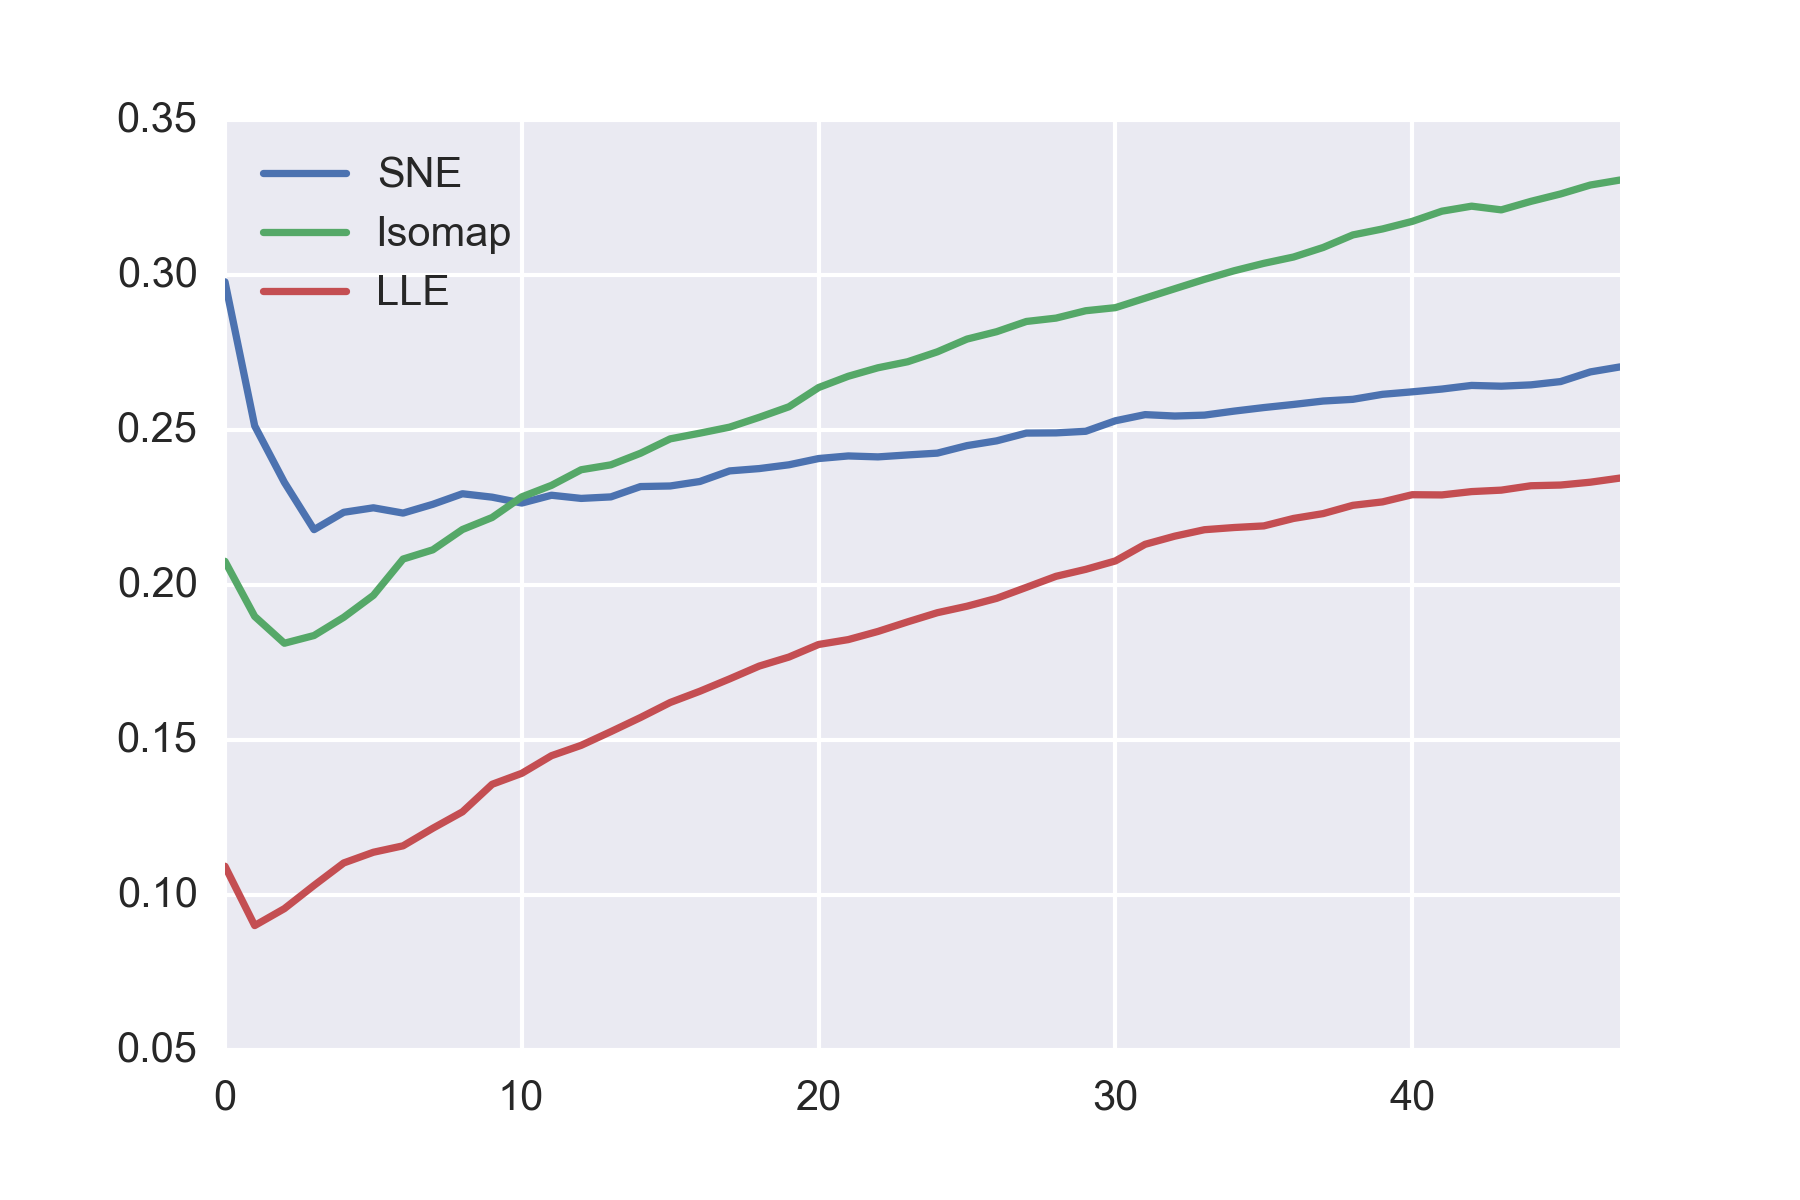
\includegraphics[width=0.49\textwidth]{figures/quality_measures/line_lcmc_2d.png}}
	\subfigure{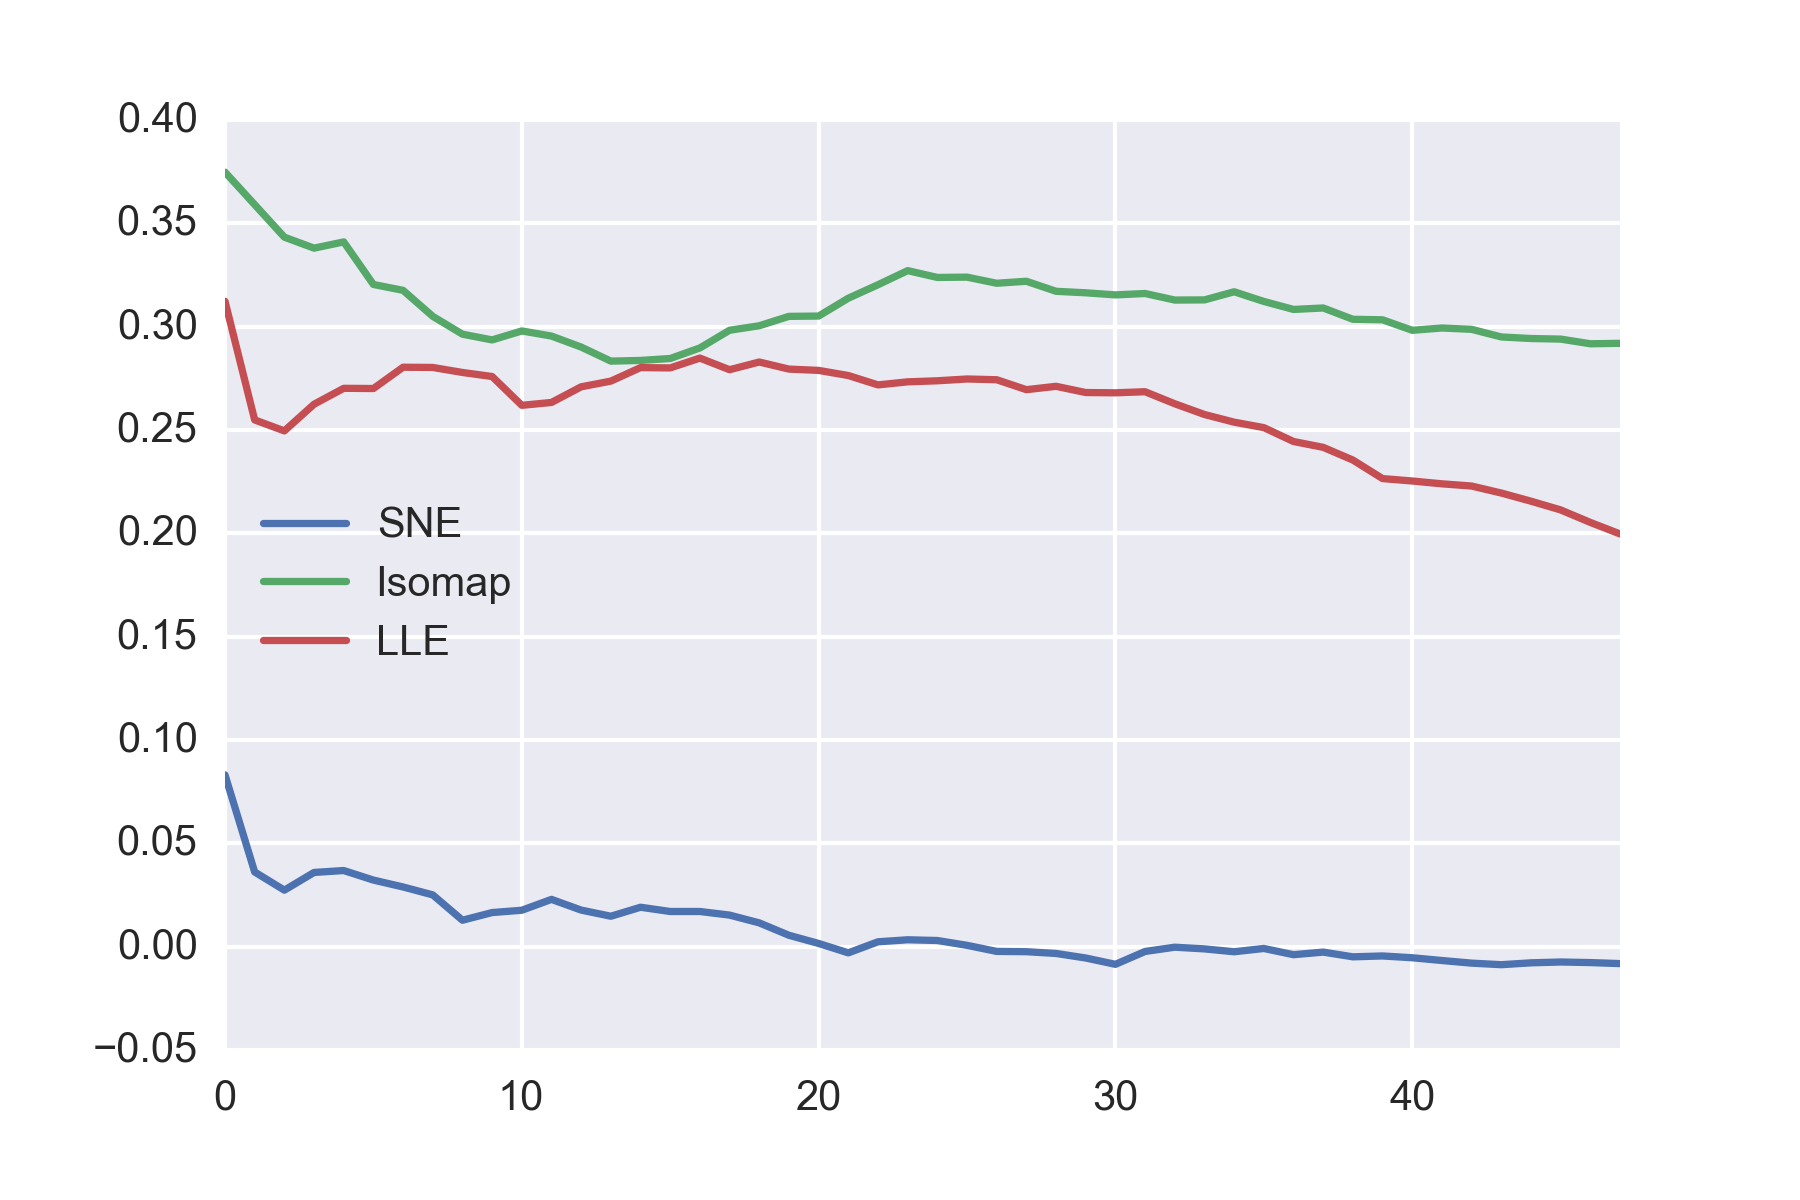
\includegraphics[width=0.49\textwidth]{figures/quality_measures/line_lcmc_3d.png}}
	\caption{LCMC of both the 2D projection (left) and 3D projection (right) of the feature space for lines.}\label{fig:LCMC_blobs}
\end{figure}

\clearpage

\clearpage
\begin{figure}[H]
	\centering
	\subfigure{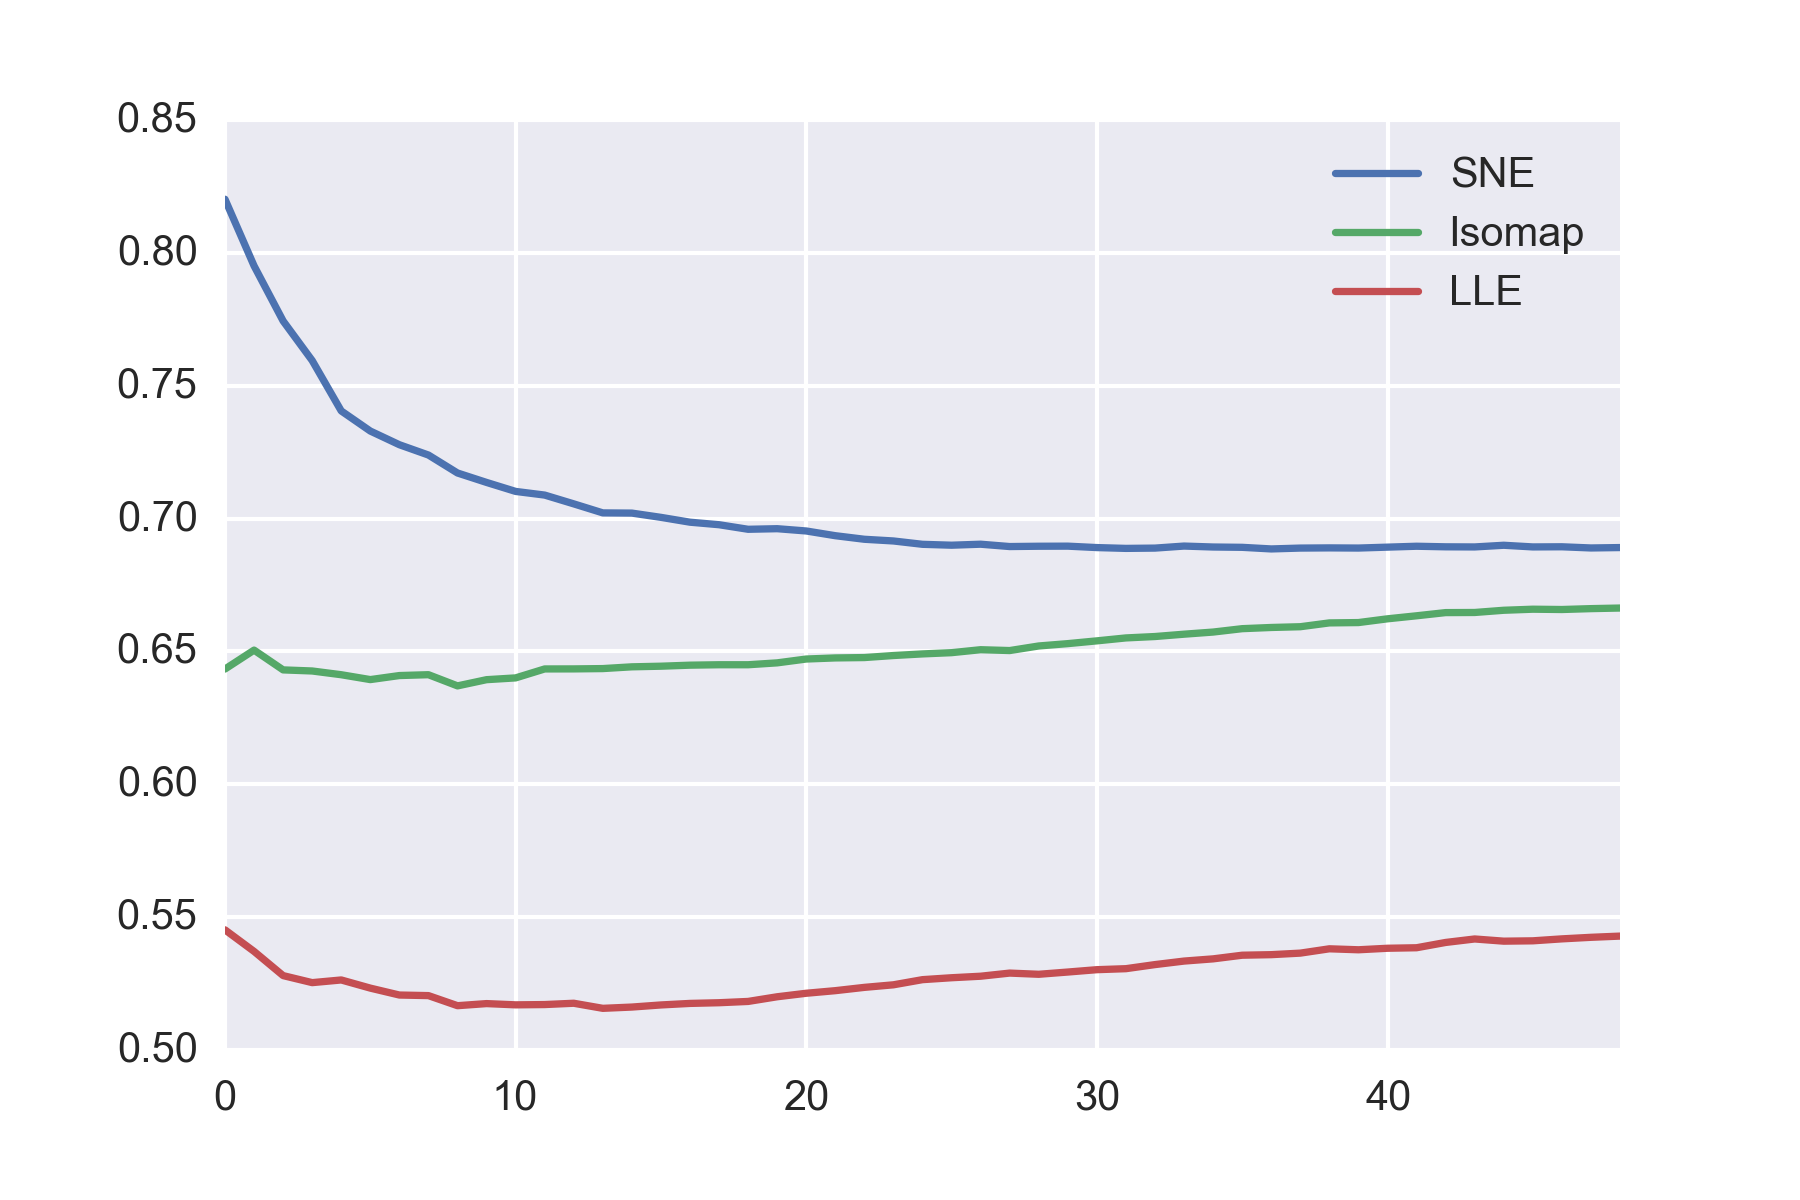
\includegraphics[width=0.49\textwidth]{figures/quality_measures/intensity_trustworthiness_2d.png}}
	\subfigure{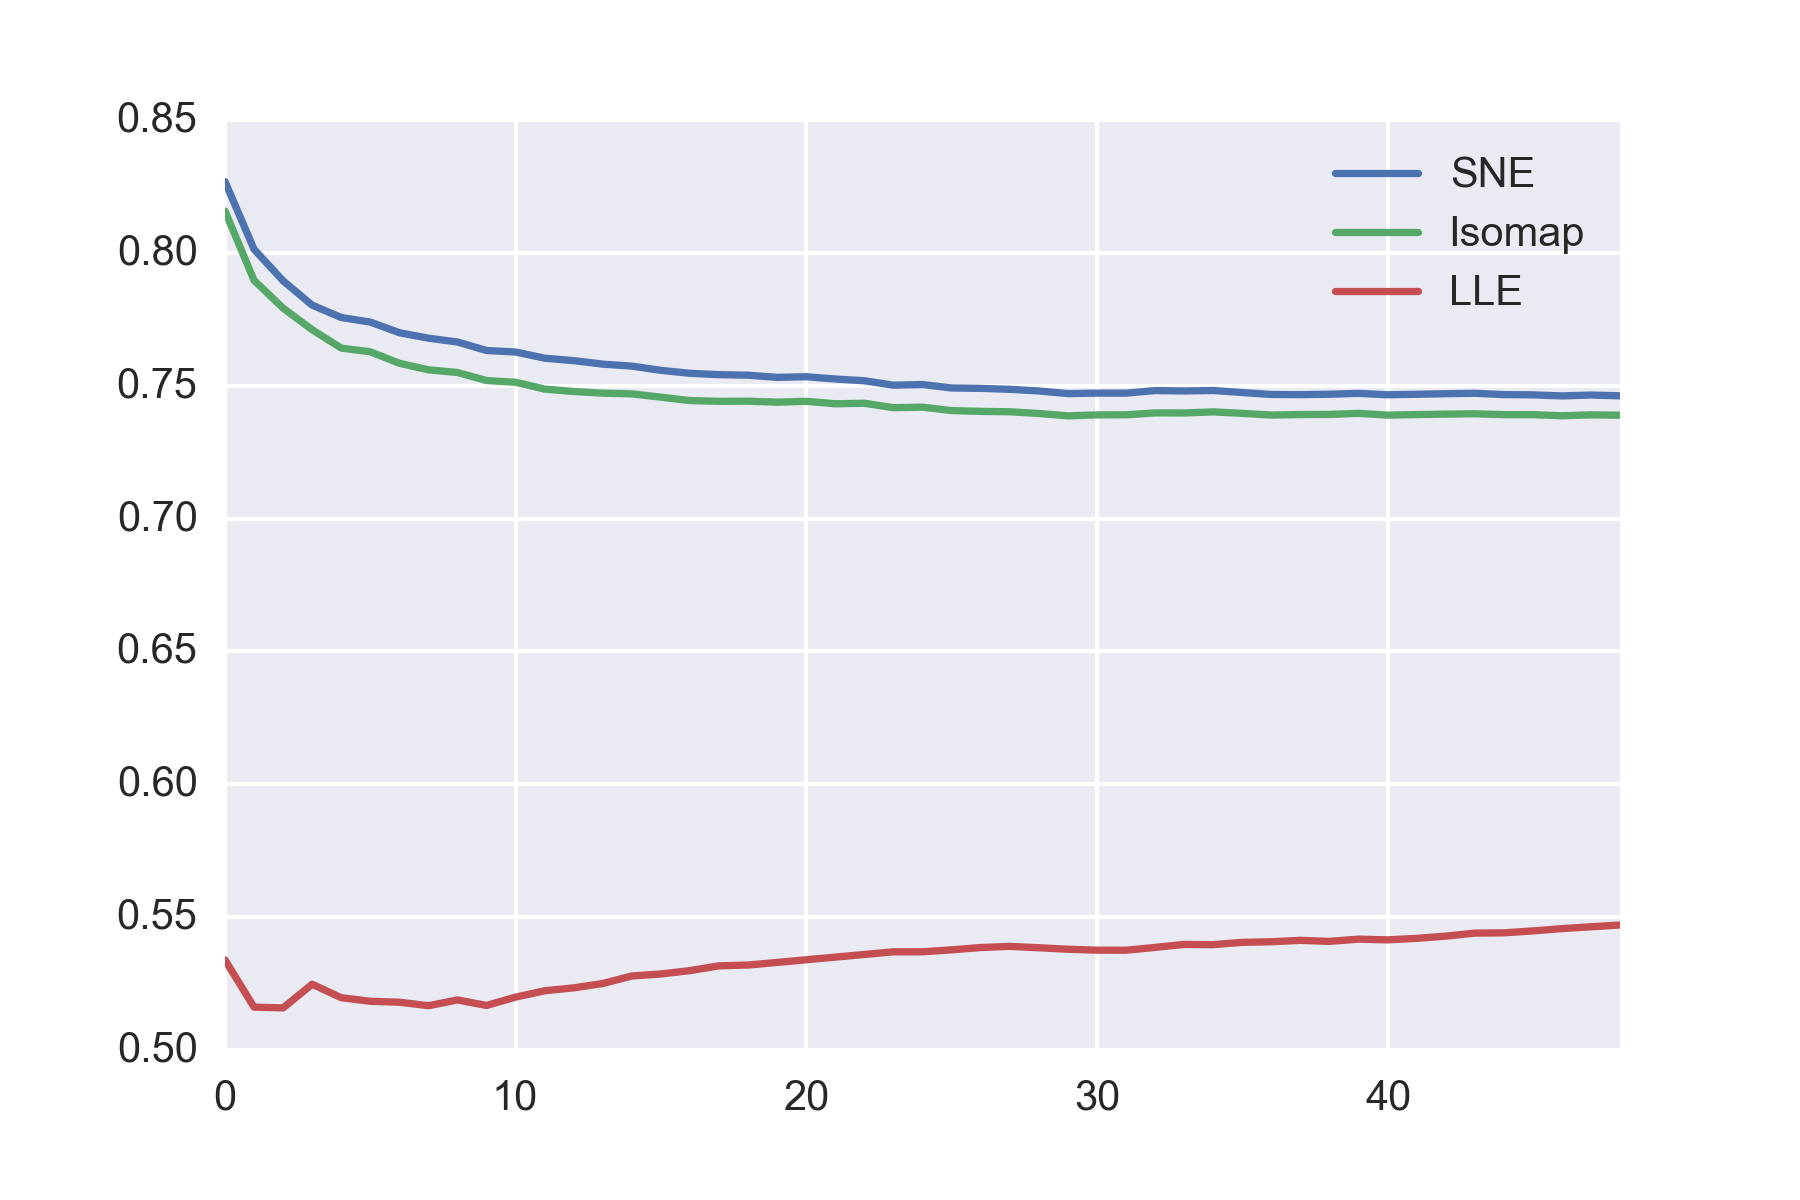
\includegraphics[width=0.49\textwidth]{figures/quality_measures/intensity_continuity_2d.png}}
	\caption{Trustworthiness and continuity of the 2D projections produced from intensity features from blobs.}\label{fig:TC_2d_blobs}
\end{figure}

\begin{figure}[H]
	\centering
	\subfigure{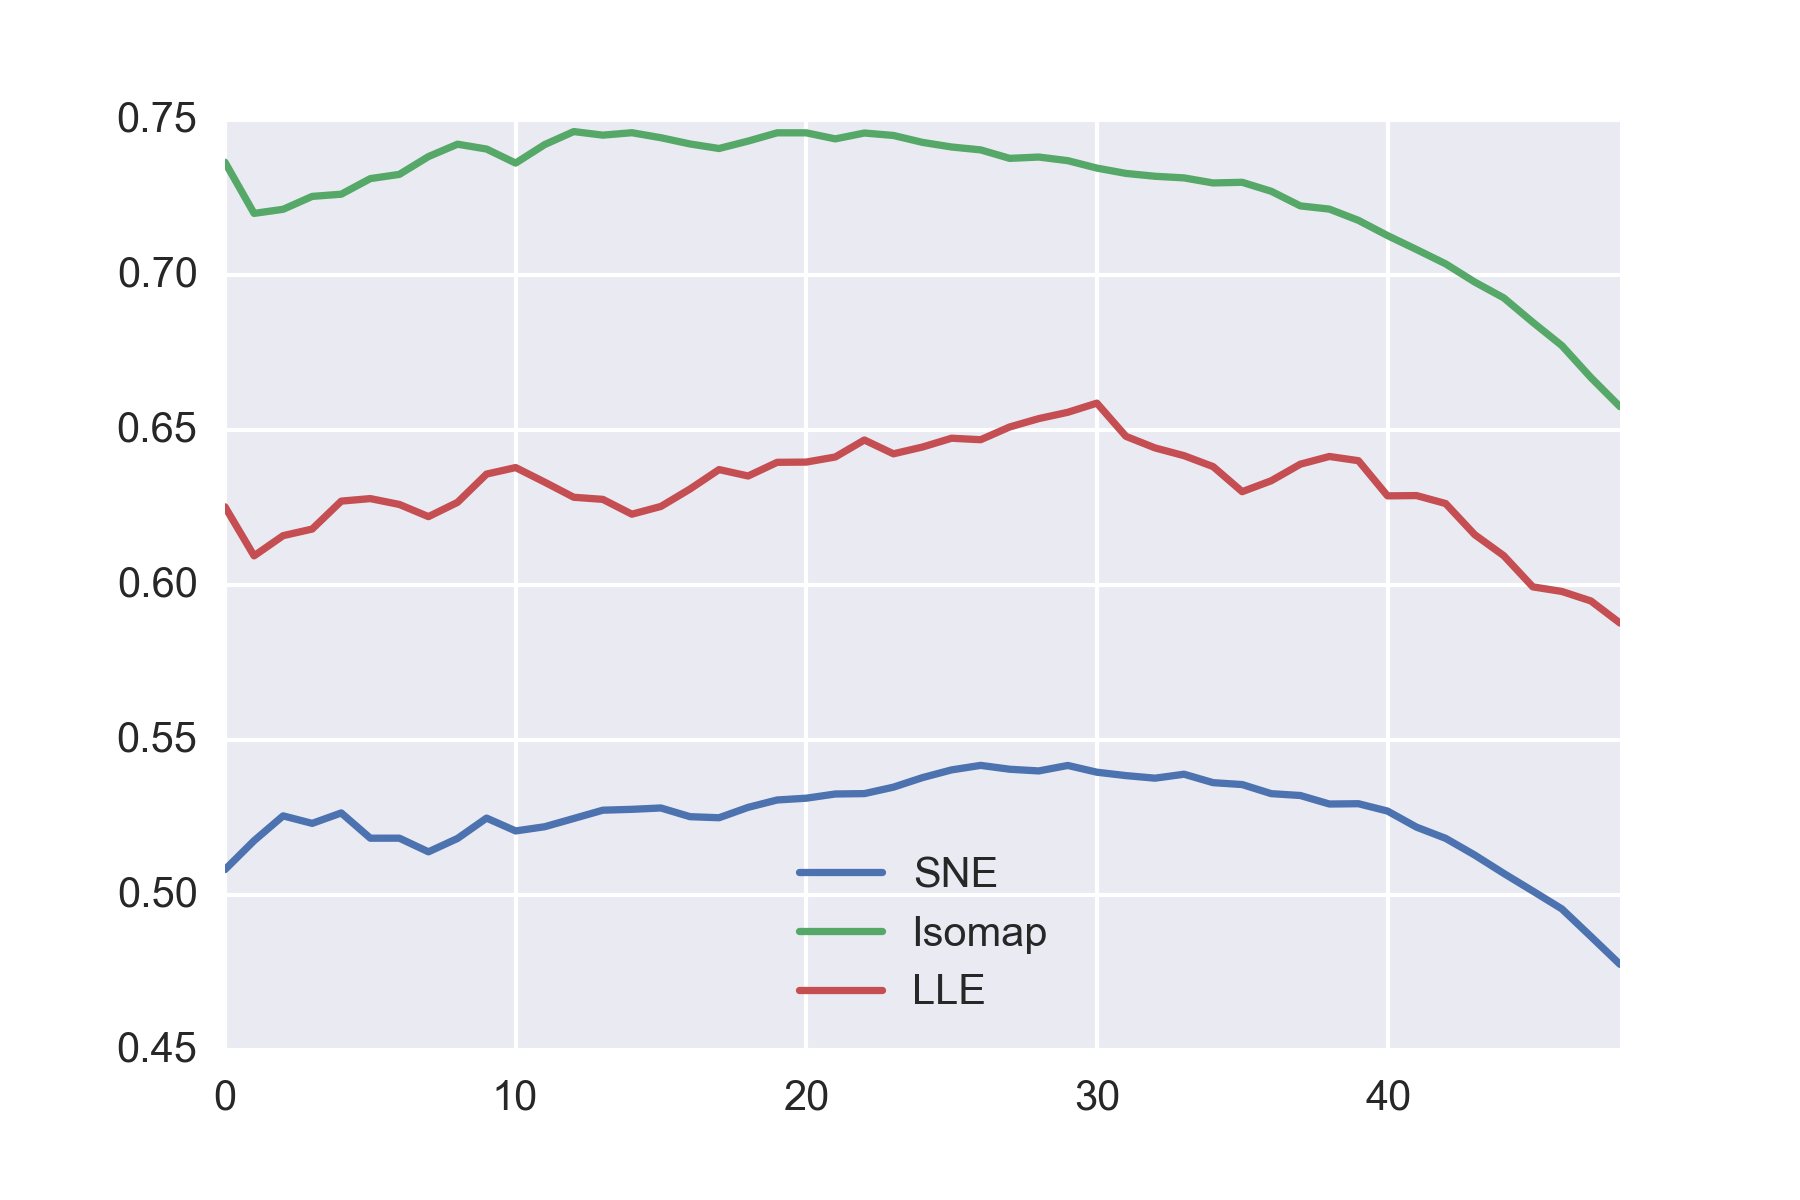
\includegraphics[width=0.49\textwidth]{figures/quality_measures/intensity_trustworthiness_3d.png}}
	\subfigure{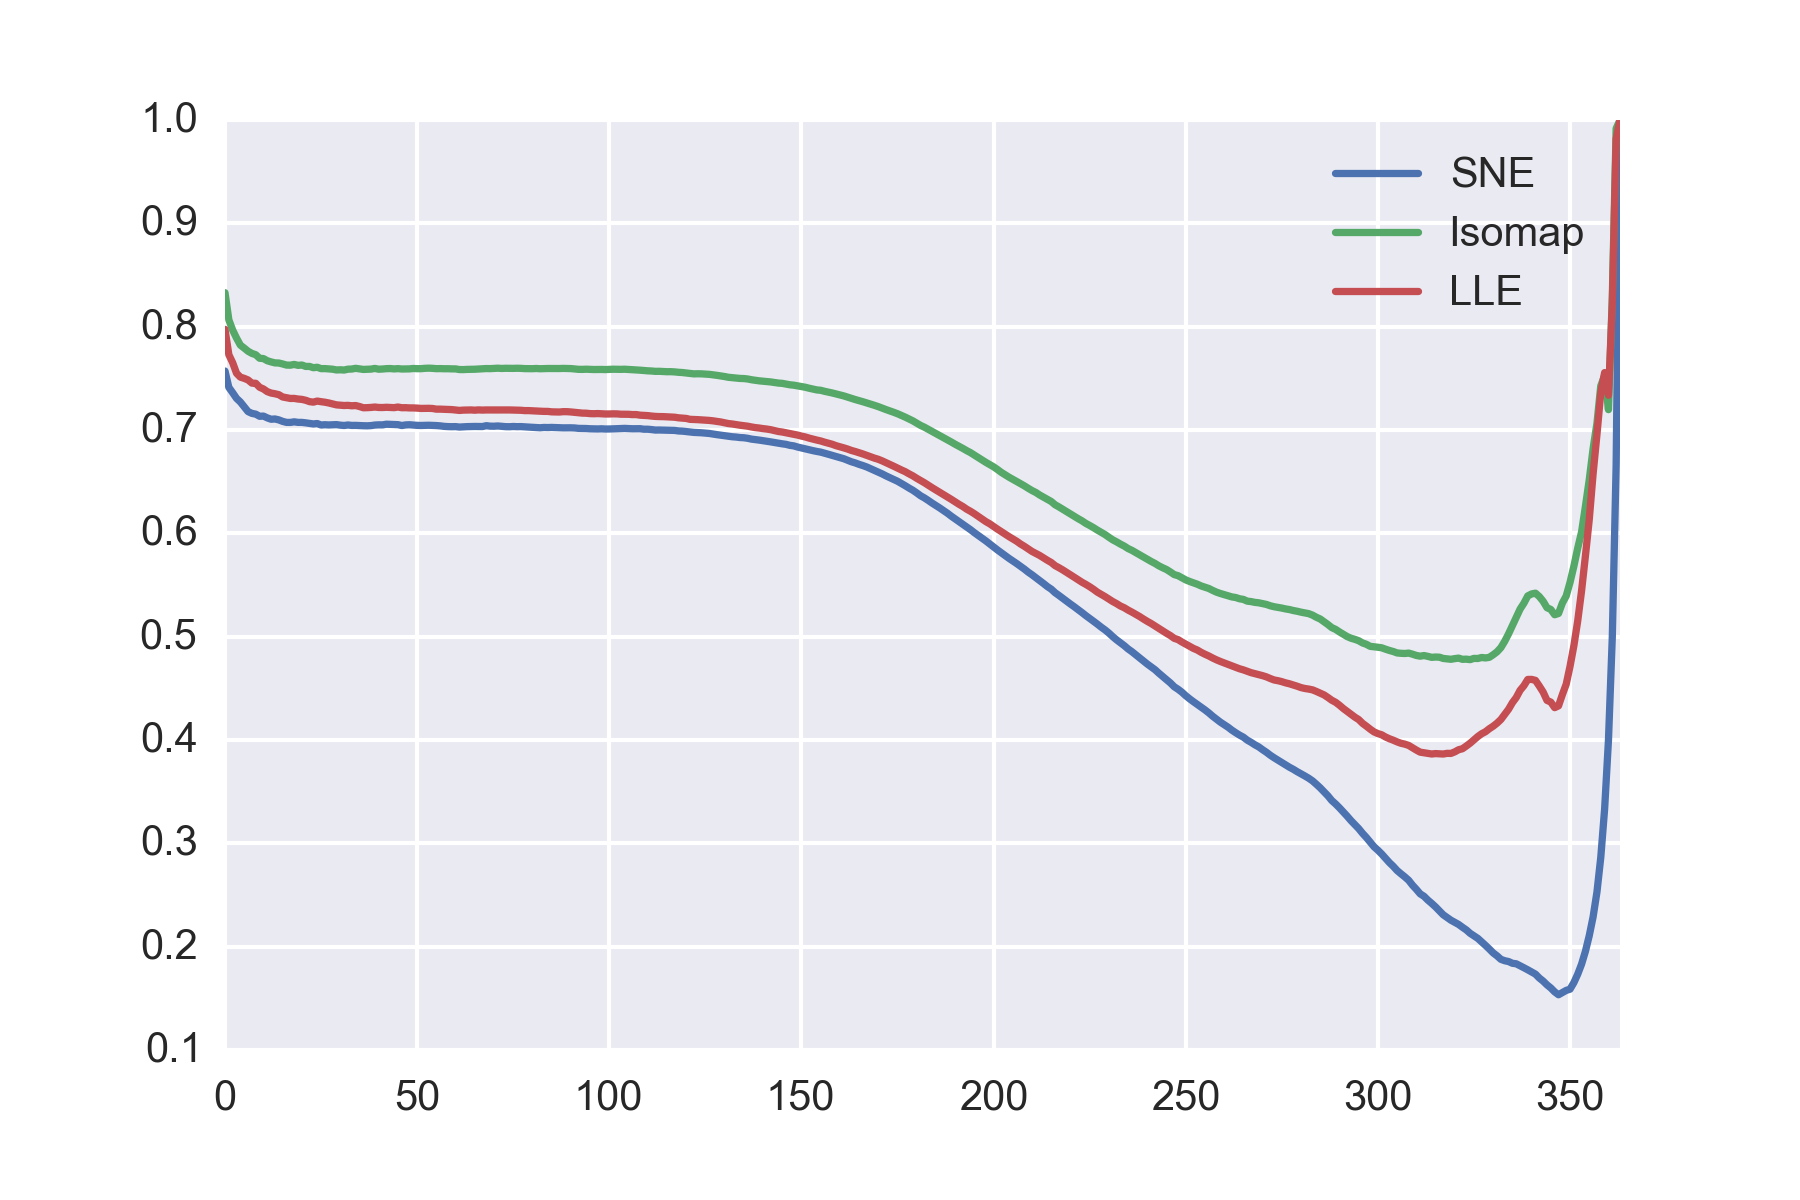
\includegraphics[width=0.49\textwidth]{figures/quality_measures/intensity_continuity_3d.png}}
	\caption{Trustworthiness and continuity of the 3D projections produced from intensity features from blobs.}\label{fig:TC_3d_blobs}
\end{figure}

\begin{figure}[H]
	\centering
	\subfigure{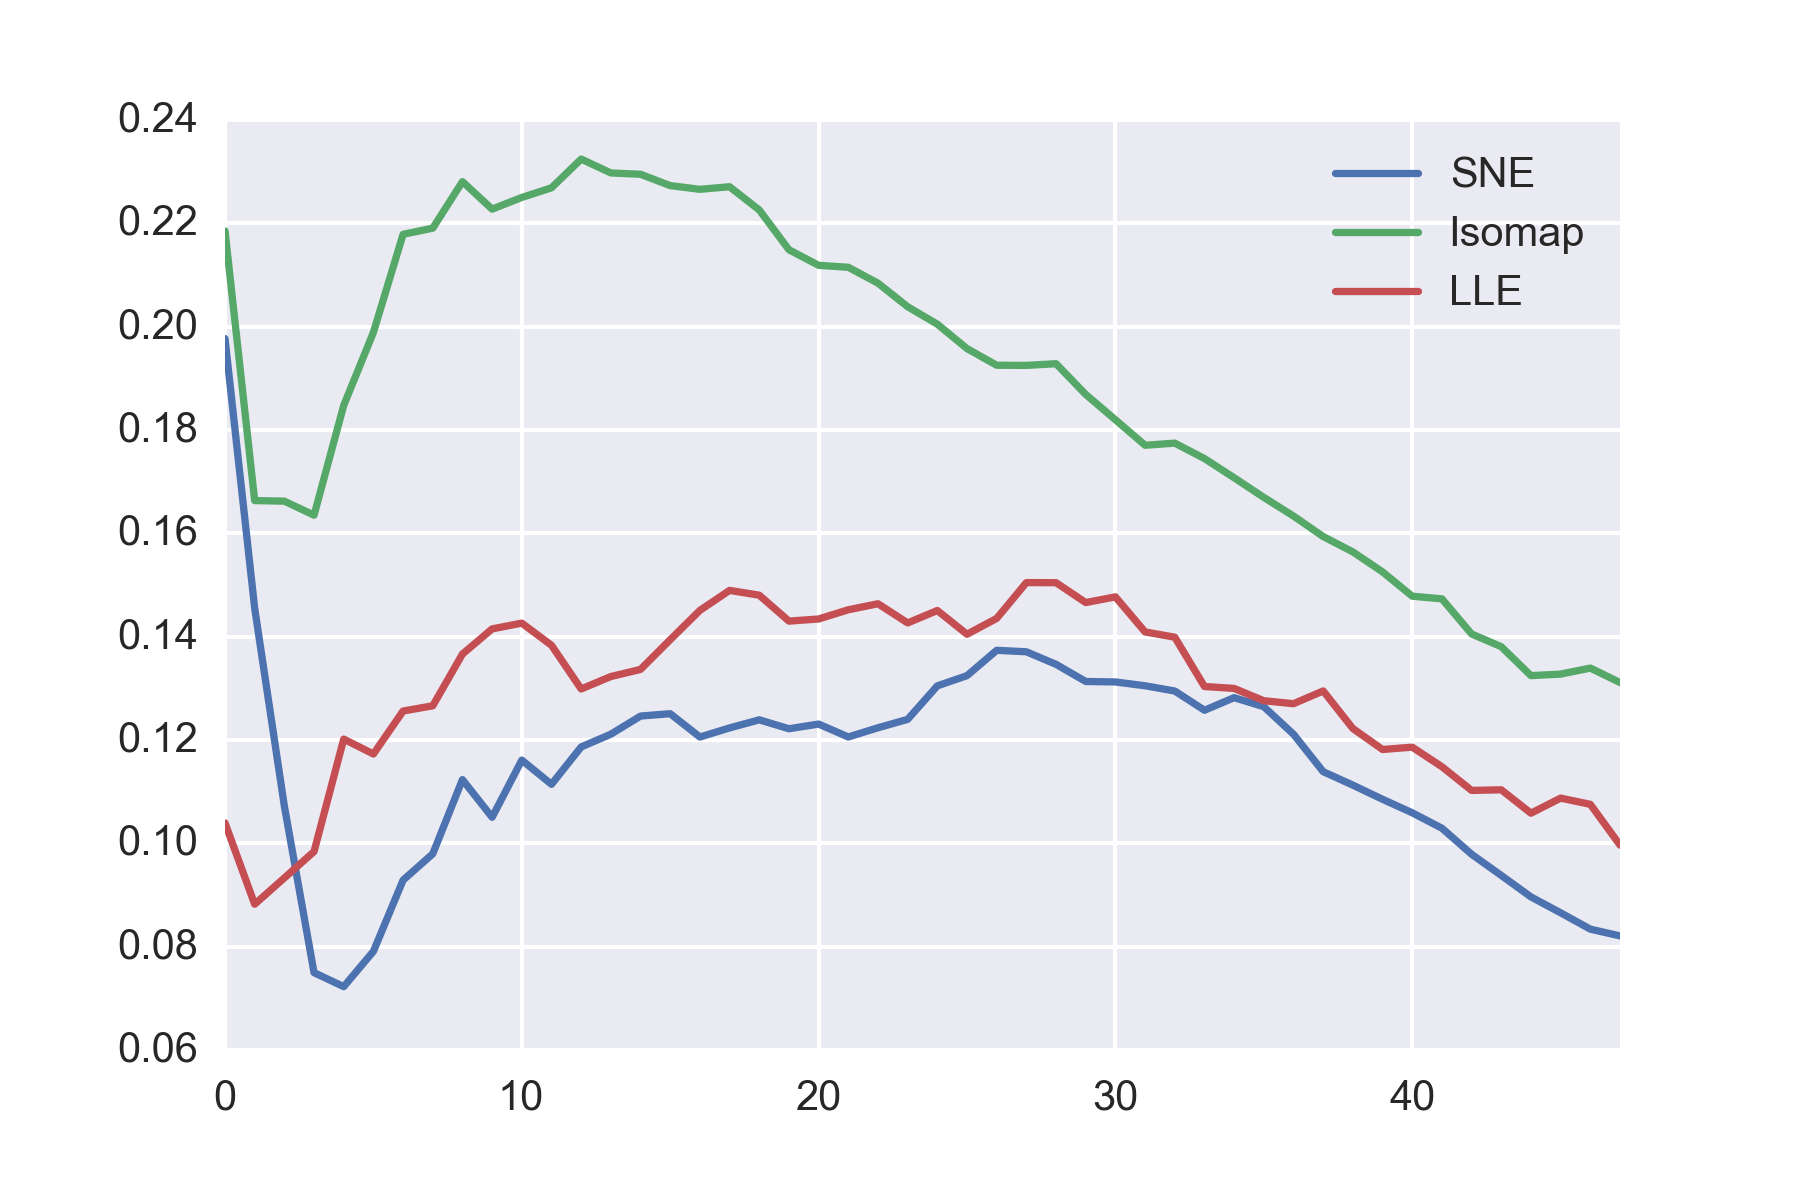
\includegraphics[width=0.49\textwidth]{figures/quality_measures/intensity_lcmc_2d.png}}
	\subfigure{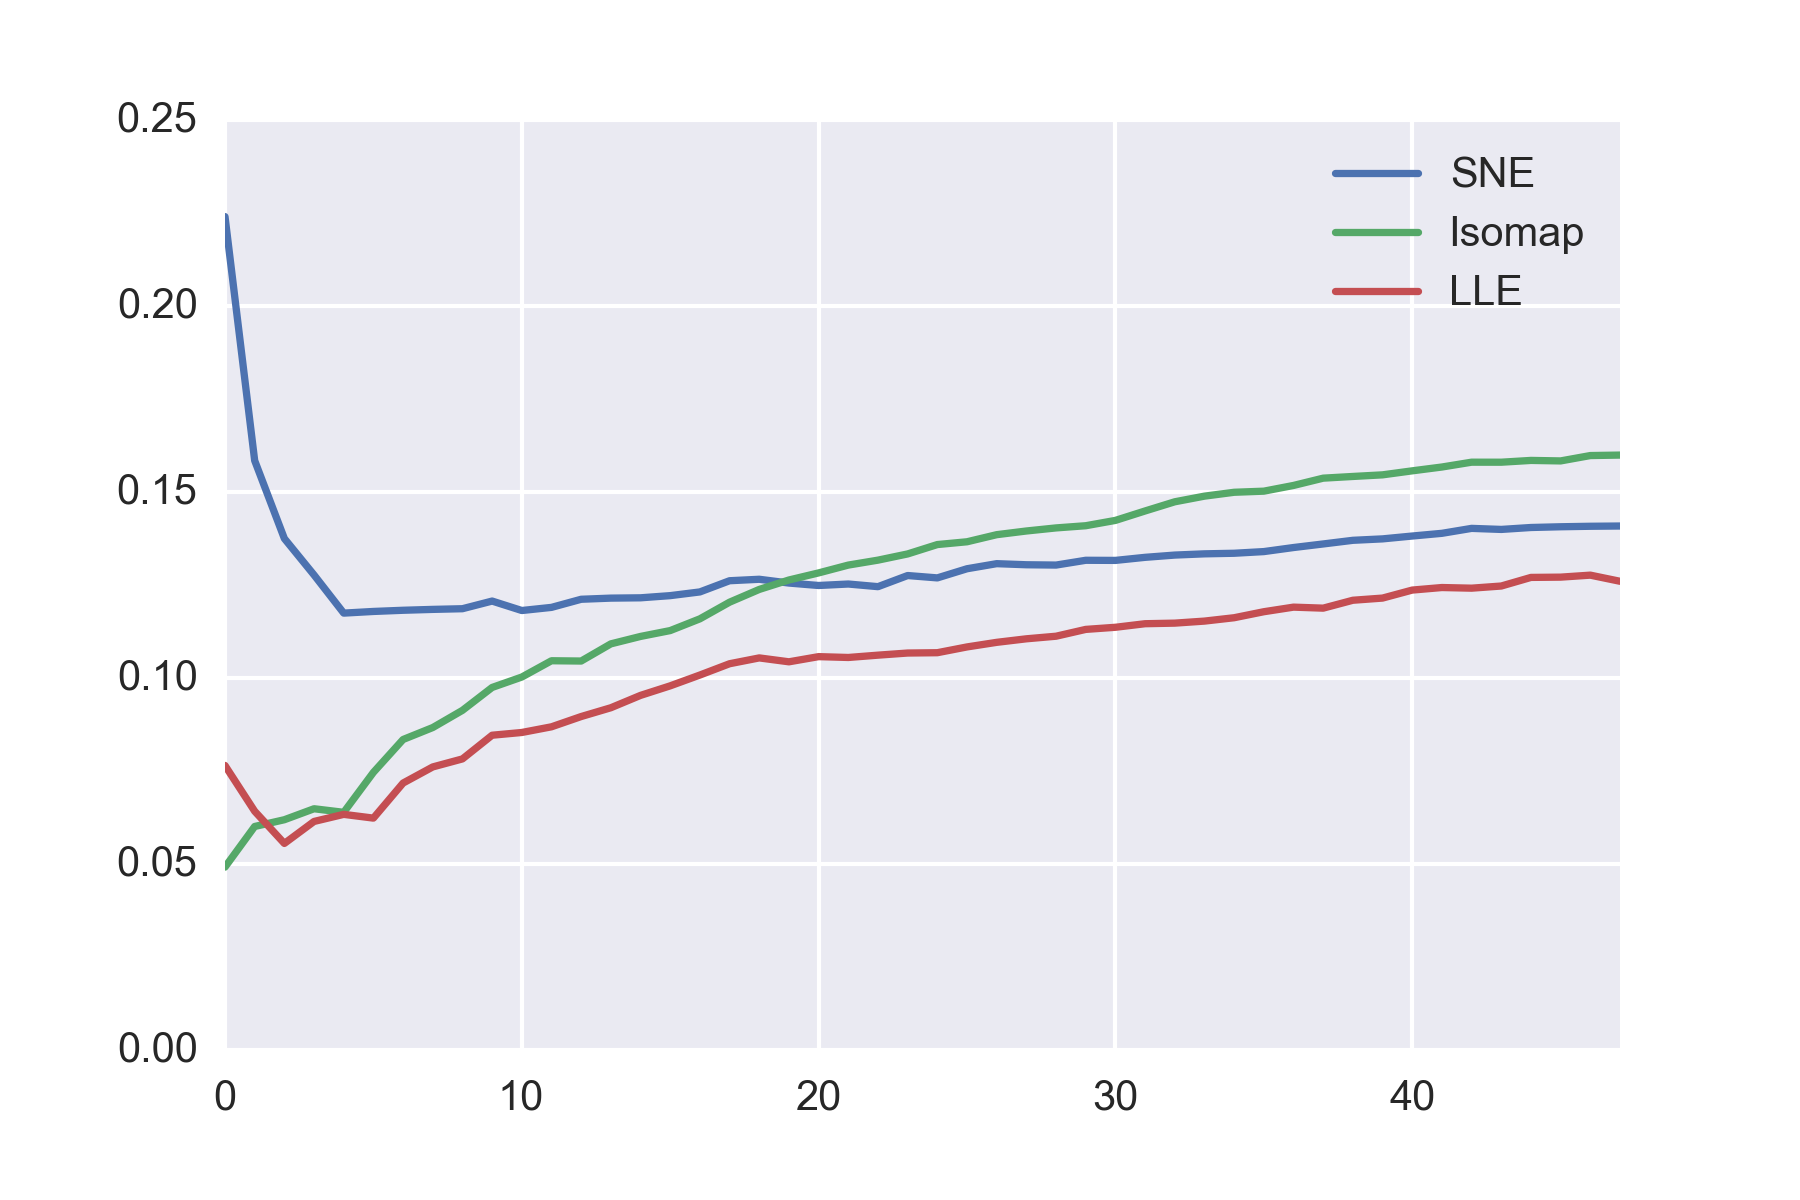
\includegraphics[width=0.49\textwidth]{figures/quality_measures/intensity_lcmc_3d.png}}
	\caption{LCMC of both the 2D projection (left) and 3D projection (right) of the feature space for intensity from blobs.}\label{fig:LCMC_blobs}
\end{figure}
\clearpage

\clearpage
\begin{figure}[H]
	\centering
	\subfigure{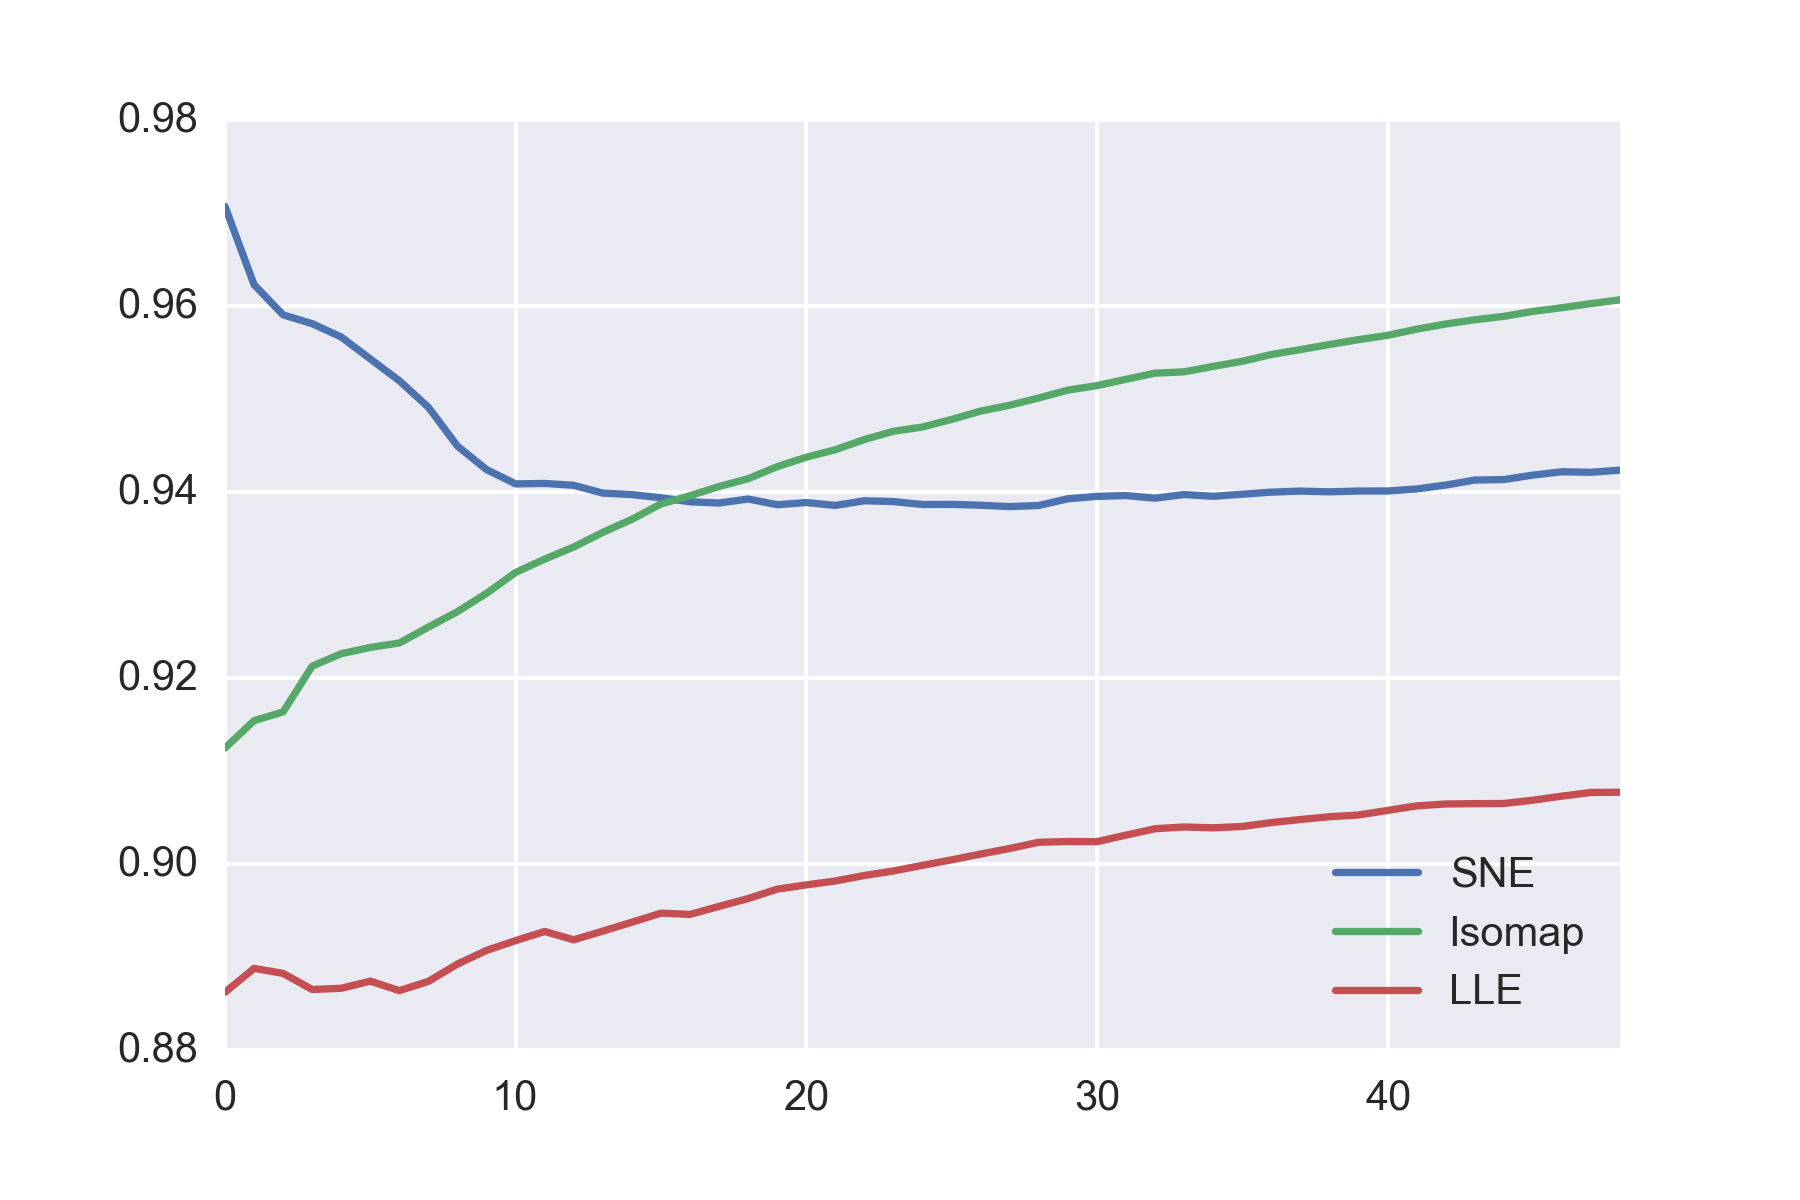
\includegraphics[width=0.49\textwidth]{figures/quality_measures/texture_trustworthiness_2d.png}}
	\subfigure{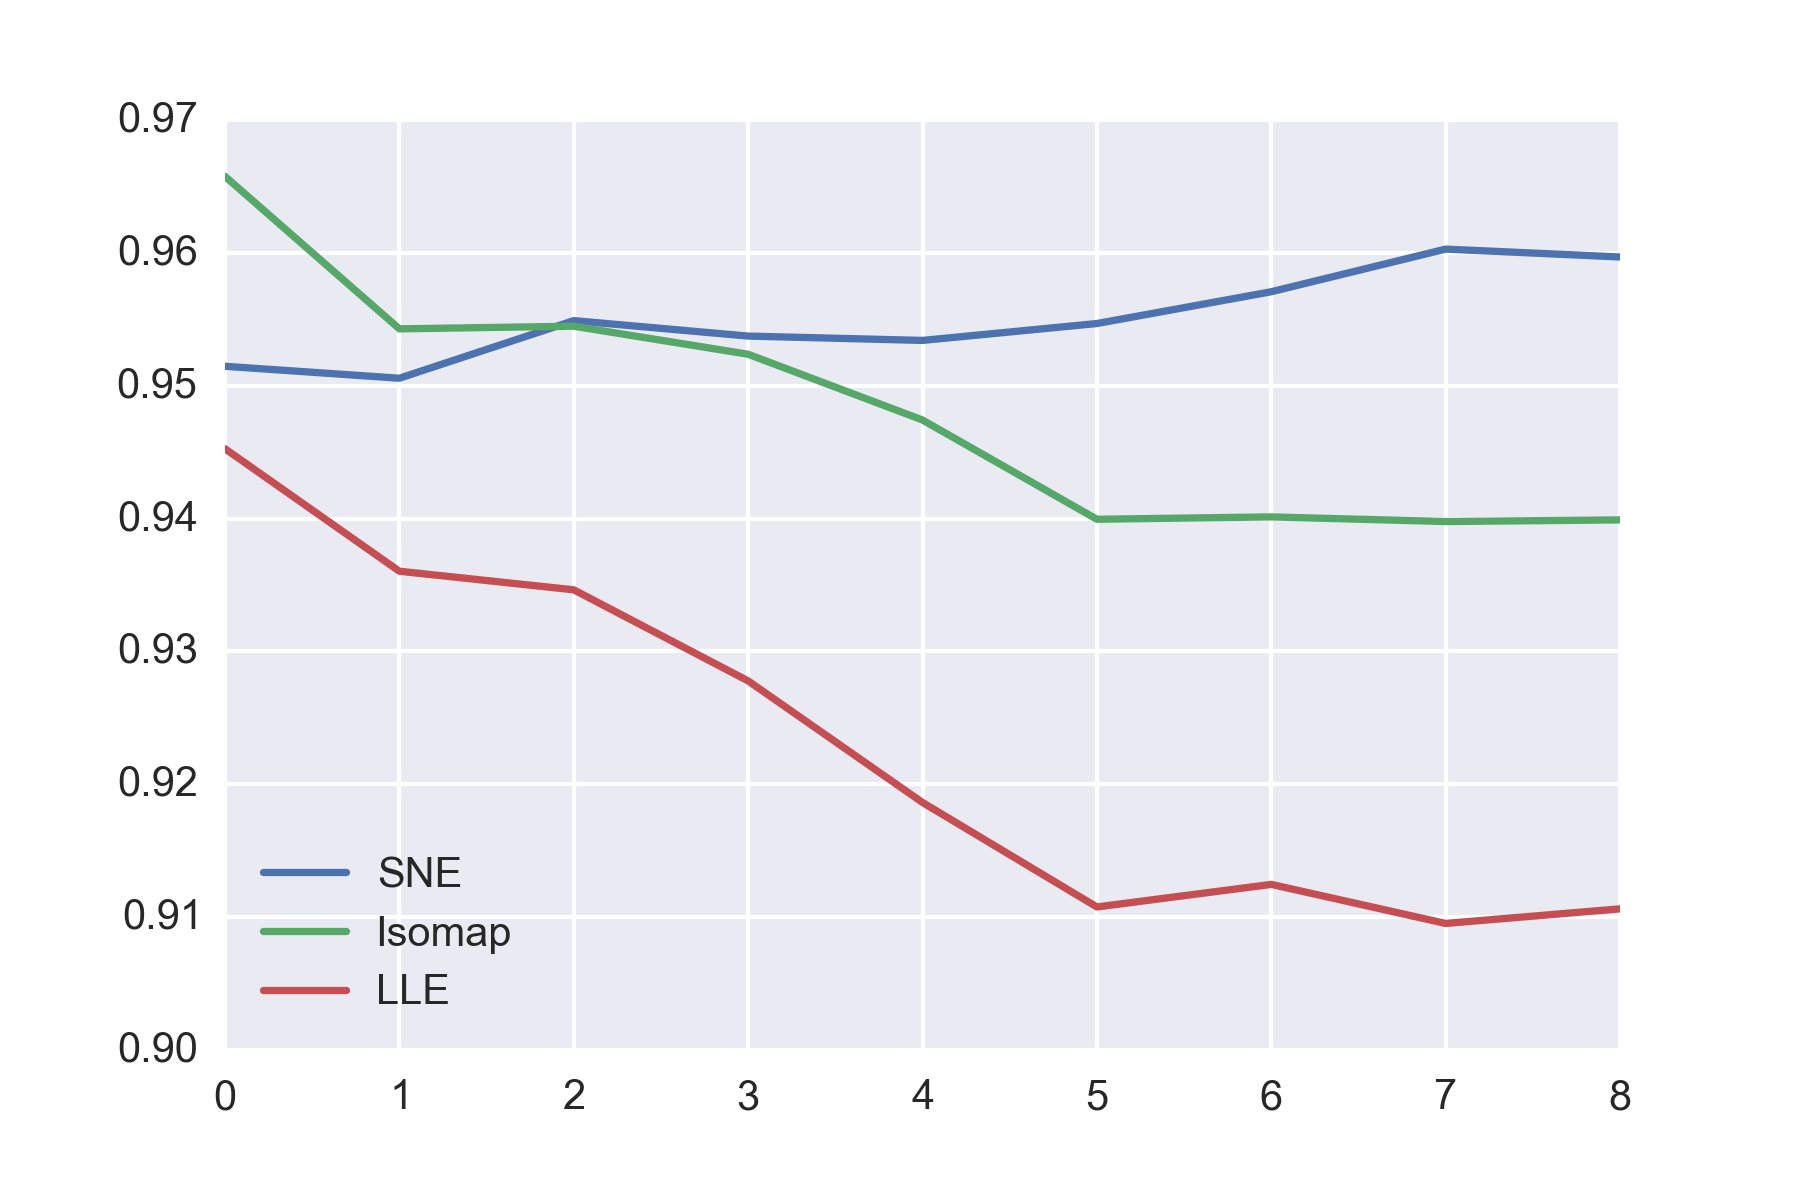
\includegraphics[width=0.49\textwidth]{figures/quality_measures/texture_continuity_2d.png}}
	\caption{Trustworthiness and continuity of the 2D projections produced from texture features from blobs.}\label{fig:TC_2d_blobs}
\end{figure}

\begin{figure}[H]
	\centering
	\subfigure{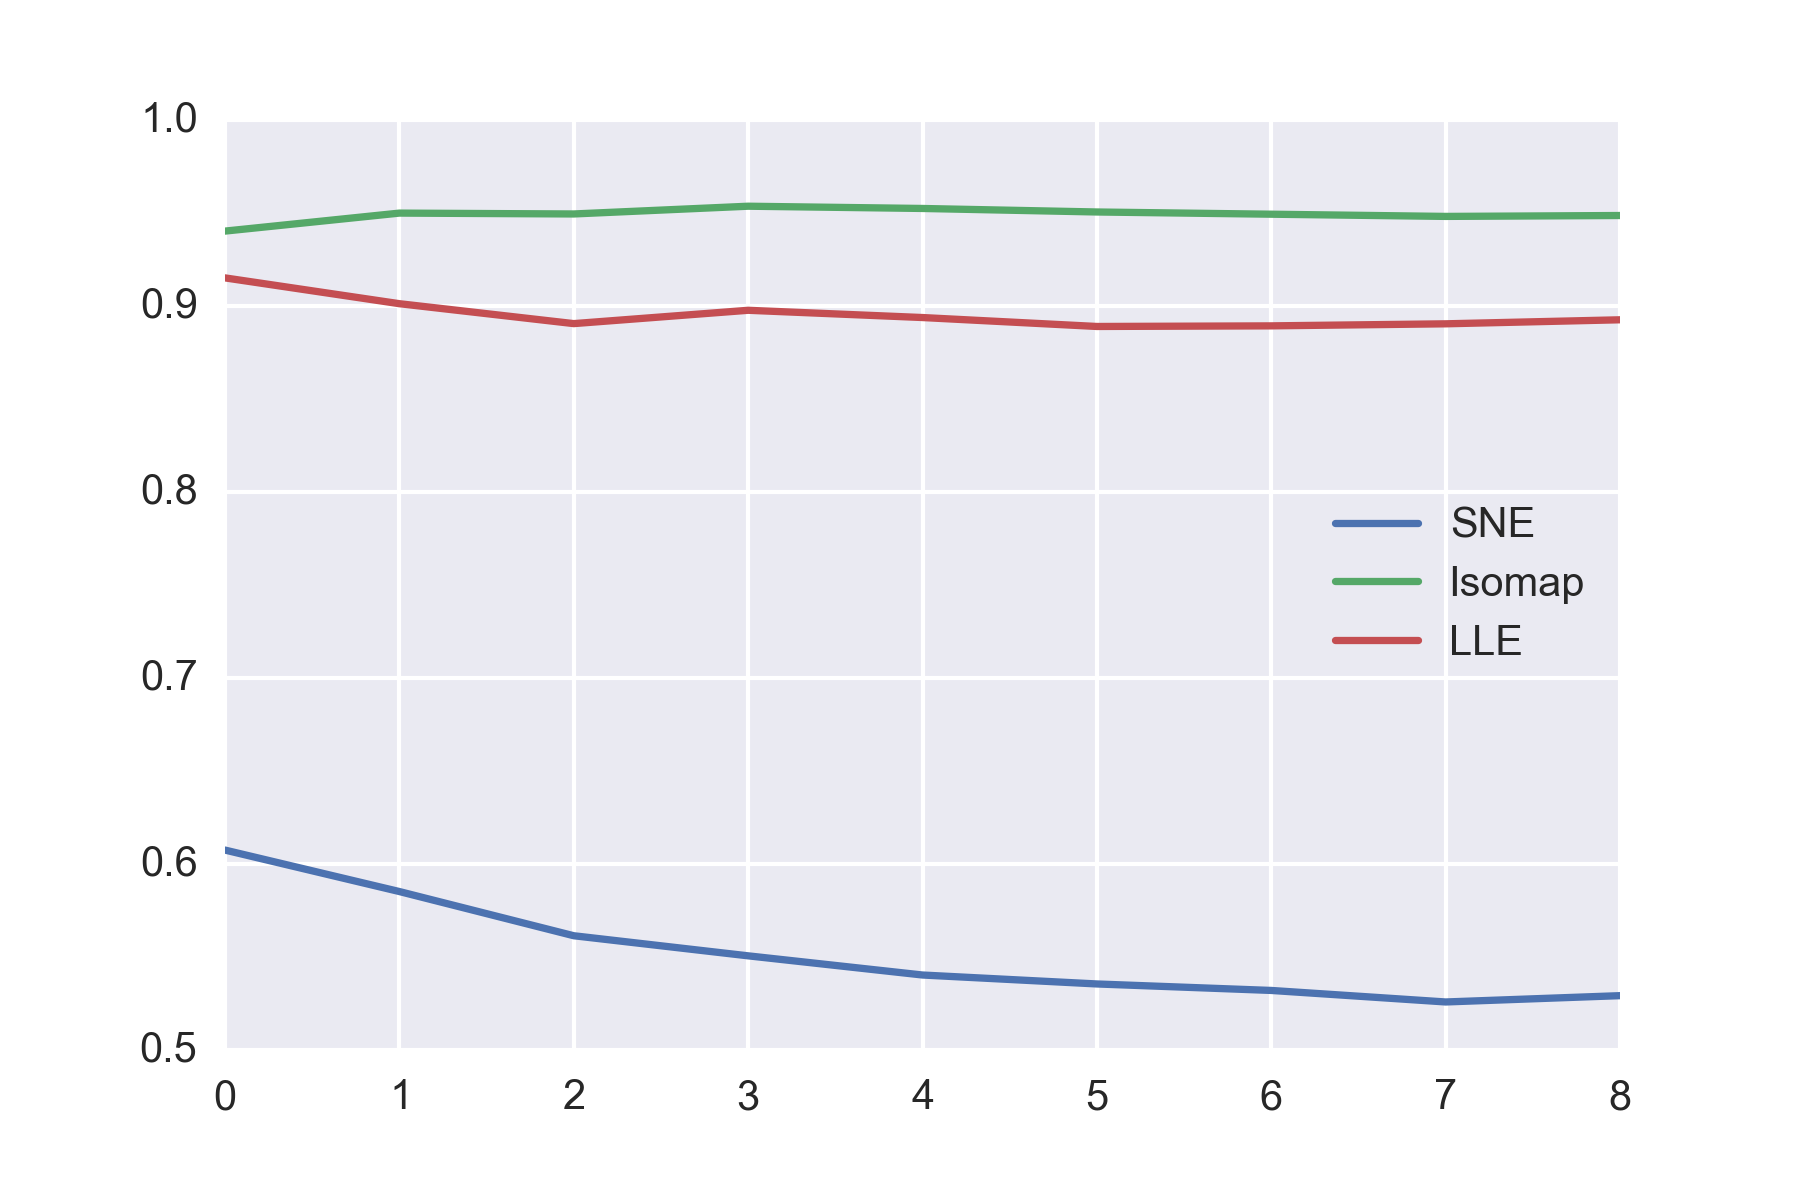
\includegraphics[width=0.49\textwidth]{figures/quality_measures/texture_trustworthiness_3d.png}}
	\subfigure{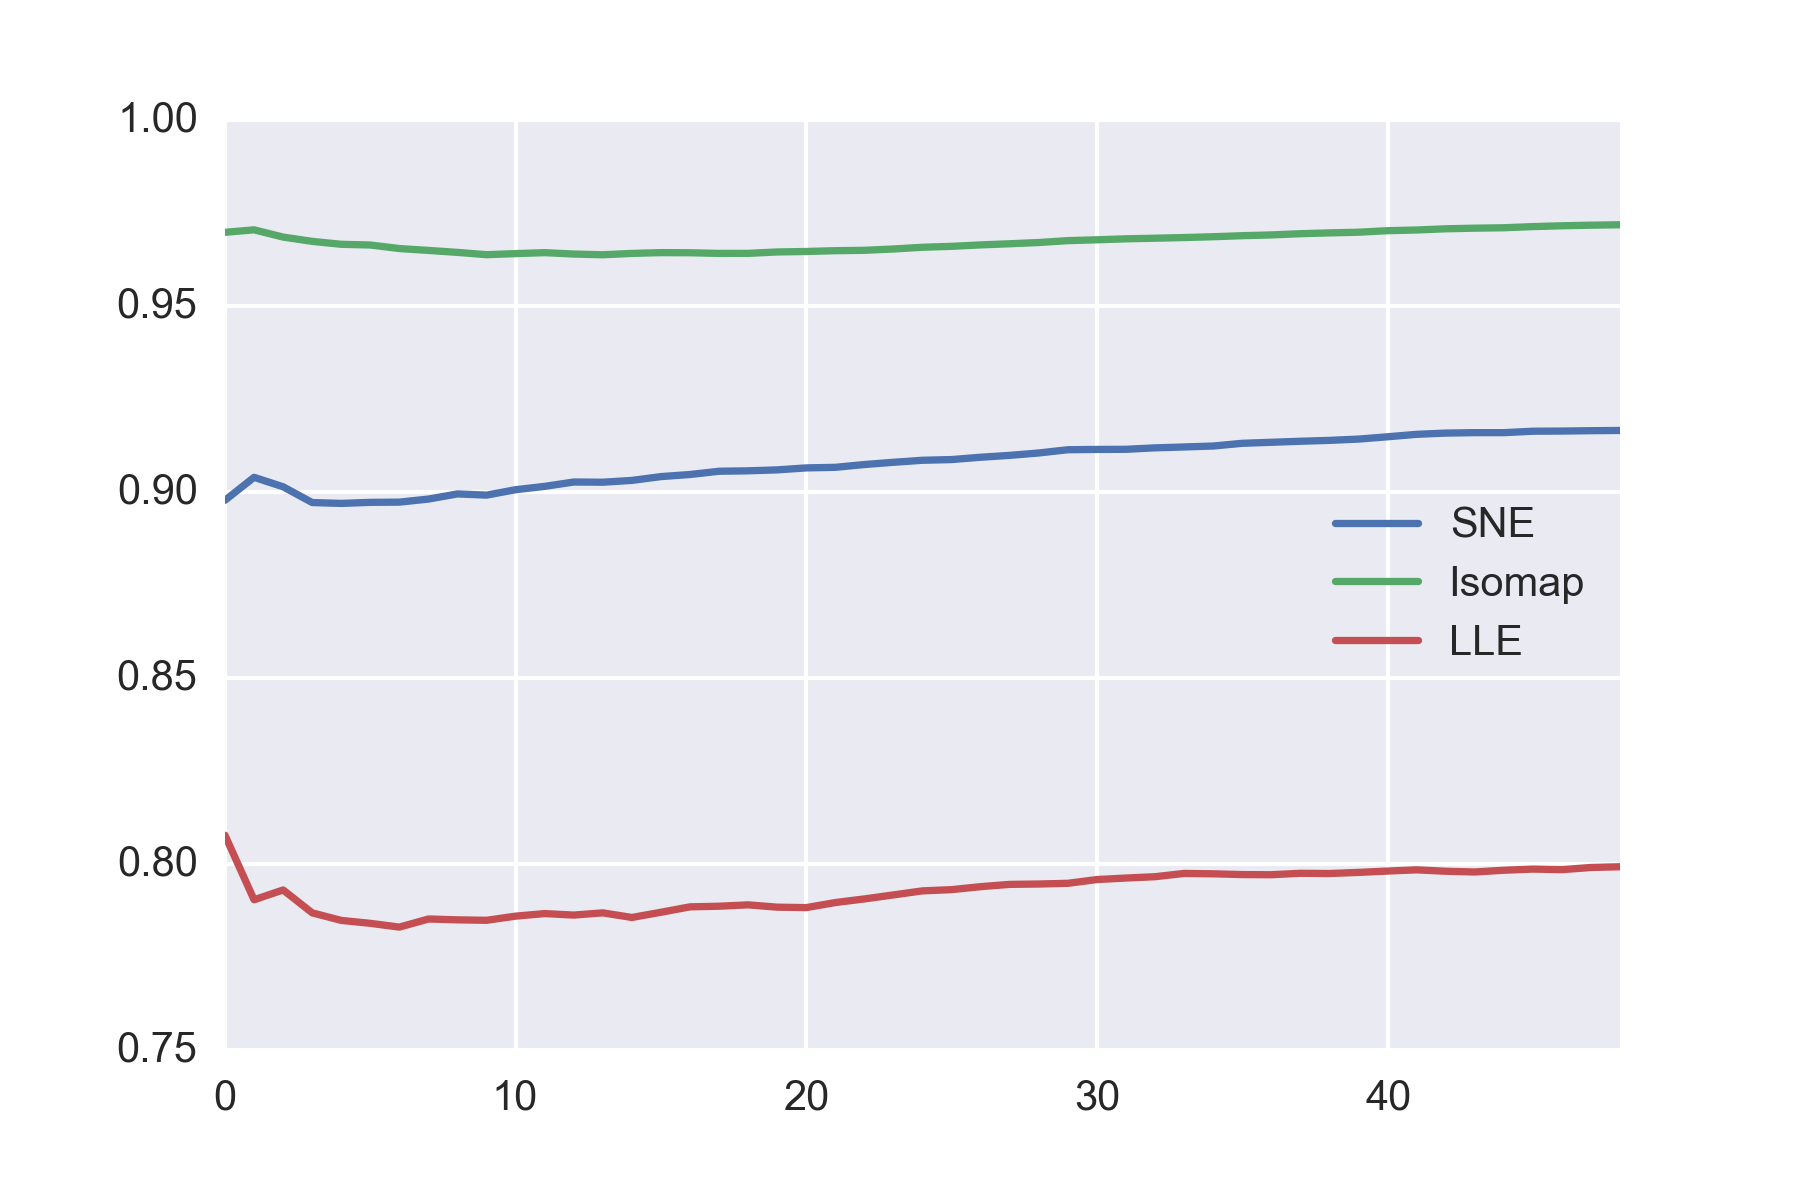
\includegraphics[width=0.49\textwidth]{figures/quality_measures/texture_continuity_3d.png}}
	\caption{Trustworthiness and continuity of the 3D projections produced from texture features from blobs.}\label{fig:TC_3d_blobs}
\end{figure}

\begin{figure}[H]
	\centering
	\subfigure{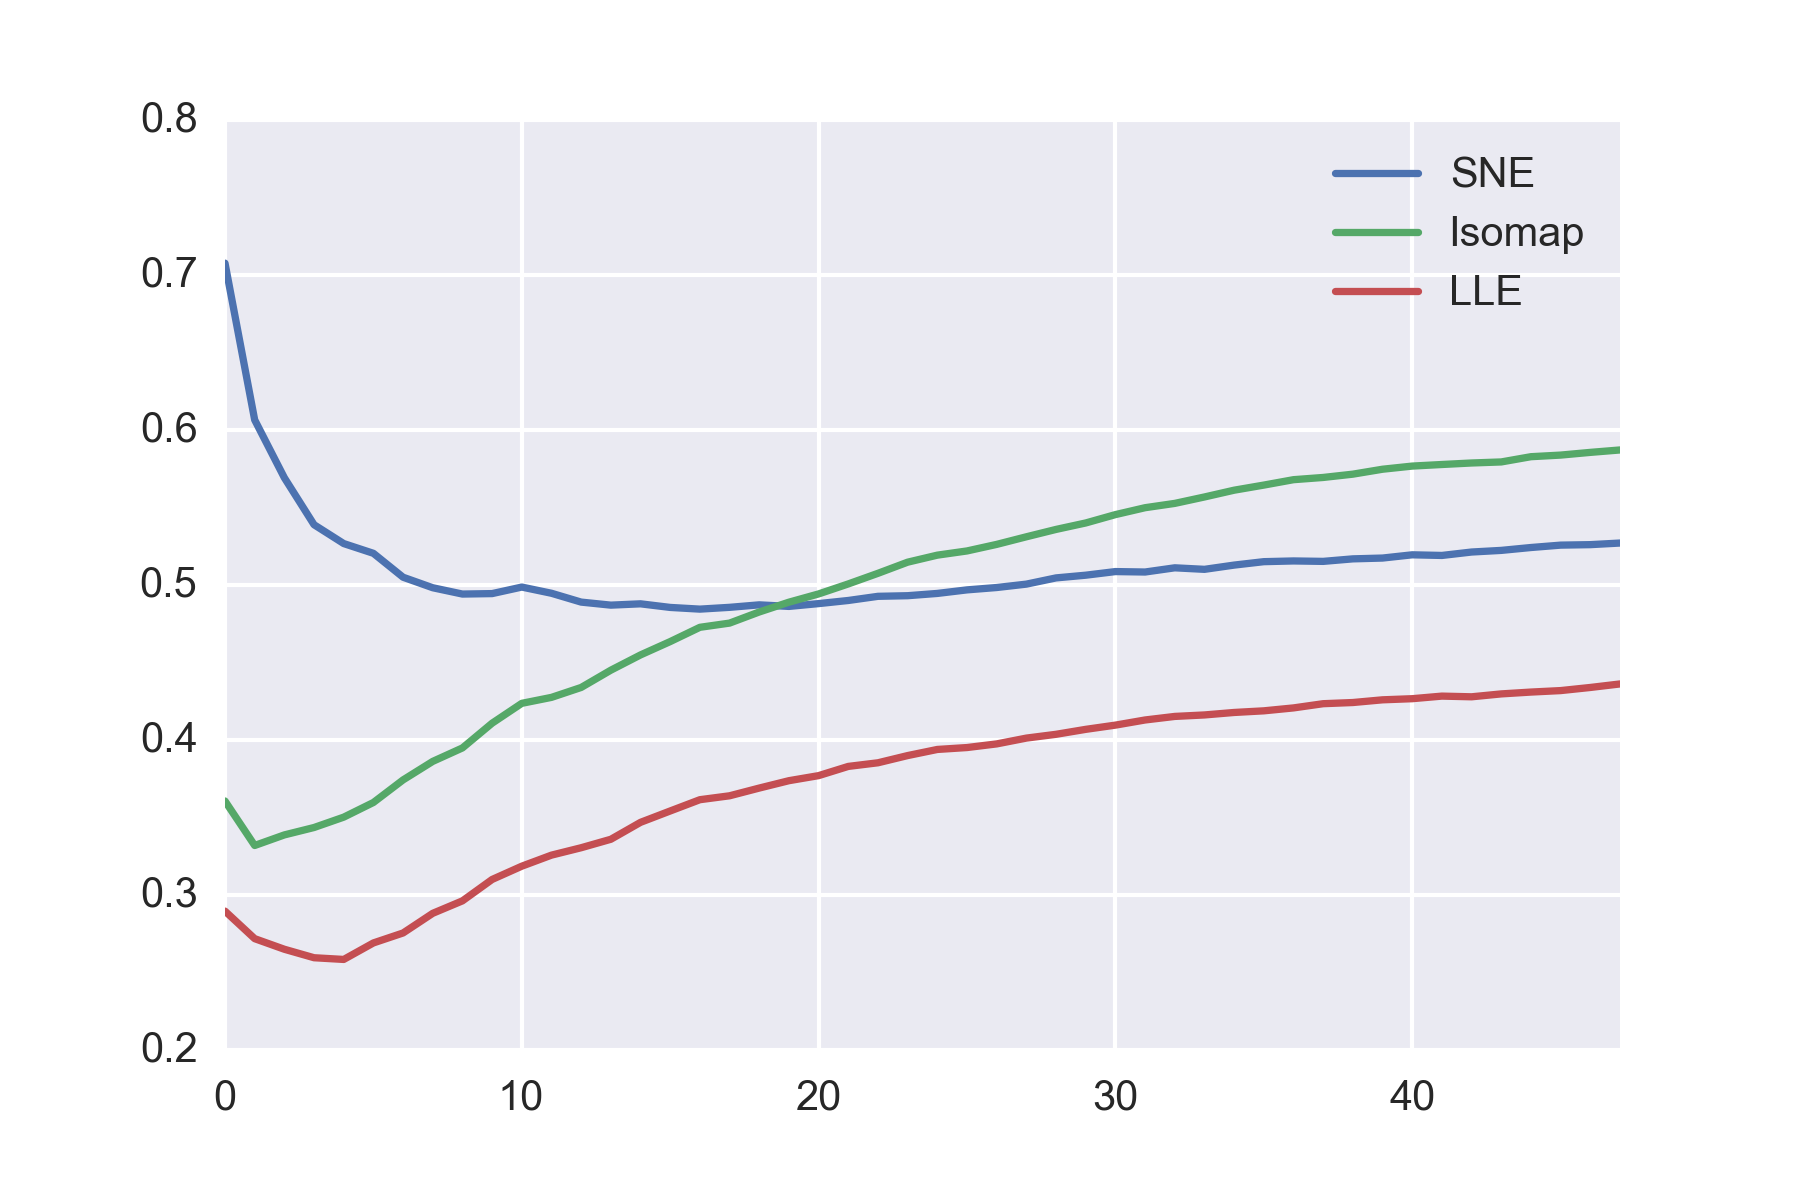
\includegraphics[width=0.49\textwidth]{figures/quality_measures/texture_lcmc_2d.png}}
	\subfigure{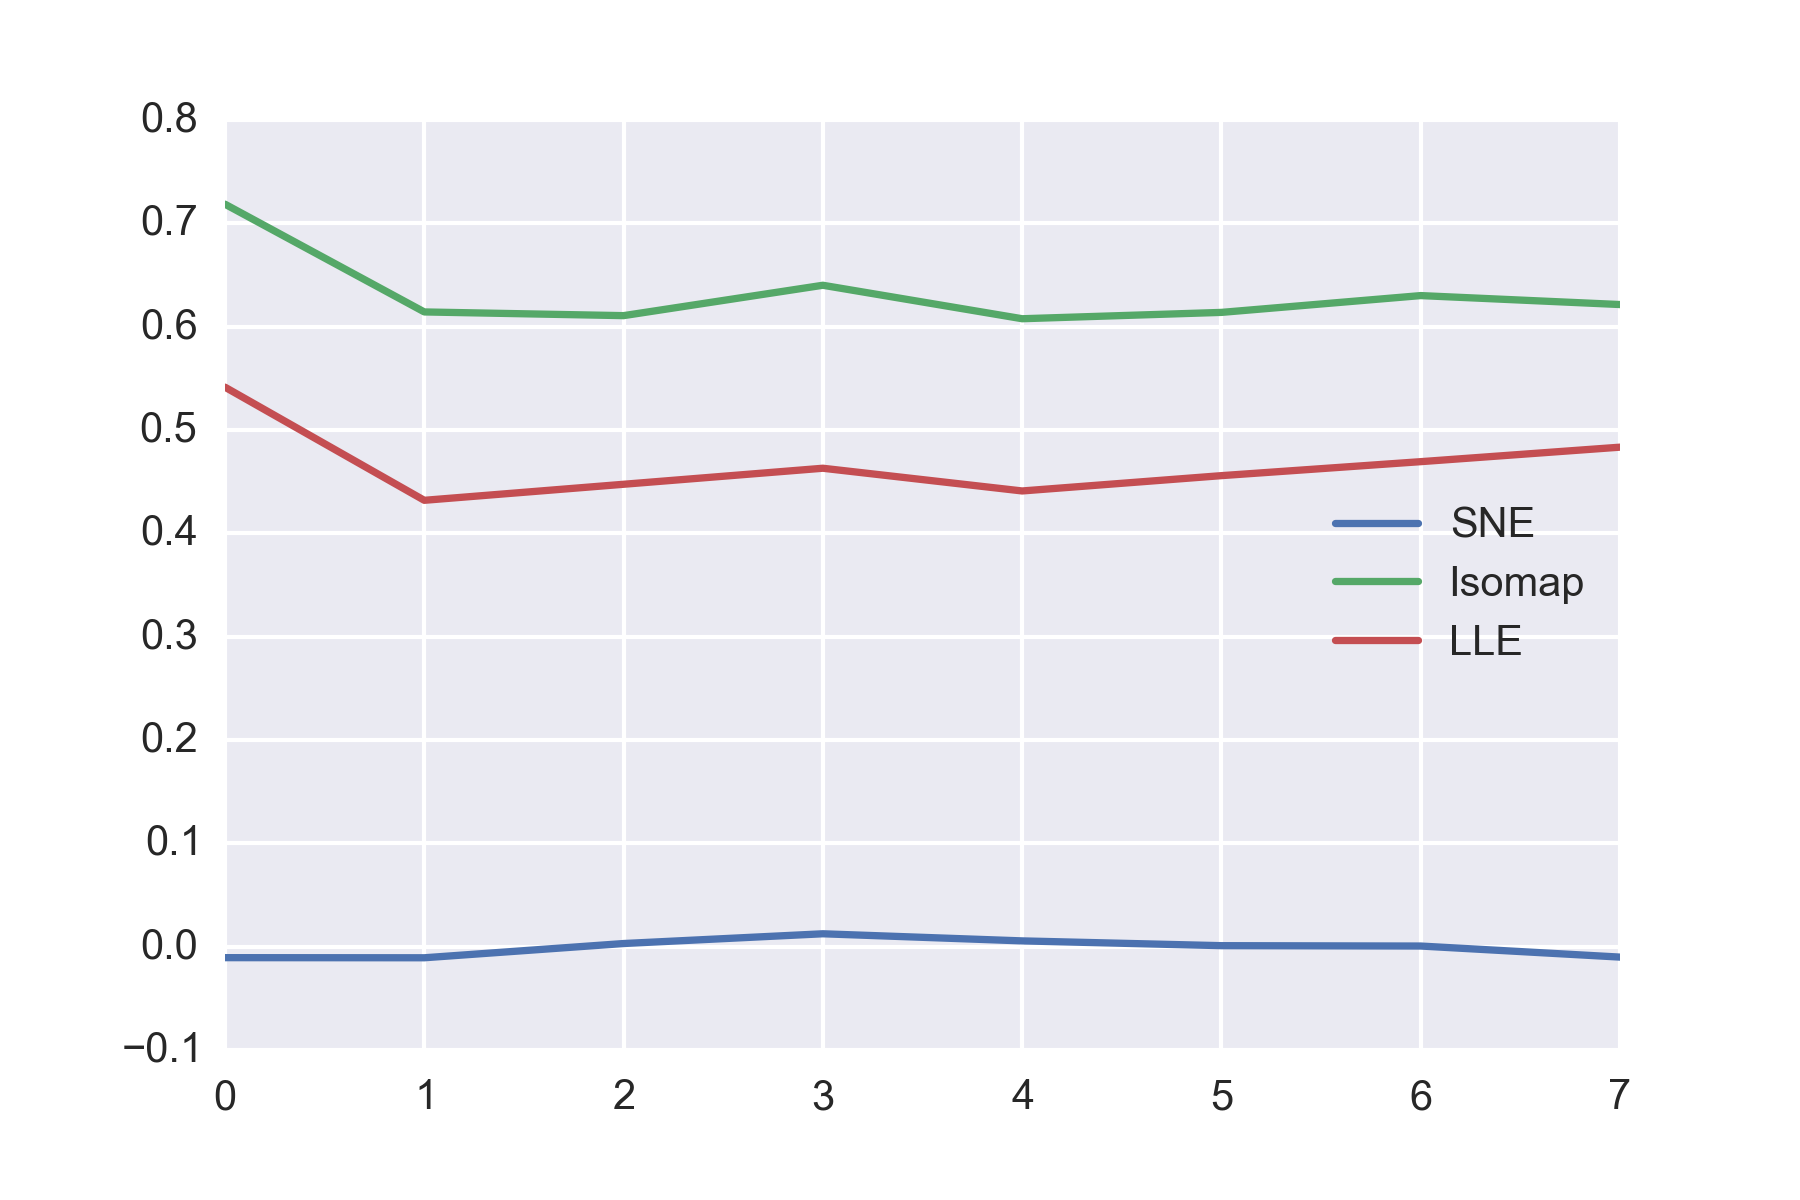
\includegraphics[width=0.49\textwidth]{figures/quality_measures/texture_lcmc_3d.png}}
	\caption{LCMC of both the 2D projection (left) and 3D projection (right) of the feature space for texture.}\label{fig:LCMC_blobs}
\end{figure}
\clearpage


